% CineLake — Báo cáo bài tập lớn Kỹ thuật dữ liệu (CO5173).
% Biên dịch bằng XeLaTeX ít nhất hai lượt để cập nhật mục lục và danh mục.
% Đặt thư mục images cùng cấp với tệp này.
\documentclass[a4paper,12pt]{article}

% ---------- Mã hóa và phông chữ ----------
\usepackage{iftex}
\ifPDFTeX
  \usepackage[utf8]{inputenc}
  \usepackage[T5]{fontenc}
\else
  \usepackage{fontspec}
\fi
\usepackage[vietnamese]{babel}
\addto\captionsvietnamese{%
  \renewcommand{\contentsname}{Mục lục}%
  \renewcommand{\listfigurename}{Danh mục hình}%
  \renewcommand{\listtablename}{Danh mục bảng}%
  \renewcommand{\figurename}{Hình}%
  \renewcommand{\tablename}{Bảng}%
}

% ---------- Bố cục trang ----------
\usepackage[a4paper,margin=2.5cm]{geometry}
\usepackage{setspace}
\onehalfspacing
\usepackage{parskip}
\setlength{\emergencystretch}{3em}
\clubpenalty=10000
\widowpenalty=10000

% ---------- Hình ảnh ----------
\usepackage{graphicx}
\usepackage{float}
\usepackage{caption}
\usepackage{needspace}
\captionsetup{font=small,labelfont=bf,labelsep=period}

% ---------- Bảng ----------
\usepackage{array}
\usepackage{tabularx}
\usepackage{booktabs}
\usepackage{longtable}
\usepackage{ragged2e}
\usepackage{textcomp}
\usepackage{enumitem}
\setlist{itemsep=0.25em,parsep=0.25em,topsep=0.35em}
\newlength{\reporttablewidth}
\setlength{\LTcapwidth}{\textwidth}

\newcolumntype{L}[1]{>{\RaggedRight\arraybackslash}p{#1}}
\newcolumntype{C}[1]{>{\centering\arraybackslash}p{#1}}

% Cho phép ngắt dòng sau dấu gạch dưới trong định danh.
\newcommand{\dbsep}{\_\allowbreak}

% ---------- Thông tin bìa ----------
\newcommand{\reporttitle}{CineLake}
\newcommand{\reportsubtitle}{%
  Lakehouse dữ liệu phim đầu cuối\\
  phục vụ phân tích và gợi ý
}
\newcommand{\coursename}{Kỹ thuật dữ liệu}
\newcommand{\coursecode}{CO5173}
\newcommand{\instructor}{PGS.\ TS.\ Võ Thị Ngọc Châu}
\newcommand{\reportsemester}{Học kỳ 1 -- Năm học 2026--2027}
\newcommand{\reportdate}{ngày 8 tháng 11 năm 2026}
\newcommand{\groupid}{24}

% ---------- Đầu trang và chân trang ----------
\usepackage{fancyhdr}
\pagestyle{fancy}
\fancyhf{}
\fancyhead[L]{\small CineLake -- Báo cáo bài tập lớn}
\fancyhead[R]{\small \coursename\ (\coursecode)}
\fancyfoot[C]{\small\thepage}
\setlength{\headheight}{16pt}
\renewcommand{\headrulewidth}{0.4pt}
\renewcommand{\footrulewidth}{0pt}

\fancypagestyle{plain}{%
  \fancyhf{}
  \fancyhead[L]{\small CineLake -- Báo cáo bài tập lớn}
  \fancyhead[R]{\small \coursename\ (\coursecode)}
  \fancyfoot[C]{\small\thepage}
  \renewcommand{\headrulewidth}{0.4pt}
  \renewcommand{\footrulewidth}{0pt}
}

% ---------- Liên kết ----------
\usepackage{xurl}
\usepackage[hidelinks,unicode]{hyperref}
\urlstyle{same}
\hypersetup{
  pdftitle={CineLake -- Báo cáo bài tập lớn Kỹ thuật dữ liệu},
  pdfauthor={Nguyễn Đình Tuấn, Lê Tuấn Hưng, Trần Anh Khoa, Nguyễn Tấn Dũng},
  pdfsubject={Lakehouse dữ liệu phim, phân tích và gợi ý},
  pdfkeywords={
    data engineering, CineLake, Databricks, Delta Lake,
    MovieLens, dimensional modeling, administration dashboard
  }
}
\setcounter{tocdepth}{2}
\setcounter{secnumdepth}{2}

\begin{document}
\hypersetup{pageanchor=false}

% =====================================================================
% Trang bìa
% =====================================================================

\begin{titlepage}
  \centering
  \setstretch{1.1}
  \setlength{\parskip}{0pt}

  {\normalsize\bfseries
    ĐẠI HỌC QUỐC GIA TP. HỒ CHÍ MINH\\
    TRƯỜNG ĐẠI HỌC BÁCH KHOA\\
    KHOA KHOA HỌC VÀ KỸ THUẬT MÁY TÍNH\par
  }

  \vspace{0.4cm}

  
\includegraphics[width=0.24\textwidth]{./images/hcmut.png}

  \par\vspace{0.4cm}

  {\LARGE\bfseries BÁO CÁO BÀI TẬP LỚN\par}
  \vspace{0.6cm}
  {\large\bfseries \coursename\ (\coursecode)\par}
  \vspace{0.3cm}
  {\normalsize \reportsemester\par}

  \vspace{1cm}
  {\Huge\bfseries \reporttitle\par}
  \vspace{0.4cm}

  \begin{minipage}{0.94\textwidth}
    \centering
    {\Large\bfseries \reportsubtitle\par}
  \end{minipage}

  \vspace{1cm}
  {\large Giảng viên hướng dẫn: \textbf{\instructor}\par}

  \ifx\groupid\empty\else
    \vspace{0.3cm}
    {\large Nhóm \groupid\par}
  \fi

  \vspace{0.7cm}
  {\large\bfseries Thành viên nhóm\par}
  \vspace{0.2cm}

  {\small
    \setstretch{1.15}
    \renewcommand{\arraystretch}{1.3}

    \begin{tabularx}{\textwidth}{
      @{}L{4.5cm}C{2.0cm}
      >{\RaggedRight\arraybackslash}X@{}
    }
      \hline
      \textbf{Họ và tên} & \textbf{MSSV} & \textbf{Email} \\
      \hline
      Nguyễn Đình Tuấn & 2670389 & \nolinkurl{tuan.nguyen0811@hcmut.edu.vn} \\
      Lê Tuấn Hưng & 2670289 & \nolinkurl{hung.lechmaster@hcmut.edu.vn} \\
      Trần Anh Khoa & 2670309 & \nolinkurl{khoa.trana@hcmut.edu.vn} \\
      Nguyễn Tấn Dũng & 2670272 & \nolinkurl{dung.nguyentan272@hcmut.edu.vn} \\
      \hline
    \end{tabularx}
  }

  \vfill
  {\large TP. Hồ Chí Minh, \reportdate\par}
\end{titlepage}

% ---------- Phần đầu báo cáo ----------
\pagenumbering{roman}
\hypersetup{pageanchor=true}
\section*{Tóm tắt}

\textbf{Lĩnh vực thực hiện.} Giải trí: nền tảng xem, chấm điểm và khám phá phim

\textbf{Hệ thống đã thực hiện của nhóm.} Web app: \url{https://cinelake.hunglechpro.id.vn} \textperiodcentered{} Databricks \textperiodcentered{} Neon PostgreSQL

CineLake là một nền tảng xem, chấm điểm và khám phá phim. Đồ án xây dựng phần kỹ thuật dữ liệu phía sau nền tảng đó: một lakehouse trên Databricks thu dữ liệu từ bốn nguồn (MovieLens 32M với 32 triệu rating thật, TMDB, IMDb và database của web app), làm sạch, kiểm soát chất lượng, rồi phục vụ 8 yêu cầu nghiệp vụ (BR) cho năm nhóm người dùng: 3 BR trên web app cho người xem và 5 BR trên dashboard cho các các bộ phận nội bộ. Thay đổi trên app được đưa vào lakehouse liên tục bằng kỹ thuật CDC (Debezium và Kafka); dữ liệu đi qua ba tầng bronze, silver, gold và 45 DQ check trước khi tới người dùng.

Kết quả đo ngày 08/11/2026 trên hệ thống đang chạy: 45/45 DQ check đạt; 789.359 rating đi qua đường CDC khớp từng dòng với dữ liệu gốc; một vòng xử lý lakehouse mất 7,6 phút; gợi ý cá nhân đạt Hit rate of 10 20,43\% so với 17,19\% của cách gợi ý phim phổ biến. Cả 8 BR đều được ứng dụng trả lời đúng trong kịch bản kiểm thử.

\clearpage
\begingroup
  \small
  \setstretch{1.0}
  \tableofcontents
  \clearpage
  \listoffigures
  \clearpage
  \listoftables
\endgroup

\clearpage
\pagenumbering{arabic}

\section{Giới thiệu}\label{sec:1}

\subsection{Bối cảnh}\label{sec:1.1}

Trong lĩnh vực giải trí, cụ thể là về phim ảnh, một nền tảng xem phim giúp người xem tìm được phim hợp gu, xem trọn vẹn thì sẽ có khả năng thu hút được người dùng. Để làm được việc đó, những nhà phát triển cần phục vụ cùng một nguồn dữ liệu ở hai nơi: thứ nhất, người xem cần gợi ý ngay trên ứng dụng; thứ hai, các đội ngũ nội bộ (internal teams) cần số liệu để vận hành và đưa ra quyết định nhằm cải thiện trải nghiệm người dùng.
\newline
Trong đề tài này, nhóm lấy cảm hứng từ cách Netflix đã giải quyết nhiều bài toán khác nhau để trở thành một trong những nền tảng xem phim trực tuyến lớn nhất lịch sử. Nhóm xây dựng CineLake để tái hiện một nền tảng xem, chấm điểm và khám phá phim từ các tập dữ liệu có sẵn, trong đó MovieLens cung cấp lịch sử chấm điểm thực tế của người dùng. Nhóm chọn mốc 28/12/2025 trên dòng thời gian của dataset MovieLens để phân tích dữ liệu. Trọng tâm của đồ án là thu thập dữ liệu từ ứng dụng và các nguồn ngoài vào Lakehouse để làm sạch, mô hình hoá và kiểm định chất lượng, phục vụ cho cả tính năng người dùng lẫn dashboard báo cáo.

\subsection{Yêu cầu nghiệp vụ}\label{sec:1.2}

Bảng~\ref{tab:01} tổng hợp các mục tiêu nghiệp vụ chính và các thước đo tương ứng mà hệ thống cần theo dõi.

\begingroup
\small
\setstretch{1.12}
\setlength{\tabcolsep}{4pt}
\renewcommand{\arraystretch}{1.18}
\setlength{\reporttablewidth}{\dimexpr\linewidth-6\tabcolsep\relax}
\begin{longtable}{@{}L{0.08\reporttablewidth} L{0.28\reporttablewidth} L{0.43\reporttablewidth} L{0.21\reporttablewidth}@{}}
\caption[Yêu cầu nghiệp vụ (mục 1.2)]{Yêu cầu nghiệp vụ}\label{tab:01} \\
\toprule
\textbf{\#} & \textbf{Mục tiêu} & \textbf{Đo bằng} & \textbf{BR phục vụ} \\
\midrule
\endfirsthead
\toprule
\textbf{\#} & \textbf{Mục tiêu} & \textbf{Đo bằng} & \textbf{BR phục vụ} \\
\midrule
\endhead
\midrule
\endfoot
\bottomrule
\endlastfoot
O1 & Tăng tương tác & Số lượt xem và chấm điểm; tỉ lệ mở trang phim dẫn tới xem & BR1, BR2, BR3, BR4, BR8 \\
O2 & Giữ chân người dùng & Tỉ lệ user quay lại tháng sau; phim đã lưu mà chưa xem & BR5, BR8 \\
O3 & Đầu tư nội dung đúng chỗ & Phim người dùng tìm mà catalog chưa có & BR7 \\
O4 & Trải nghiệm xem ổn định & Thời gian chờ phát, tỉ lệ lỗi, số phàn nàn & BR6 \\
\end{longtable}
\endgroup

\subsection{Phạm vi và đóng góp}\label{sec:1.3}

Nhóm xây dựng và vận hành một hệ thống hoàn chỉnh, dựa trên ý tưởng của ứng dụng thực tế là \textbf{Netflix}.

\begin{itemize}
  \item \textbf{Thu thập hai chiều:} kéo dữ liệu từ nguồn theo đợt, và đẩy mọi thay đổi của app vào lakehouse liên tục bằng kỹ thuật CDC.
  \item \textbf{Lakehouse có kiểm soát chất lượng:} ba tầng dữ liệu và 45 DQ check phủ 6 chiều chất lượng; dữ liệu sai bị chặn trước khi tới người dùng.
  \item \textbf{Vòng phản hồi khép kín:} kết quả của lakehouse quay về app, và hành động mới trên app lại đi vào lakehouse.
  \item \textbf{8 BR có số liệu:} 3 BR trên web app, 5 BR trên dashboard.
  \item \textbf{Kiểm thử:} 83 unit test chạy trên bảng Delta thật, cùng một code với Databricks.
\end{itemize}

Ngoài phạm vi: thanh toán và dữ liệu xem phim thật (MovieLens không có; phần này được mô phỏng, mục 2.3).

\section{Người dùng, yêu cầu nghiệp vụ và dữ liệu}\label{sec:2}

\subsection{Người dùng dữ liệu}\label{sec:2.1}

Dữ liệu của CineLake được dùng ở hai nơi: web app cho người xem, và dashboard Databricks cho các các bộ phận nội bộ.

\begingroup
\small
\setstretch{1.12}
\setlength{\tabcolsep}{4pt}
\renewcommand{\arraystretch}{1.18}
\setlength{\reporttablewidth}{\dimexpr\linewidth-6\tabcolsep\relax}
\begin{longtable}{@{}L{0.16\reporttablewidth} L{0.28\reporttablewidth} L{0.16\reporttablewidth} L{0.40\reporttablewidth}@{}}
\caption[Nhóm người dùng dữ liệu (mục 2.1)]{Nhóm người dùng dữ liệu}\label{tab:02} \\
\toprule
\textbf{Nhóm} & \textbf{Đối tượng} & \textbf{Ứng dụng} & \textbf{Thông tin cần từ dữ liệu} \\
\midrule
\endfirsthead
\toprule
\textbf{Nhóm} & \textbf{Đối tượng} & \textbf{Ứng dụng} & \textbf{Thông tin cần từ dữ liệu} \\
\midrule
\endhead
\midrule
\endfoot
\bottomrule
\endlastfoot
Viewers & Người xem & Web app & Biết nên xem gì tiếp, phim nào đang được chú ý, phim nào giống phim mình thích \\
Product & Đội sản phẩm & Dashboard & Discovery channel nào (tìm kiếm, gợi ý, trending, phim tương tự, Danh sách yêu thích) đưa người xem tới xem phim \\
Marketing và CRM & Marketing, chăm sóc khách hàng & Dashboard & Tỉ lệ giữ chân theo tháng, danh sách user cần kéo lại, phim đã lưu mà chưa xem \\
Content & Đội tìm kiếm và sản xuất nội dung & Dashboard & Phim người dùng tìm mà catalog chưa có \\
Platform & Đội phát triển phần mềm và hạ tầng & Dashboard & Thiết bị, phiên bản player nào phát kém, người dùng phàn nàn gì \\
\end{longtable}
\endgroup

Ngoài ra, đội dữ liệu dùng một dashboard vận hành riêng (CDC, pipeline, chất lượng dữ liệu) để theo dõi hệ thống; dashboard này phục vụ phần đánh giá ở mục 5, không tính là BR.

\subsection{Tám yêu cầu nghiệp vụ}\label{sec:2.2}

Phạm vi của nhóm, bao gồm 04 người, có tất cả 08 yêu cầu nghiệp vụ (Business Requirement - BR).

\begingroup
\footnotesize
\setstretch{1.12}
\setlength{\tabcolsep}{4pt}
\renewcommand{\arraystretch}{1.18}
\setlength{\reporttablewidth}{\dimexpr\linewidth-10\tabcolsep\relax}
\begin{longtable}{@{}L{0.07\reporttablewidth} L{0.14\reporttablewidth} L{0.29\reporttablewidth} L{0.09\reporttablewidth} L{0.27\reporttablewidth} L{0.14\reporttablewidth}@{}}
\caption[Tám yêu cầu nghiệp vụ và thách thức dữ liệu (mục 2.2)]{Tám yêu cầu nghiệp vụ và thách thức dữ liệu}\label{tab:03} \\
\toprule
\textbf{BR} & \textbf{Người dùng} & \textbf{Yêu cầu từ dữ liệu} & \textbf{Mục tiêu} & \textbf{Thách thức} & \textbf{Dữ liệu} \\
\midrule
\endfirsthead
\toprule
\textbf{BR} & \textbf{Người dùng} & \textbf{Yêu cầu từ dữ liệu} & \textbf{Mục tiêu} & \textbf{Thách thức} & \textbf{Dữ liệu} \\
\midrule
\endhead
\midrule
\endfoot
\bottomrule
\endlastfoot
BR1 & Viewers & Gợi ý cá nhân hóa kèm lý do, cập nhật ngay sau tương tác mới & O1 & Kết hợp lịch sử đánh giá với tương tác tức thời & Thật \\
BR2 & Viewers & Top phim thịnh hành (nhiều lượt xem/chấm nhất trong tuần) & O1 & Tổng hợp đa hành động theo cửa sổ thời gian ngắn & Thật \& Mô phỏng \\
BR3 & Viewers & Danh sách phim tương tự, bao phủ cả phim ít lượt đánh giá & O1 & Hợp nhất metadata đa nguồn để so sánh nội dung & Thật \\
BR4 & Product & Đánh giá kênh khám phá (discovery channel) dẫn tới lượt xem & O1 & Ghép chuỗi sự kiện từ mở trang đến xem phim & Mô phỏng \\
BR5 & Marketing & Tỷ lệ giữ chân người dùng (retention) theo từng tháng & O2 & Xây dựng lịch sử hoạt động tháng từ đa nguồn tương tác & Thật \& Mô phỏng \\
BR6 & Platform & Giám sát chất lượng phát (QoS) theo thiết bị và phiên bản app & O4 & Ghép sự kiện phát video với phản hồi/khiếu nại & Mô phỏng \\
BR7 & Content & Danh sách phim được tìm kiếm nhiều nhưng catalog chưa có & O3 & Đối chiếu từ khóa tìm kiếm với danh mục catalog & Mô phỏng \\
BR8 & Marketing & Hiệu quả Danh sách yêu thích và tỷ lệ xem phim đã lưu & O1, O2 & Truy vết lịch sử lưu/bỏ lưu qua log CDC & Mô phỏng \\
\end{longtable}
\endgroup

\subsection{Nguồn dữ liệu}\label{sec:2.3}

Bao gồm bốn nguồn, trong đó nguồn nào cũng được áp dụng cho ít nhất một BR:

\begingroup
\small
\setstretch{1.12}
\setlength{\tabcolsep}{4pt}
\renewcommand{\arraystretch}{1.18}
\setlength{\reporttablewidth}{\dimexpr\linewidth-6\tabcolsep\relax}
\begin{longtable}{@{}L{0.23\reporttablewidth} L{0.31\reporttablewidth} L{0.21\reporttablewidth} L{0.25\reporttablewidth}@{}}
\caption[Bốn nguồn dữ liệu (mục 2.3)]{Bốn nguồn dữ liệu}\label{tab:04} \\
\toprule
\textbf{Nguồn} & \textbf{Nội dung} & \textbf{Cách thu} & \textbf{Áp dụng} \\
\midrule
\endfirsthead
\toprule
\textbf{Nguồn} & \textbf{Nội dung} & \textbf{Cách thu} & \textbf{Áp dụng} \\
\midrule
\endhead
\midrule
\endfoot
\bottomrule
\endlastfoot
MovieLens 32M (GroupLens) & 32 triệu rating và 2 triệu tag thật của 200.948 người & Tải file, một lần & BR1, BR2, BR3, BR5 \\
TMDB API & Thông tin phim: tên, năm, thể loại, từ khoá, poster & Gọi API, chỉ lấy phần thay đổi & Catalog cho mọi BR và web app; BR3 \\
IMDb datasets & Điểm IMDb, đạo diễn, diễn viên, tên tiếng Việt & Tải file TSV & Trang phim; BR3 \\
Database của web app (Neon PostgreSQL) & User, rating, tag, tìm kiếm, Danh sách yêu thích, sự kiện xem và phản hồi & CDC, liên tục & Cả 8 BR \\
\end{longtable}
\endgroup

Ba nguồn ngoài được nối với nhau bằng bảng liên kết có sẵn của MovieLens, ánh xạ mỗi phim sang mã TMDB và mã IMDb.

\textbf{Dòng thời gian.} Rating MovieLens vốn trải từ 1995 đến 2023. Nhóm dời toàn bộ sang dòng thời gian 1998 \ensuremath{\rightarrow} 09/10/2026, giữ nguyên thứ tự và khoảng cách giữa các rating. Phần trước ngày ra mắt 28/12/2025 là lịch sử, được nạp theo đợt. Phần từ ngày ra mắt được phát lại qua web app, nên đi vào lakehouse qua đúng đường CDC như một hoạt động thật.

\textbf{Dữ liệu thật và dữ liệu mô phỏng.} MovieLens chỉ có rating và tag; lượt xem, tìm kiếm, lưu phim và phản hồi phải mô phỏng. Nhóm viết một simulator sinh các hành động này qua đúng các hàm của app, theo gu và nhịp hoạt động của chính từng user.

Dữ liệu mô phỏng luôn nhận ra được qua loại tài khoản:

\begin{itemize}
  \item user MovieLens: rating và tag là dữ liệu thật được phát lại, mọi hoạt động khác là mô phỏng;
  \item user do simulator tạo: toàn bộ là mô phỏng;
  \item 10 tài khoản app: người dùng thật (thành viên nhóm và tài khoản kiểm thử).
\end{itemize}

Bảng dưới đếm hoạt động theo loại tài khoản ở tầng gold ngày 08/11/2026:

\begingroup
\small
\setstretch{1.12}
\setlength{\tabcolsep}{4pt}
\renewcommand{\arraystretch}{1.18}
\setlength{\reporttablewidth}{\dimexpr\linewidth-6\tabcolsep\relax}
\begin{longtable}{@{}L{0.26\reporttablewidth} L{0.23\reporttablewidth} L{0.24\reporttablewidth} L{0.27\reporttablewidth}@{}}
\caption[Hoạt động theo loại tài khoản (mục 2.3)]{Hoạt động theo loại tài khoản (tầng gold, 08/11/2026)}\label{tab:05} \\
\toprule
\textbf{Hoạt động} & \textbf{User MovieLens} & \textbf{User do simulator tạo} & \textbf{Tài khoản thật trên app} \\
\midrule
\endfirsthead
\toprule
\textbf{Hoạt động} & \textbf{User MovieLens} & \textbf{User do simulator tạo} & \textbf{Tài khoản thật trên app} \\
\midrule
\endhead
\midrule
\endfoot
\bottomrule
\endlastfoot
Số tài khoản & 200.948 & 1.467 & 10 \\
Lượt mở trang phim & 1.098.324 & 47.273 & 29 \\
Lượt xem phim & 32.650 & 15.798 & 12 \\
Lượt tìm kiếm & 35.636 & 15.646 & 7 \\
Lần lưu phim & 22.318 & 3.789 & 7 \\
Phản hồi & 1.213 & 632 & 2 \\
Rating ghi qua app (ngoài phần phát lại) & 71.825 & 21.702 & 8 \\
\end{longtable}
\endgroup

Pipeline xử lý dữ liệu mô phỏng y hệt dữ liệu thật (cùng đường CDC, cùng DQ check), nên các chỉ số tổng trên dashboard là số của toàn bộ bộ dữ liệu dự án. Vì vậy kết quả BR cần đọc theo cột Dữ liệu của Bảng 3: BR1 và BR3 đo trên rating thật; BR2 và BR5 cần đọc thận trọng phần sau 09/10/2026; BR4, BR6, BR7, BR8 chứng minh pipeline đo được, chưa phải kết luận kinh doanh.

\subsection{Đặc tính dữ liệu và thách thức}\label{sec:2.4}

\begingroup
\small
\setstretch{1.12}
\setlength{\tabcolsep}{4pt}
\renewcommand{\arraystretch}{1.18}
\setlength{\reporttablewidth}{\dimexpr\linewidth-4\tabcolsep\relax}
\begin{longtable}{@{}L{0.15\reporttablewidth} L{0.40\reporttablewidth} L{0.45\reporttablewidth}@{}}
\caption[Đặc tính dữ liệu và thách thức (mục 2.4)]{Đặc tính dữ liệu và thách thức}\label{tab:06} \\
\toprule
\textbf{Đặc tính} & \textbf{Biểu hiện trong CineLake} & \textbf{Thách thức} \\
\midrule
\endfirsthead
\toprule
\textbf{Đặc tính} & \textbf{Biểu hiện trong CineLake} & \textbf{Thách thức} \\
\midrule
\endhead
\midrule
\endfoot
\bottomrule
\endlastfoot
Volume & 233 triệu dòng ở tầng bronze, trong đó IMDb 193 triệu & Không thể xử lý trên một máy; phải lọc sớm và xử lý phân tán \\
Velocity & Mọi thay đổi trên app phải vào lakehouse; tới 08/11/2026 đã có 5,6 triệu thay đổi đi qua CDC & Không được mất, không được trùng khi một bước lỗi rồi chạy lại \\
Variety & File CSV, file TSV, JSON từ API, sự kiện CDC & Mỗi nguồn một định dạng và một loại mã phim, phải thống nhất \\
Veracity & Nguồn có lỗi thật (dưới đây) & Phải phát hiện và chặn lỗi trước khi tới người dùng \\
\end{longtable}
\endgroup

\begin{quote}
\textbf{Lỗi thật trong dữ liệu nguồn.} 1.194 phim có mã TMDB nhưng TMDB không còn trả về, 122 phim không có liên kết nào; 177 phim có năm phát hành lệch giữa MovieLens và TMDB. Pipeline giữ các phim này nhưng gắn flag cảnh báo, thay vì âm thầm bỏ đi hoặc để lọt tới app.
\end{quote}

\section{Giải pháp kỹ thuật dữ liệu}\label{sec:3}

\subsection{Công nghệ sử dụng}\label{sec:3.1}

Khi chọn công nghệ, nhóm đặt ra ba điều kiện: chạy được miễn phí, đủ sức xử lý vài trăm triệu dòng, và gần với cách các hệ thống dữ liệu thực tế đang làm. Phần này giới thiệu nền tảng lakehouse trước (Databricks, Delta Lake, Unity Catalog), rồi tới các công nghệ thu thập, xử lý, kiểm soát chất lượng, điều phối và hiển thị dữ liệu; mỗi công nghệ kèm lý do nhóm chọn và cách nó được dùng trong CineLake. Mục 3.2 ghép các công nghệ này thành kiến trúc tổng thể của hệ thống.

\Needspace{9\baselineskip}
\subsubsection*{Databricks và mô hình lakehouse}

\noindent

\includegraphics[height=2.45cm,width=\linewidth,keepaspectratio]{./images/cong-nghe-databricks.png}\par

Trước khi có lakehouse, các tổ chức thường giữ hai hệ thống song song: một data lake trên object storage để chứa mọi loại file với chi phí thấp, và một data warehouse để chạy SQL nhanh cho báo cáo. Dữ liệu phải chép qua lại giữa hai nơi, dễ lệch nhau và tốn công vận hành. Lakehouse, được Armbrust và cộng sự mô tả năm 2021, đặt một lớp quản lý giao dịch và metadata ngay trên data lake, để cùng một bản dữ liệu phục vụ được cả xử lý khối lượng lớn lẫn truy vấn SQL. Databricks là nền tảng đi đầu theo hướng này, do chính nhóm tác giả Apache Spark sáng lập.

CineLake vừa có file thô (CSV của MovieLens, TSV của IMDb, JSON từ TMDB và từ CDC) vừa cần bảng phân tích cho dashboard, nên lakehouse là kiến trúc phù hợp. Nhóm dùng bản Databricks Free Edition: miễn phí, chỉ có compute serverless nên không phải tự cấu hình cluster, và có sẵn các thành phần được giới thiệu bên dưới. Toàn bộ ba tầng dữ liệu, 7 job và 2 dashboard của nhóm chạy trên một workspace.

\Needspace{9\baselineskip}
\subsubsection*{Delta Lake}

\noindent

\includegraphics[height=2.45cm,width=\linewidth,keepaspectratio]{./images/cong-nghe-delta-lake.png}\par

Delta Lake là định dạng bảng mã nguồn mở, chính là lớp biến data lake thành lakehouse. Dữ liệu vẫn nằm trong các file Parquet, nhưng mỗi lần ghi được ghi thêm vào một transaction log. Nhờ transaction log này, người đọc không bao giờ thấy dữ liệu ghi dở (giao dịch ACID), bảng hỗ trợ UPDATE, DELETE và MERGE như một database, và mỗi lần ghi tạo ra một phiên bản mới có thể đọc lại về sau (time travel).

Trong CineLake, mọi bảng bronze, silver và gold đều là bảng Delta. MERGE là tính năng quan trọng nhất, vì thay đổi từ app gồm cả sửa và xoá chứ không chỉ thêm; mục 3.4 cho thấy MERGE theo thứ tự LSN giúp chạy lại bao nhiêu lần cũng không sinh sai. Time travel cũng được dùng thật: bước serving so số phiên bản để bỏ qua bảng không đổi, và một số số liệu ngày 08/11 trong báo cáo được đọc lại đúng phiên bản bảng lúc vòng daily kết thúc.

\Needspace{9\baselineskip}
\subsubsection*{Unity Catalog}

\noindent

\includegraphics[height=2.45cm,width=\linewidth,keepaspectratio]{./images/cong-nghe-unity-catalog.png}\par

Unity Catalog là lớp quản trị dữ liệu của Databricks. Mọi tài sản dữ liệu được tổ chức theo ba cấp catalog, schema, bảng; quyền truy cập được cấp ở bất kỳ cấp nào bằng câu lệnh GRANT. Ngoài bảng, Unity Catalog còn quản lý Volume (vùng chứa file không phải bảng) và lưu vết ai đã đọc, ghi dữ liệu nào.

Nhóm dùng mỗi schema cho một vai trò: bronze, silver, gold cho ba tầng, dq cho kết quả kiểm tra chất lượng, ops cho nhật ký vận hành. File thô từ nguồn và từ CDC nằm trong một Volume riêng. Token TMDB và thông tin kết nối PostgreSQL được lưu trong secret, nên không xuất hiện trong code hay trong Git. Đây là cách nhóm đáp ứng yêu cầu về quản trị và bảo mật của đề mà không phải tự dựng hệ thống phân quyền.

\Needspace{9\baselineskip}
\subsubsection*{PostgreSQL trên Neon}

\noindent

\includegraphics[height=2.45cm,width=\linewidth,keepaspectratio]{./images/cong-nghe-postgresql-neon.png}\par

PostgreSQL là database quan hệ mã nguồn mở, mạnh ở xử lý giao dịch (OLTP): rất nhiều thao tác nhỏ, diễn ra cùng lúc, cần trả lời trong mili giây. Neon cung cấp PostgreSQL dạng serverless, tách lưu trữ khỏi tính toán và tự tắt khi không dùng, có gói miễn phí và hỗ trợ logical replication.

Web app cần đúng loại database này, việc mà lakehouse không làm tốt. Database trên Neon có hai schema chính (mục 3.3 mô tả đủ bốn schema): schema app chứa dữ liệu vận hành, chỉ ghi được qua các hàm SQL định nghĩa sẵn để mọi thao tác theo cùng một quy tắc; schema serving chứa kết quả do lakehouse trả về. Gợi ý online cũng được tính ngay tại đây bằng một hàm SQL (mục 3.6). Logical replication là điều kiện để Debezium đọc được các thay đổi.

\Needspace{9\baselineskip}
\subsubsection*{Debezium và kỹ thuật CDC}

\noindent

\includegraphics[height=2.45cm,width=\linewidth,keepaspectratio]{./images/cong-nghe-debezium.png}\par

Change Data Capture (CDC) là kỹ thuật ghi lại từng thay đổi của database để hệ thống khác dùng. Có hai cách phổ biến: định kỳ hỏi các dòng có thời điểm cập nhật mới (query-based), hoặc đọc transaction log của chính database (log-based). Cách thứ hai không thêm tải truy vấn, thấy được cả lệnh xoá và giữ đúng thứ tự commit. Debezium là công cụ CDC log-based mã nguồn mở phổ biến nhất, chạy như một connector trên Kafka Connect. Với PostgreSQL, Debezium đọc Write-Ahead Log (WAL) qua một replication slot, và mỗi thay đổi mang một số thứ tự LSN chỉ tăng.

Nhóm chọn cách log-based vì BR8 cần biết lúc người dùng bỏ phim khỏi Danh sách yêu thích, mà dòng đó bị xoá hẳn trong database của app; cách hỏi định kỳ sẽ không bao giờ thấy nó. Debezium theo dõi 6 bảng của app, mỗi bảng ra một topic Kafka, và số LSN đi kèm được lakehouse dùng để biết thay đổi nào mới hơn.

\Needspace{9\baselineskip}
\subsubsection*{Apache Kafka}

\noindent
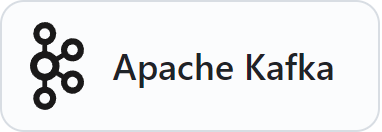
\includegraphics[height=2.45cm,width=\linewidth,keepaspectratio]{./images/cong-nghe-apache-kafka.png}\par

Kafka là nền tảng truyền sự kiện phân tán. Sự kiện được ghi vào topic như một nhật ký chỉ thêm, chia thành nhiều partition để xử lý song song. Bên đọc tự giữ vị trí đã đọc (offset), nên nhiều bên đọc hoạt động độc lập với tốc độ riêng, và dữ liệu được giữ theo thời gian cấu hình chứ không mất đi khi đã được đọc.

Trong CineLake, Kafka là buffer giữa database và lakehouse: sự kiện được giữ 7 ngày, nên khi phía Databricks tạm dừng thì không mất gì. Compute serverless của Free Edition không kết nối được tới Kafka trên server riêng, nên nhóm viết một chương trình sink đọc Kafka, gom sự kiện thành file rồi đẩy lên Volume (chi tiết ở mục 3.3). Debezium, Kafka và sink chạy bằng Docker Compose trên một server riêng, liên tục 24/7.

\Needspace{9\baselineskip}
\subsubsection*{Apache Spark, Structured Streaming và Auto Loader}

\noindent

\includegraphics[height=2.45cm,width=\linewidth,keepaspectratio]{./images/cong-nghe-apache-spark.png}\par

Spark là engine xử lý dữ liệu phân tán: một job được chia thành nhiều tác vụ chạy song song trên nhiều máy, với API DataFrame và SQL quen thuộc. Structured Streaming là phần xử lý luồng của Spark, coi dữ liệu mới như các dòng nối thêm vào một bảng không có điểm cuối, xử lý theo từng đợt nhỏ (micro-batch) và ghi tiến độ vào checkpoint để không xử lý lặp. Auto Loader là nguồn đọc của Databricks dành cho Structured Streaming, tự phát hiện file mới trong một thư mục mà không phải liệt kê lại toàn bộ.

32 triệu rating và 193 triệu dòng IMDb vượt quá khả năng xử lý trên một máy, nên Spark gần như là lựa chọn bắt buộc. Nhóm dùng Auto Loader và Structured Streaming để nạp file vào bronze và đưa phần mới sang silver, ở chế độ trigger availableNow, đọc hết phần mới rồi dừng thay vì chạy liên tục, vừa đủ tươi vừa hợp hạn mức của Free Edition.

Các bước nặng như dựng gold và tính độ giống giữa 83 nghìn phim dùng Spark batch. Logic biến đổi được viết thành hàm DataFrame thuần, nên chạy được cả trên Databricks lẫn trong 83 unit test trên máy cá nhân.

\Needspace{9\baselineskip}
\subsubsection*{Databricks DQX}

\noindent

\includegraphics[height=2.45cm,width=\linewidth,keepaspectratio]{./images/cong-nghe-databricks-dqx.png}\par

DQX là thư viện kiểm tra chất lượng dữ liệu của Databricks Labs, chạy trên Spark DataFrame; mã nguồn công khai nhưng giấy phép chỉ cho dùng cùng nền tảng Databricks. Mỗi rule khai báo một điều kiện, một mức độ (error hoặc warn) và cách xử lý dòng vi phạm: tách sang bảng quarantine, gắn flag ngay trên dòng, hoặc chỉ ghi nhận. Kết quả mỗi lần kiểm tra được ghi thành bảng để theo dõi theo thời gian.

Nhóm chọn DQX vì rule được viết trong file YAML, nằm trong Git và được review như code, thay vì rải rác trong các notebook. CineLake có 45 DQ check sau từng tầng và 20 quarantine rule chạy trên từng thay đổi CDC; một rule mức error không đạt thì pipeline dừng trước khi dữ liệu tới người dùng (mục 3.5).

\Needspace{9\baselineskip}
\subsubsection*{Databricks Jobs và Asset Bundles}

\noindent

\includegraphics[height=2.45cm,width=\linewidth,keepaspectratio]{./images/cong-nghe-databricks-jobs-asset-bundles.png}\par

Databricks Jobs là bộ điều phối có sẵn của nền tảng: một job gồm nhiều task có quan hệ phụ thuộc, chạy theo lịch, theo yêu cầu hoặc khi có file mới xuất hiện (file arrival trigger), có sẵn cơ chế chạy lại và báo lỗi. Asset Bundles cho phép khai báo job, code và dashboard bằng file cấu hình YAML rồi triển khai lên workspace bằng một lệnh, theo tinh thần infrastructure as code.

Nhờ có sẵn bộ điều phối, nhóm không phải dựng thêm Airflow. Cách chia job theo tầng và cách các job được kích hoạt được trình bày ở mục 3.7. Vì mọi thứ nằm trong Git, cả nhóm dùng chung một cấu hình và dựng lại được toàn bộ trên một workspace mới.

\Needspace{9\baselineskip}
\subsubsection*{Databricks AI/BI Dashboard}

\noindent

\includegraphics[height=2.45cm,width=\linewidth,keepaspectratio]{./images/cong-nghe-databricks-aibi.png}\par

AI/BI Dashboard là công cụ BI tích hợp trong Databricks: mỗi widget là một truy vấn SQL chạy trên SQL warehouse, hiển thị thành biểu đồ, bảng hay ô chỉ số, kèm bộ lọc cho người xem. Dashboard có thể được định nghĩa bằng file và triển khai cùng Asset Bundles.

Vì dashboard đọc thẳng bảng gold, nhóm không phải chép dữ liệu sang công cụ BI khác, và quyền xem đi theo Unity Catalog. CineLake có hai dashboard: dashboard phân tích đáp ứng BR4--BR8 cho các các bộ phận nội bộ, và dashboard vận hành theo dõi CDC, pipeline và chất lượng dữ liệu cho đội dữ liệu.

\subsubsection*{Cách khai thác dữ liệu cho ứng dụng}

\begingroup
\small
\setstretch{1.12}
\setlength{\tabcolsep}{4pt}
\renewcommand{\arraystretch}{1.18}
\setlength{\reporttablewidth}{\dimexpr\linewidth-4\tabcolsep\relax}
\begin{longtable}{@{}L{0.32\reporttablewidth} L{0.24\reporttablewidth} L{0.44\reporttablewidth}@{}}
\caption[Mục đích các công nghệ được sử dụng (mục 3.1)]{Phân vai công nghệ khi khai thác dữ liệu}\label{tab:07} \\
\toprule
\textbf{Yêu cầu} & \textbf{Công nghệ} & \textbf{Lý do} \\
\midrule
\endfirsthead
\toprule
\textbf{Yêu cầu} & \textbf{Công nghệ} & \textbf{Lý do} \\
\midrule
\endhead
\midrule
\endfoot
\bottomrule
\endlastfoot
Trả lời web app trong mili giây & PostgreSQL & Database transaction, hot data\\
Record linkage, làm sạch dữ liệu, giữ toàn bộ lịch sử & Lakehouse (Spark, Delta) & Khối lượng lớn, cần xử lý phân tán \\
Phản ứng với hành động vừa xảy ra & Hàm SQL trong PostgreSQL & Không phải chờ một vòng lakehouse \\
Phân tích cho các bộ phận nội bộ & Dashboard đọc tầng gold & Bảng đã tổng hợp sẵn \\
\end{longtable}
\endgroup

\textbf{Giới hạn của Databricks Free Edition} ảnh hưởng tới thiết kế ở ba chỗ. Chỉ có compute serverless và hạn mức tính toán theo ngày, nên lakehouse xử lý theo từng vòng thay vì chạy liên tục, còn phản hồi real-time giao cho PostgreSQL. Compute không kết nối được tới Kafka trên server riêng, nên server chủ động đẩy file lên Volume. Chỉ có một SQL warehouse nhỏ, nên dashboard đọc bảng đã tổng hợp thay vì bảng 32 triệu dòng.

\subsection{Kiến trúc tổng thể}\label{sec:3.2}

Các công nghệ ở mục 3.1 được ghép thành một vòng dữ liệu khép kín. Người dùng thao tác trên web app, thao tác được ghi vào database PostgreSQL; CDC đưa từng thay đổi vào lakehouse trên Databricks; lakehouse tính kết quả rồi chép ngược về PostgreSQL cho web app đọc, và đưa lên dashboard cho các các bộ phận nội bộ. Dữ liệu đi theo ba hướng:

\begin{itemize}
  \item \textbf{Kéo (pull):} Databricks tải MovieLens, IMDb và gọi API TMDB theo đợt.
  \item \textbf{Đẩy (push):} một server riêng đọc nhật ký thay đổi của PostgreSQL và đẩy liên tục vào Databricks.
  \item \textbf{Trả về (reverse ETL):} kết quả ở tầng gold được chép về PostgreSQL.
\end{itemize}

\begin{figure}[H]
\centering
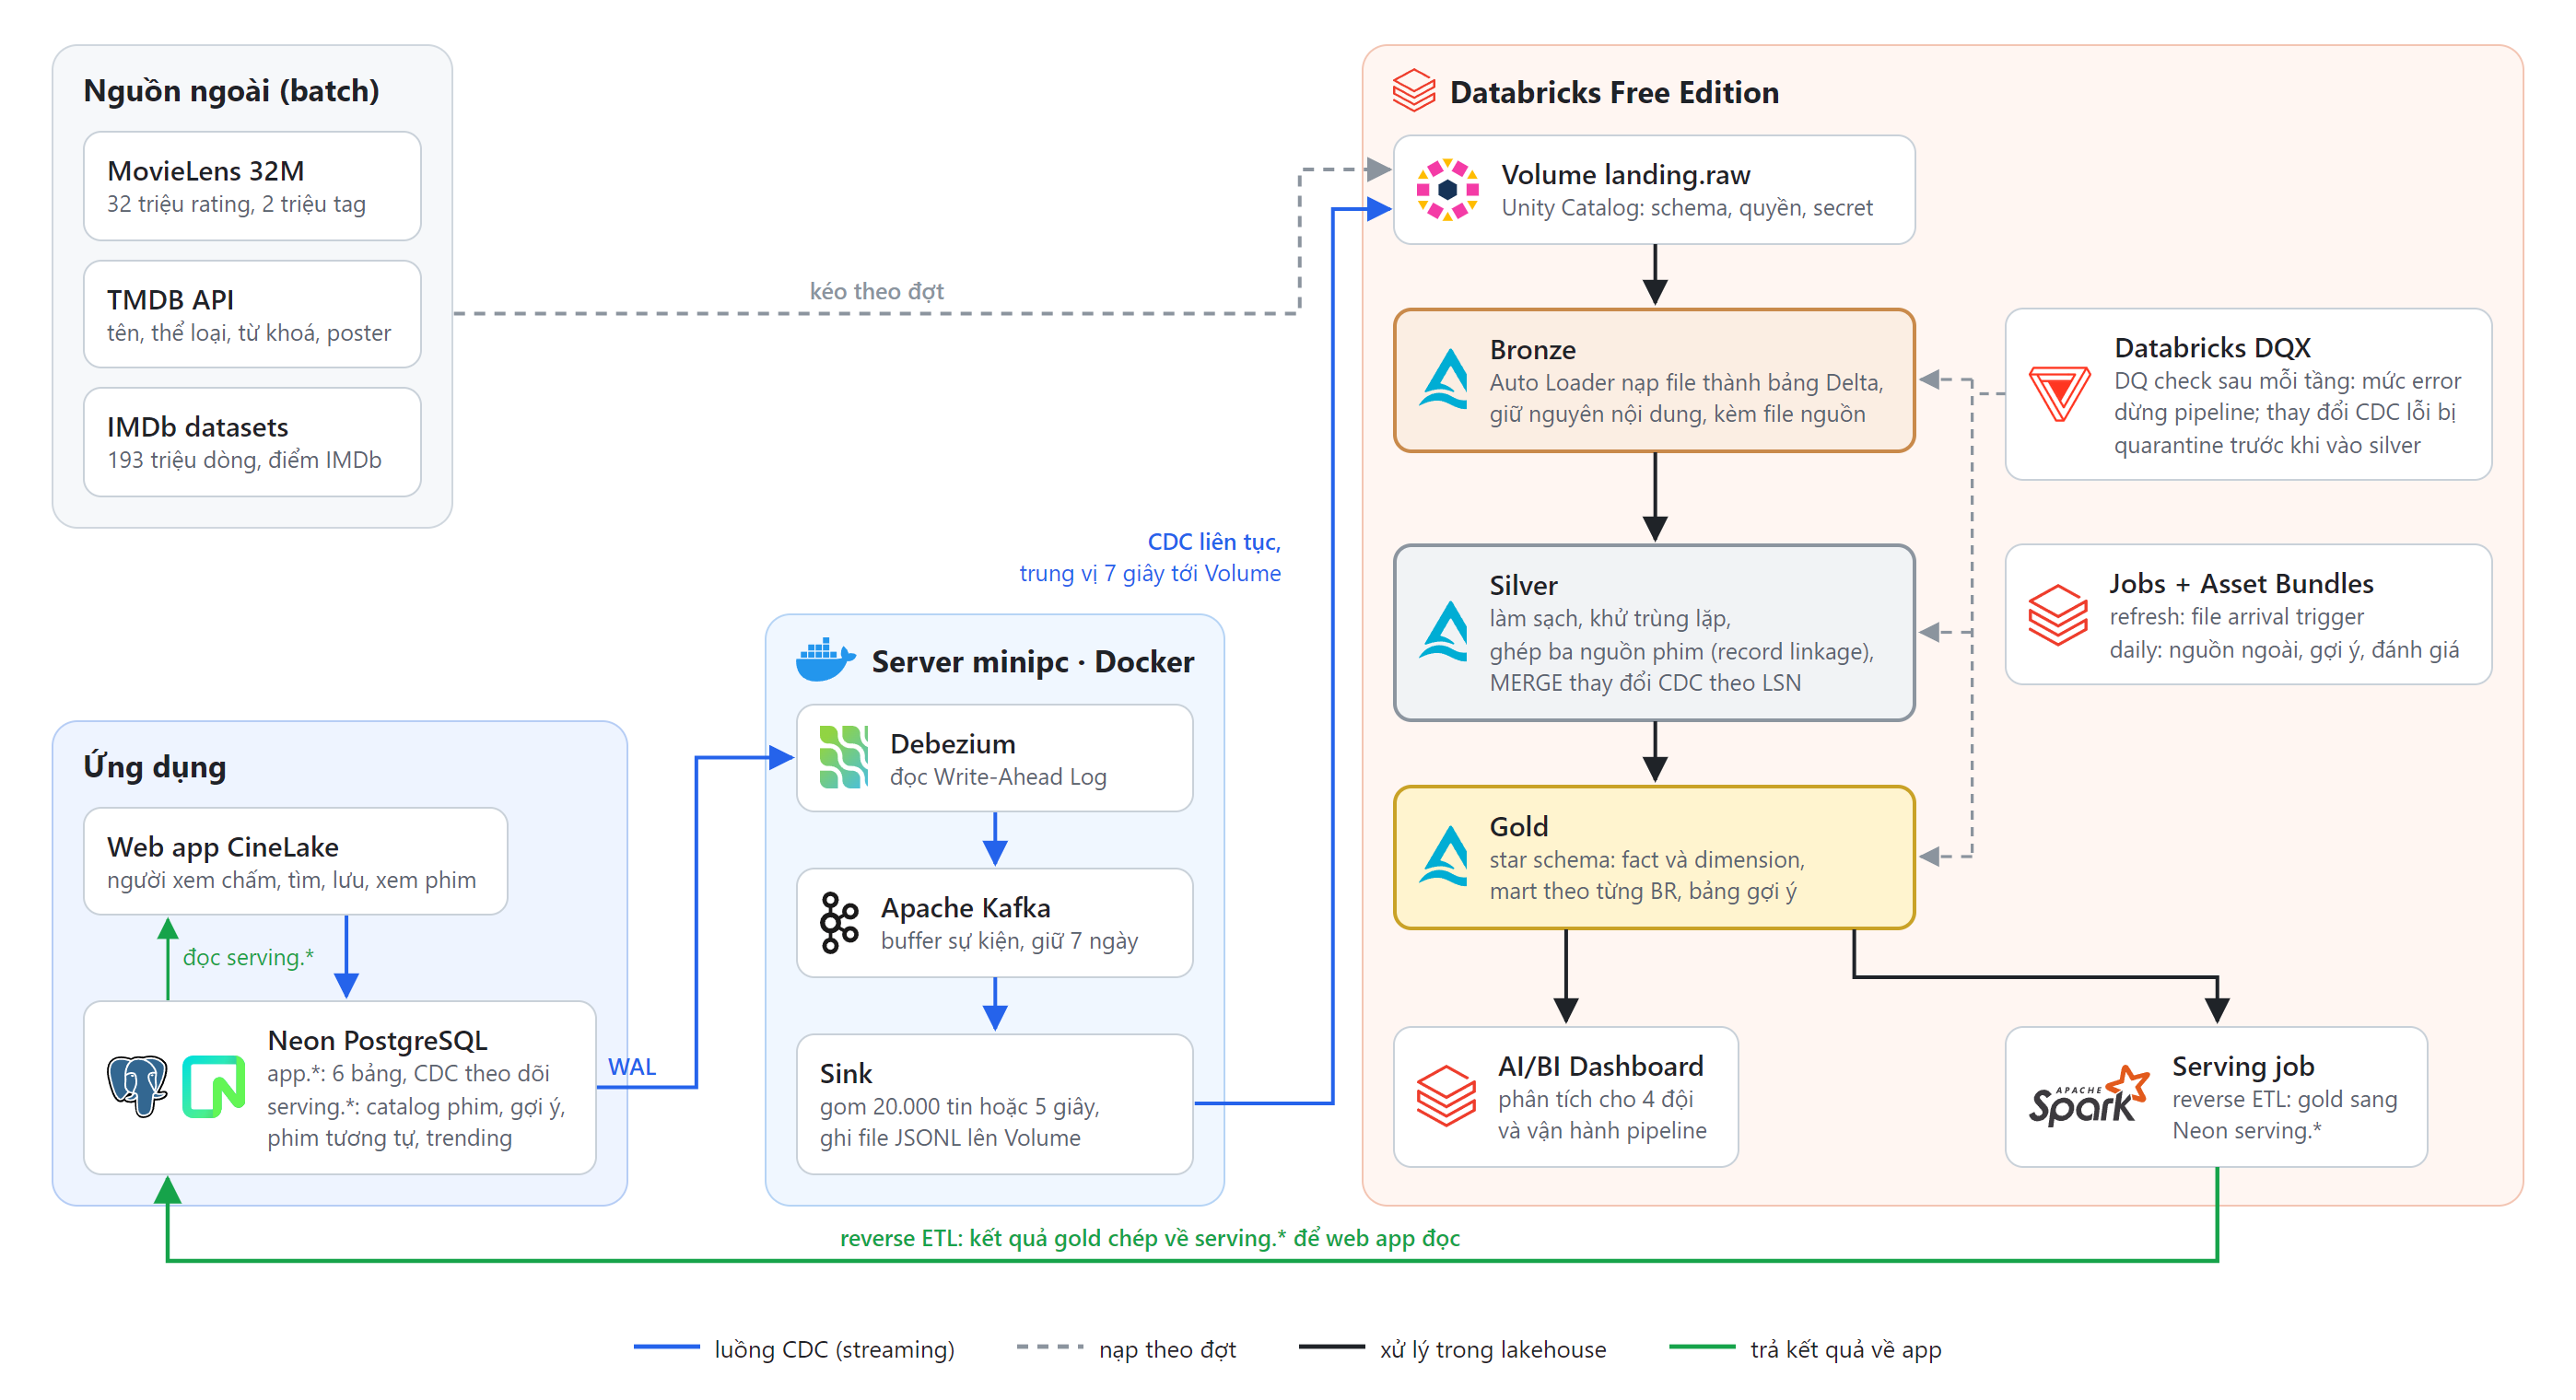
\includegraphics[width=\linewidth,height=0.84\textheight,keepaspectratio]{./images/hinh-01-kien-truc-tong-the.png}
\caption[Kiến trúc tổng thể của CineLake (mục 3.2)]{Kiến trúc tổng thể của CineLake: dữ liệu đi một vòng khép kín từ app đến CDC và lakehouse và quay về lại app.}
\label{fig:01}
\end{figure}

Bốn nguyên tắc thiết kế chi phối các quyết định bên dưới:

\begin{enumerate}
  \item \textbf{Mọi nguồn mô tả cùng người dùng, cùng phim, cùng dòng thời gian}, để các nguồn ghép được với nhau.
  \item \textbf{Dữ liệu nào thu về cũng phải được dùng}, và dữ liệu mô phỏng luôn tách được khỏi dữ liệu thật.
  \item \textbf{Idempotent:} một bước lỗi rồi chạy lại không làm mất hay nhân đôi dữ liệu.
  \item \textbf{Logic tách khỏi nền tảng:} phần biến đổi viết bằng PySpark thuần, nên kiểm thử được trên máy cá nhân và chuyển được sang nền tảng khác.
\end{enumerate}

\subsection{Thu thập dữ liệu}\label{sec:3.3}

Hai đường vào cùng kết thúc ở một vùng landing trên Volume, nơi giữ nguyên file gốc. Giữ file gốc giúp dựng lại toàn bộ lakehouse mà không phải tải lại nguồn. \newpage

\textbf{Đường batch cho external source}: \\
MovieLens được tải một lần. IMDb được tải lại tối đa mỗi tuần một lần, mỗi lần là một snapshot riêng. TMDB được gọi qua API với nhiều luồng song song và giới hạn tốc độ. Mỗi file nguồn được ghi số dòng vào một manifest; một DQ check so số dòng ở bronze với manifest này để phát hiện dữ liệu bị thiếu.


\textbf{Đường CDC cho database của app (Streaming)}:\\
Mỗi thay đổi trên app đi qua bốn chặng. \\
1. PostgreSQL ghi vào WAL \\
2. Debezium đọc WAL và đẩy vào Kafka, mỗi tin mang loại thao tác và vị trí LSN trong WAL \\
3 sink gom tin thành file (đủ 20.000 tin hoặc sau 5 giây) và đẩy lên Volume \\ 
4. Databricks nạp file vào bronze. Sink chỉ báo \textquotedbl{}đã đọc\textquotedbl{} cho Kafka sau khi file đã nằm trên Volume, nên nếu sink dừng giữa chừng thì lần sau sẽ gửi lại một đoạn, tuy nhiên có thể trùng, và silver sẽ loại sau đó\@.

\begin{figure}[H]
\centering
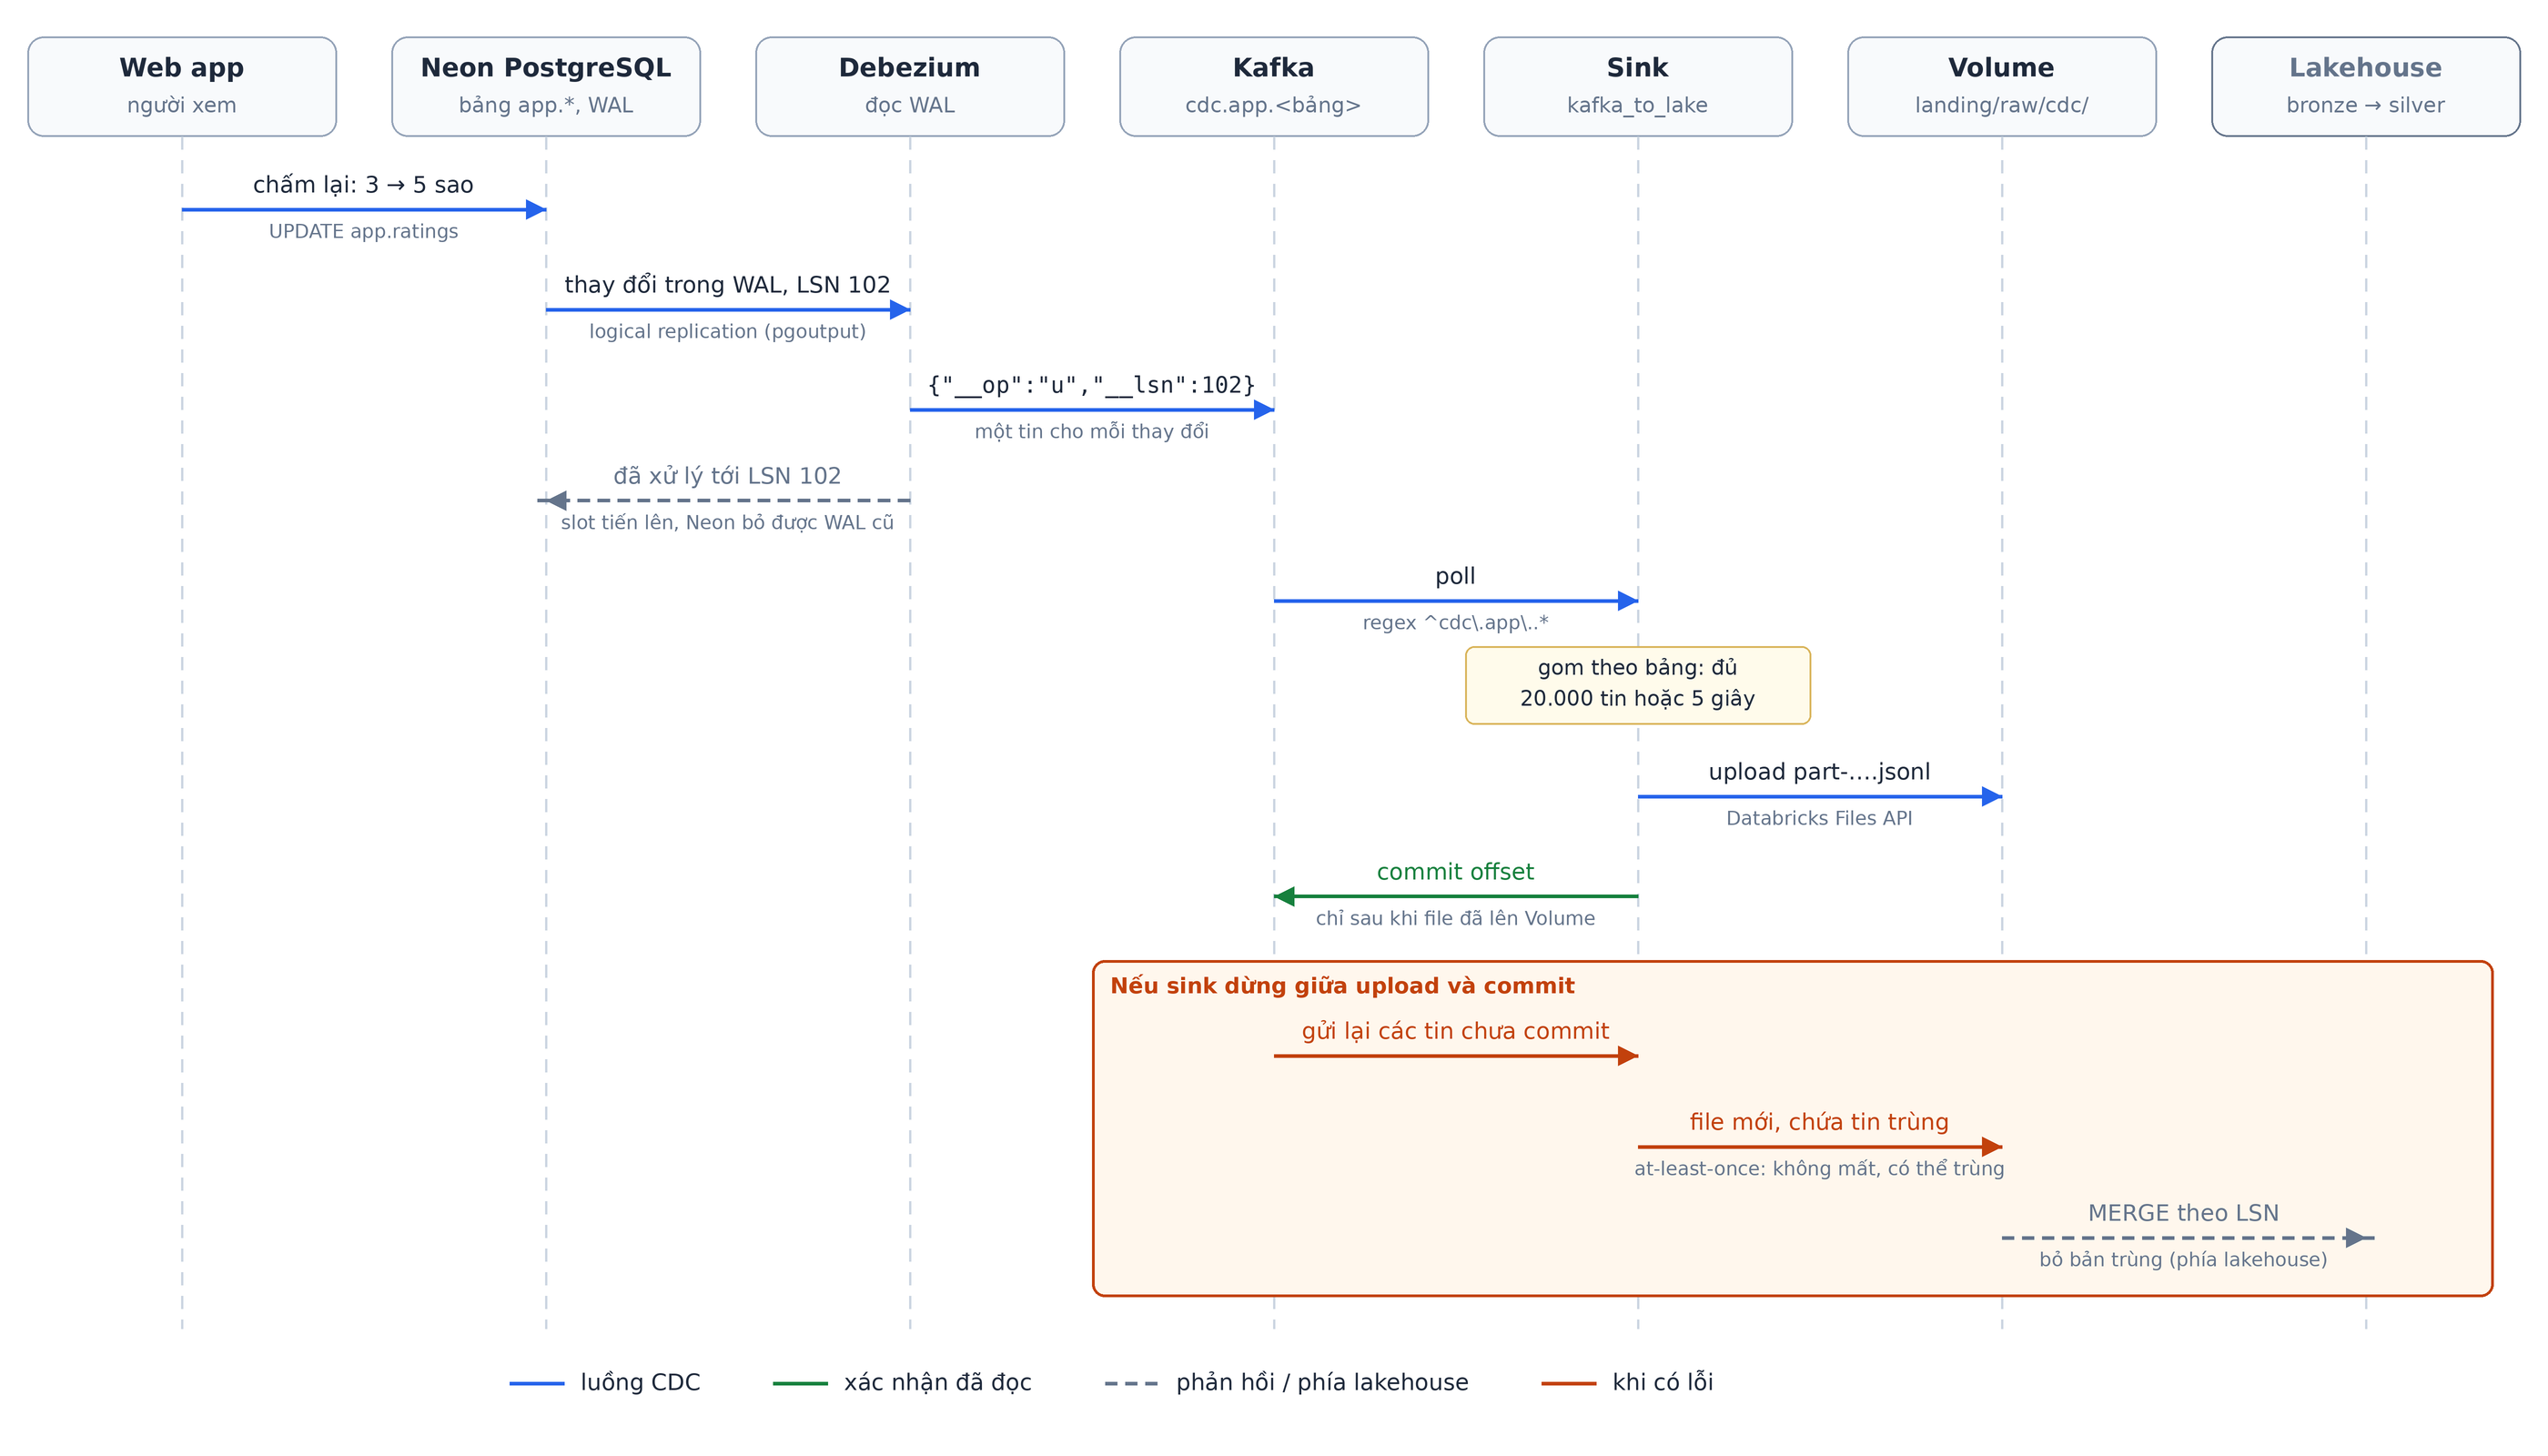
\includegraphics[width=\linewidth,height=0.84\textheight,keepaspectratio]{./images/hinh-02b-cdc-tuan-tu.png}
\caption[Trình tự một thay đổi đi qua đường CDC (mục 3.3)]{Trình tự một thay đổi đi qua đường CDC: sink chỉ commit offset sau khi file đã lên Volume}
\label{fig:cdc-seq}
\end{figure}


\textbf{Database của app trên Neon.} Database chia thành bốn schema, và chỉ schema \texttt{app} được CDC theo dõi (Bảng 8). Sáu bảng của schema \texttt{app} đều gắn với \texttt{user\dbsep{}id} (Hình 3). Số dòng đọc trực tiếp trên Neon ngày 08/11/2026:

\begin{itemize}
  \item \texttt{users} : 10.323, gồm 8.846 user MovieLens, 1.467 user do simulator tạo và 10 tài khoản app;
  \item \texttt{ratings} 882.895, \texttt{tags} 61.165, \texttt{watchlist} 26.082, \texttt{searches} 51.289;
  \item \texttt{events} 336.370, chỉ còn sự kiện từ 08/09 đến 07/11/2026, đúng 60 ngày mà cơ chế retention giữ lại; bản đầy đủ nằm ở \texttt{silver.\allowbreak{}events} (1.521.294 dòng).
\end{itemize}

\begingroup
\footnotesize
\setstretch{1.12}
\setlength{\tabcolsep}{4pt}
\renewcommand{\arraystretch}{1.18}
\setlength{\reporttablewidth}{\dimexpr\linewidth-10\tabcolsep\relax}
\begin{longtable}{@{}L{0.15\reporttablewidth} L{0.24\reporttablewidth} L{0.13\reporttablewidth} L{0.15\reporttablewidth} L{0.21\reporttablewidth} L{0.12\reporttablewidth}@{}}
\caption[Bốn schema của database app (mục 3.3)]{Bốn schema của database app trên Neon}\label{tab:08} \\
\toprule
\textbf{Schema} & \textbf{Chứa gì} & \textbf{Ai ghi} & \textbf{Ai đọc} & \textbf{CDC theo dõi} \\
\midrule
\endfirsthead
\toprule
\textbf{Schema} & \textbf{Nội dung} & \textbf{Thac tác ghi} & \textbf{Thac tác} & \textbf{CDC theo dõi}  \\
\midrule
\endhead
\midrule
\endfoot
\bottomrule
\endlastfoot
\texttt{app} & Hành vi người dùng & Web app & Web app, Debezium & Có \\
\texttt{serving} & Kết quả lakehouse tính sẵn & Job \texttt{cinelake\dbsep{}serving} & Web app & Không \\
\texttt{app\dbsep{}private} & Tài khoản, mật khẩu đã biến đổi, phiên đăng nhập; thêm ba bảng riêng của web app (ảnh phim, nguồn và biên nhận sự kiện) & Web app & Web app & Không  \\
\texttt{cdc\dbsep{}meta} & Bảng heartbeat & Debezium & Debezium & Có \\
\end{longtable}
\endgroup

\begin{figure}[H]
\centering
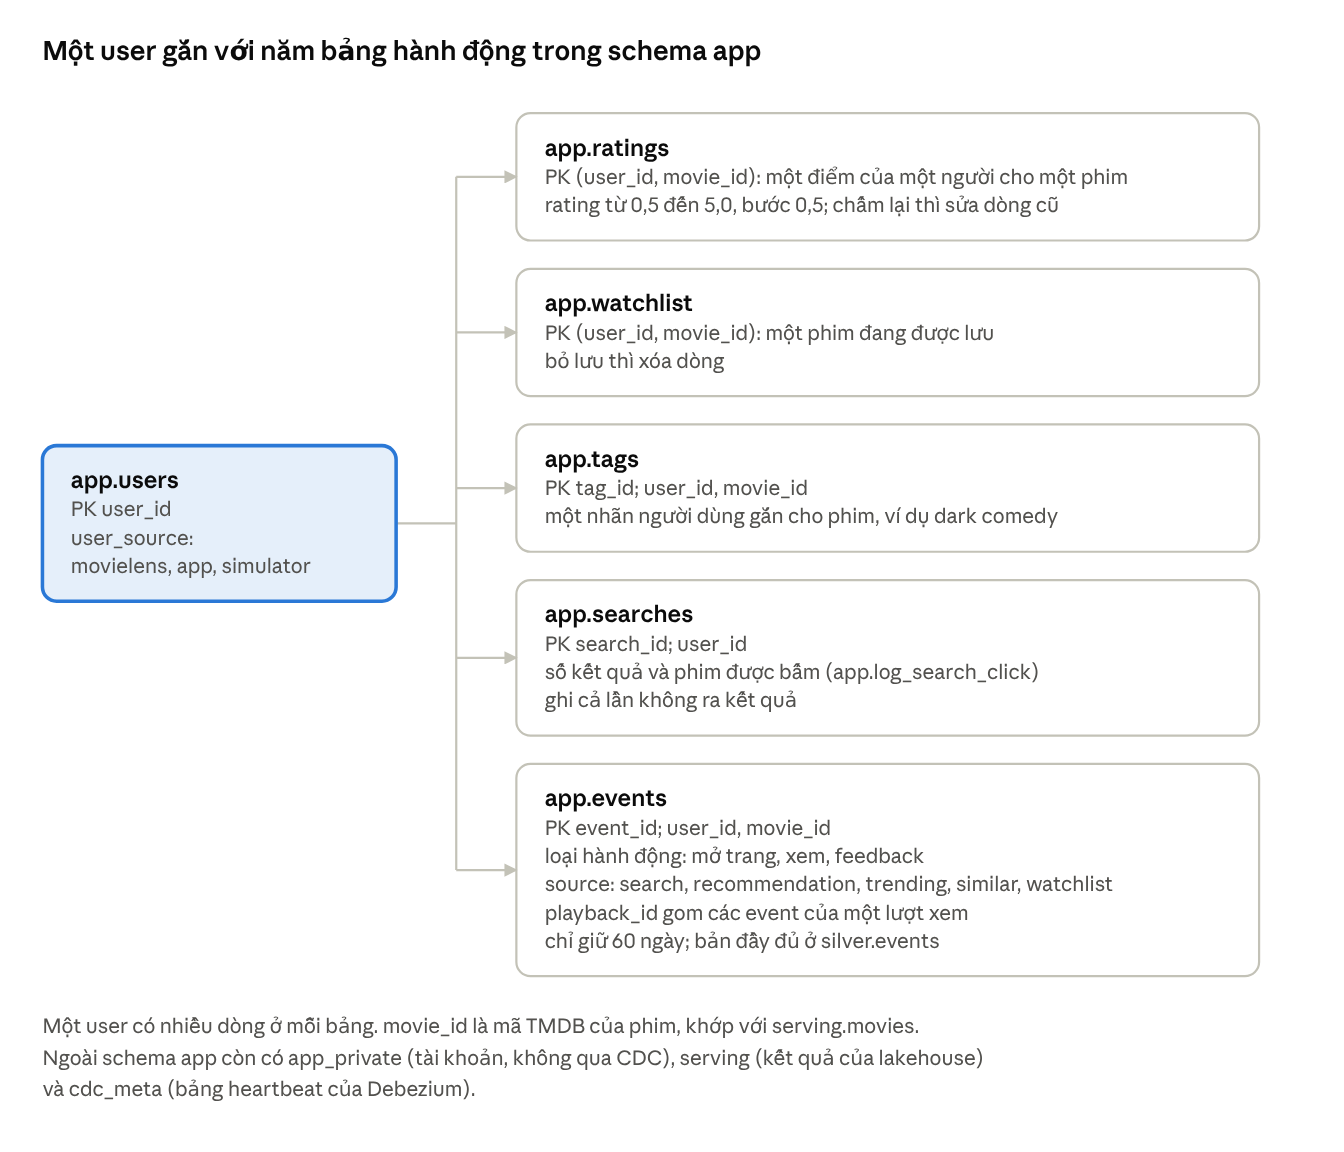
\includegraphics[width=\linewidth,height=0.84\textheight,keepaspectratio]{./images/hinh-02-erd-neon.png}
{\small\itshape ERD database app trên Neon \textperiodcentered{} 6 bảng schema app\par}
\caption[ERD database của app trên Neon (mục 3.3)]{ERD database của app trên Neon: một user gắn với năm bảng hành động.}
\label{fig:02}
\end{figure}

\subsection{Lakehouse: ba tầng bronze, silver, gold}\label{sec:3.4}

Lakehouse của CineLake theo kiến trúc medallion: dữ liệu đi qua ba tầng, mỗi tầng sạch hơn và gần nhu cầu kinh doanh hơn tầng trước. Bảng 9 tóm tắt vai trò từng tầng; các tiểu mục dưới đây nói rõ mỗi tầng chứa gì và được xử lý ra sao.

\begingroup
\small
\setstretch{1.12}
\setlength{\tabcolsep}{4pt}
\renewcommand{\arraystretch}{1.18}
\setlength{\reporttablewidth}{\dimexpr\linewidth-4\tabcolsep\relax}
\begin{longtable}{@{}L{0.15\reporttablewidth} L{0.42\reporttablewidth} L{0.43\reporttablewidth}@{}}
\caption[Ba tầng của lakehouse (mục 3.4)]{Ba tầng của lakehouse}\label{tab:09} \\
\toprule
\textbf{Tầng} & \textbf{Vai trò} & \textbf{Trong CineLake} \\
\midrule
\endfirsthead
\toprule
\textbf{Tầng} & \textbf{Vai trò} & \textbf{Trong CineLake} \\
\midrule
\endhead
\midrule
\endfoot
\bottomrule
\endlastfoot
Bronze & Bản gốc, không sửa nội dung, kèm thông tin file nguồn & 11 bảng, 233,1 triệu dòng \\
Silver & Thực thể đã làm sạch: đúng kiểu, không trùng, đã qua record linkage & 83.082 phim, 202.425 user, 32.002.850 rating \\
Gold & Bảng trả lời câu hỏi: star schema, mart cho từng BR, gợi ý & 21 bảng, mô tả bên dưới \\
\end{longtable}
\endgroup

Tách tầng như vậy giúp một dòng lỗi không làm hỏng cả đợt nạp, và silver luôn dựng lại được từ bronze khi logic làm sạch thay đổi. Mỗi tầng nằm trong một schema riêng của Unity Catalog ( \texttt{bronze} , \texttt{silver} , \texttt{gold} ).

\subsubsection*{Bronze: nhận file vào bảng}

Bronze sao chép file ở landing vào bảng Delta mà không sửa nội dung: mọi cột là chữ (string). Mỗi bảng có thêm hai cột truy vết: \texttt{\dbsep{}source\dbsep{}file} cho biết dòng đến từ file nào, \texttt{\dbsep{}ingested\dbsep{}at} cho biết nạp lúc nào.

Tầng này có 11 bảng, 233,1 triệu dòng, chia theo nguồn:

\begin{itemize}
  \item \textbf{MovieLens (4 bảng):} phim, rating, tag và bảng nối mã MovieLens với mã TMDB và IMDb. Riêng rating có 32 triệu dòng.
  \item \textbf{TMDB (1 bảng):} phản hồi API cho từng phim, giữ nguyên JSON.
  \item \textbf{IMDb (5 bảng):} điểm, thông tin phim, người tham gia từng phim, thông tin người và tên phim theo quốc gia. Đây là 193 triệu dòng, chiếm gần hết tầng bronze.
  \item \textbf{Database của app (1 bảng):} \texttt{app\dbsep{}cdc\dbsep{}changes} chứa thay đổi của cả 6 bảng app, khoảng 5,6 triệu dòng. Gom chung một bảng để giữ được thứ tự LSN giữa các bảng. Các cột tên bảng, loại thay đổi, LSN, thời điểm nguồn và cờ xoá được tách ra; dòng JSON gốc giữ ở cột \texttt{payload} .
\end{itemize}

Bronze được nạp bằng Auto Loader như mô tả ở mục 3.1: phần CDC chạy mỗi vòng, phần nguồn ngoài chỉ chạy trong job daily và job khởi tạo. Danh sách đầy đủ ở Phụ lục E (Bảng 26).

\subsubsection*{Silver: làm sạch và chuẩn hoá}

Silver đọc bronze, ép đúng kiểu, bỏ trùng và tách thành bảng theo thực thể (phim, người, user, rating). Khoá phim toàn hệ thống là \texttt{movie\dbsep{}id} , chính là mã TMDB. Giá trị không ép được kiểu thành NULL để DQ check bắt được.

Tầng này có 14 bảng, thuộc hai nhóm xử lý khác nhau:

\begin{itemize}
  \item \textbf{Danh mục phim (5 bảng, 83.082 phim):} ghép từ MovieLens, TMDB và IMDb, gồm bảng phim, bảng nối mã, người tham gia, thông tin người và tên phim (có tên tiếng Việt). Nhóm này chỉ dựng lại khi có dữ liệu batch mới.
  \item \textbf{Dữ liệu từ app (9 bảng, 202.425 user, 32.002.850 rating):} gồm trạng thái hiện tại (user, rating, tag, Danh sách yêu thích, tìm kiếm, sự kiện), lịch sử từng lần đổi rating và Danh sách yêu thích (phục vụ kiểm tra và BR8) và một bảng quarantine chứa thay đổi lỗi. Nhóm này cập nhật mỗi vòng bằng MERGE.
\end{itemize}

Hình 4 cho thấy hai cụm thực thể của silver: danh mục phim nối nhau qua \texttt{movie\dbsep{}id} (mã TMDB), còn các bảng dữ liệu từ app nối với nhau qua \texttt{user\dbsep{}id} và \texttt{movie\dbsep{}id} . Danh sách bảng kèm số dòng ở Phụ lục E (Bảng 27).

\begin{figure}[H]
\centering
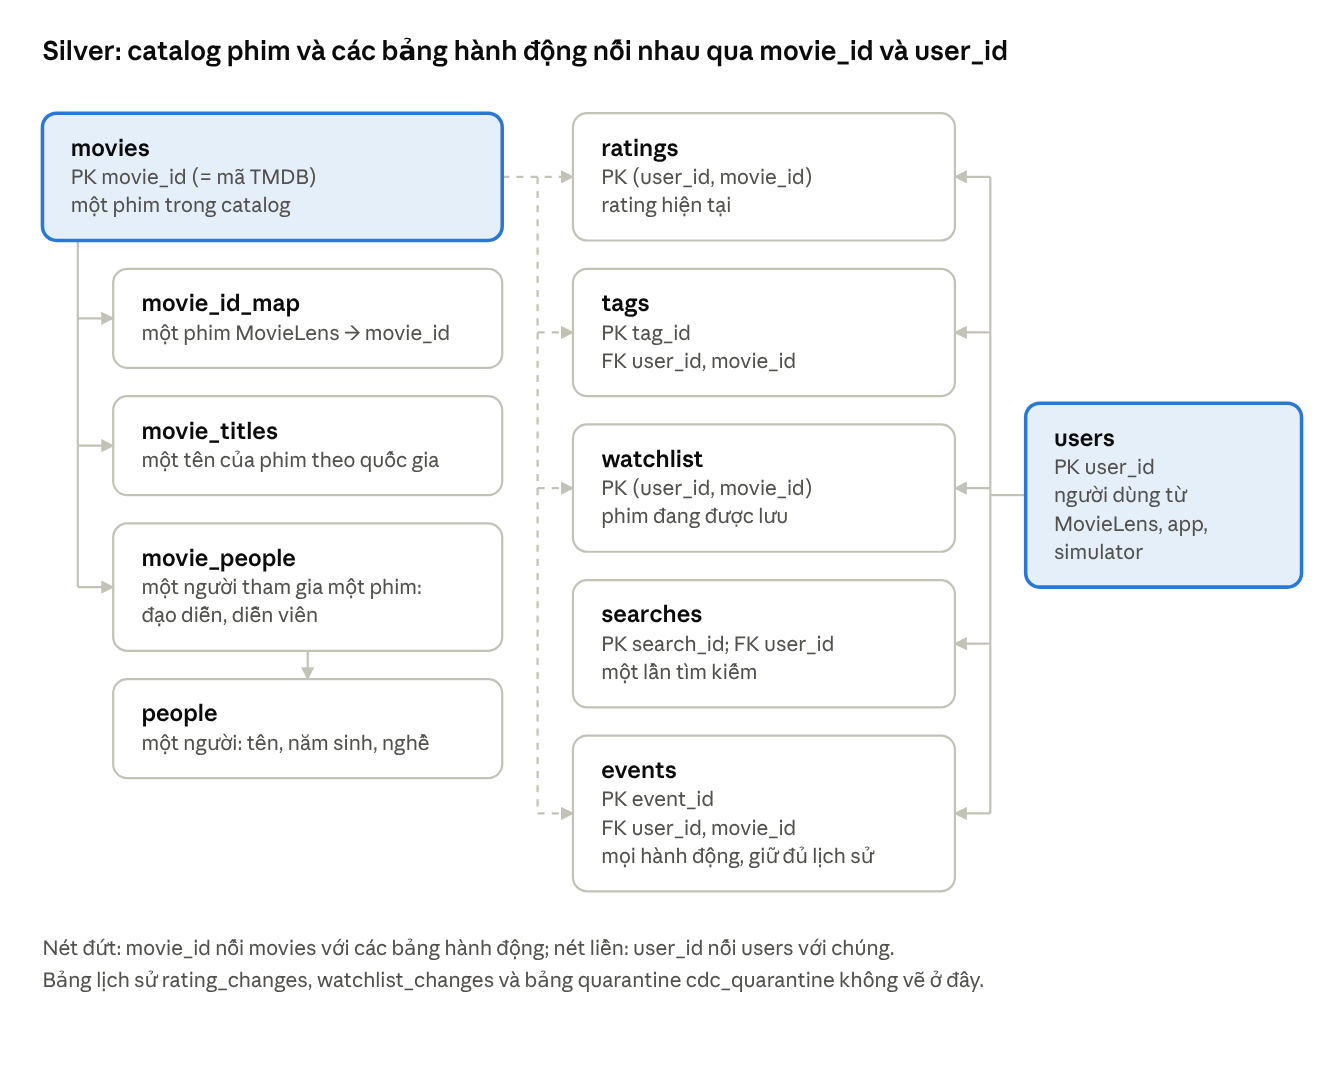
\includegraphics[width=\linewidth,height=0.84\textheight,keepaspectratio]{./images/hinh-03-mo-hinh-silver.png}
{\small\itshape Mô hình thực thể silver \textperiodcentered{} catalog phim và bảng hành động\par}
\caption[Mô hình thực thể của silver (mục 3.4)]{Mô hình thực thể của silver: catalog phim và các bảng hành động.}
\label{fig:03}
\end{figure}

\textbf{Record linkage.} Bước khó nhất của silver là ghép ba nguồn về cùng một mã phim (mã TMDB). Pipeline ghi lại lý do cho mỗi phim không ghép được, và kết quả là catalog 83.082 phim giữ được 99,74\% số rating.

IMDb được lọc sớm: chỉ giữ 1,9\% số dòng, là phần thuộc phim có trong catalog, nhờ đó các bước sau nhẹ hơn nhiều.

\textbf{Áp thay đổi từ app vào silver.} Bronze ghi lại từng lần đổi, còn silver chỉ giữ trạng thái cuối.

Pipeline dùng lệnh MERGE của Delta với một quy tắc: một thay đổi chỉ được áp nếu nó mới hơn (có LSN lớn hơn) dữ liệu đang có. Nhờ quy tắc này, tin gửi lại hay đến sai thứ tự đều vô hại, và chạy lại bao nhiêu lần cũng cho cùng kết quả (tính idempotent).

\begin{quote}
\textbf{Ví dụ: một lần chấm lại đi qua pipeline.} Một user chấm một phim 4,5 sao, rồi sửa thành 3 sao; sink dừng giữa chừng nên tin đầu tiên bị gửi lại. Gọi thứ tự của các thay đổi là L1 \textless{} L2 \textless{} L3.
\end{quote}

\begingroup
\small
\setstretch{1.12}
\setlength{\tabcolsep}{4pt}
\renewcommand{\arraystretch}{1.18}
\setlength{\reporttablewidth}{\dimexpr\linewidth-6\tabcolsep\relax}
\begin{longtable}{@{}L{0.13\reporttablewidth} L{0.25\reporttablewidth} L{0.27\reporttablewidth} L{0.35\reporttablewidth}@{}}
\caption[Một lần chấm lại đi qua pipeline (mục 3.4)]{Một lần chấm lại đi qua pipeline}\label{tab:10} \\
\toprule
\textbf{Bước} & \textbf{Bronze nhận} & \textbf{Silver sau MERGE} & \textbf{Vì sao} \\
\midrule
\endfirsthead
\toprule
\textbf{Bước} & \textbf{Bronze nhận} & \textbf{Silver sau MERGE} & \textbf{Vì sao} \\
\midrule
\endhead
\midrule
\endfoot
\bottomrule
\endlastfoot
1 & Thêm: 4,5 sao, L1 & 4,5 sao (L1) & Chưa có dòng nào: thêm mới \\
2 & Sửa: 3 sao, L2 & 3 sao (L2) & L2 mới hơn L1: cập nhật \\
3 & Thêm: 4,5 sao, L1 (gửi lại) & 3 sao (L2) & L1 cũ hơn L2: bỏ qua \\
4 & Xoá: L3 & Không còn dòng & Xoá; nếu user có rating lịch sử cho phim này thì rating đó được trả lại \\
\end{longtable}
\endgroup

Bronze có bốn dòng, silver luôn chỉ có một kết quả đúng; lịch sử cả hai lần chấm vẫn được giữ riêng để kiểm tra về sau.

\subsubsection*{Gold: trả lời câu hỏi kinh doanh}

\textbf{Star schema.} Tầng gold được mô hình hoá theo star schema của Kimball: fact ghi sự kiện có số đo, dimension mô tả đối tượng (phim, user, ngày).

\textbf{Accumulating snapshot.} Hai fact xem phim và lưu phim dùng dạng này: mỗi lượt xem hay mỗi lần lưu là một dòng, được cập nhật dần khi các mốc tiếp theo xảy ra (xem hết; được xem, được chấm, bị bỏ), dựa theo yêu cầu của BR6 và BR8.

\textbf{Mart.} Mỗi BR trên dashboard có mart riêng, tính sẵn theo một mức cố định và chỉ đọc bảng gold: các fact, thêm dimension hoặc \texttt{mart\dbsep{}movie\dbsep{}catalog} khi cần thông tin phim hay user. Gold có 21 bảng: 3 dimension, 7 fact, 9 mart và 2 bảng gợi ý (Hình 5). Các fact được mô tả ở Bảng 11 bên dưới, mart và bảng gợi ý ở Phụ lục E (Bảng 28).

\begin{figure}[H]
\centering
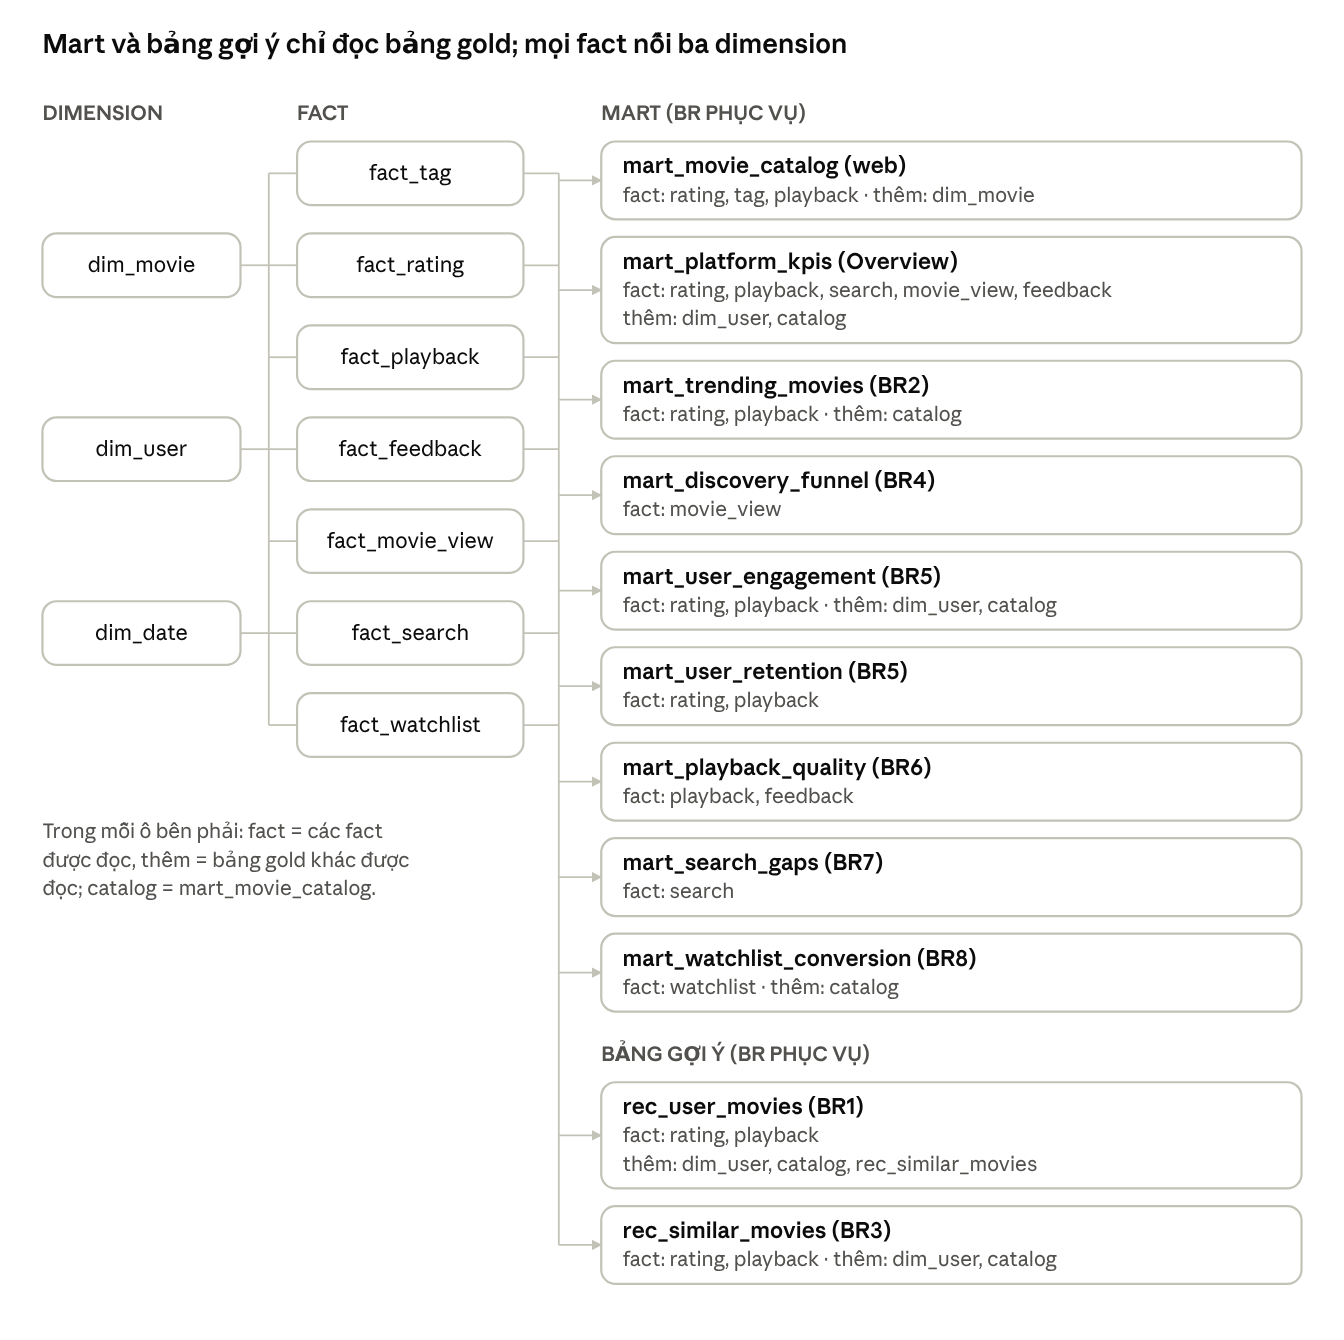
\includegraphics[width=\linewidth,height=0.84\textheight,keepaspectratio]{./images/hinh-04-star-schema-gold.png}
{\small\itshape Star schema gold \textperiodcentered{} fact, dimension, mart và bảng gợi ý\par}
\caption[Star schema của tầng gold (mục 3.4)]{Star schema của tầng gold, các mart và bảng gợi ý đọc từ nó.}
\label{fig:04}
\end{figure}

\begingroup
\small
\setstretch{1.12}
\setlength{\tabcolsep}{4pt}
\renewcommand{\arraystretch}{1.18}
\setlength{\reporttablewidth}{\dimexpr\linewidth-4\tabcolsep\relax}
\begin{longtable}{@{}L{0.26\reporttablewidth} L{0.44\reporttablewidth} L{0.30\reporttablewidth}@{}}
\caption[Các bảng fact và dimension của tầng gold (mục 3.4)]{Các bảng fact và dimension của tầng gold}\label{tab:11} \\
\toprule
\textbf{Bảng} & \textbf{Nội dung} & \textbf{Số dòng (08/11)} \\
\midrule
\endfirsthead
\toprule
\textbf{Bảng} & \textbf{Nội dung} & \textbf{Số dòng (08/11)} \\
\midrule
\endhead
\midrule
\endfoot
\bottomrule
\endlastfoot
\texttt{fact\dbsep{}rating} & Cặp user--movie, lưu điểm đánh giá hiện tại, thời điểm chấm và nguồn dữ liệu. & 32.002.850 \\
\texttt{fact\dbsep{}tag} & Gắn thẻ cho phim, gồm người gắn, nội dung thẻ, khoá thẻ dùng để nhóm, thời điểm và nguồn dữ liệu. & 1.972.972 \\
\texttt{fact\dbsep{}movie\dbsep{}view} & Một lần mở trang phim, gồm user, session, thời điểm, kênh khám phá, vị trí phim và ý định mở; kèm các flag ghi nhận lượt mở dẫn tới xem, xem hết hoặc chấm điểm. & 1.145.626 \\
\texttt{fact\dbsep{}search} & Một lượt tìm kiếm, lưu chuỗi gốc và chuẩn hoá, bộ lọc thể loại, thời điểm, số kết quả và phim được bấm nếu có. & 51.289 \\
\texttt{fact\dbsep{}playback} & Một lượt phát phim, tổng hợp các sự kiện của player thành trạng thái, thời lượng và tỉ lệ xem, thiết bị, phiên bản player, độ trễ khi phát, buffering và lỗi. & 48.460 \\
\texttt{fact\dbsep{}watchlist} & Một cặp user--movie được lưu, theo dõi thời điểm lưu, xem, chấm và bỏ; kèm trạng thái, cờ xem hết và số ngày từ lúc lưu tới xem hoặc chấm. & 26.114 \\
\texttt{fact\dbsep{}feedback} & Một phản hồi về playback, gồm loại phản hồi, thời điểm, người dùng, phim, thiết bị và phiên bản player; liên kết với lượt phát gần nhất trong 24 giờ. & 1.847 \\
\texttt{dim\dbsep{}movie} & Một phim, gồm mã liên kết MovieLens/TMDB/IMDb, tên, thể loại, năm phát hành, thời lượng, điểm TMDB/IMDb, từ khoá, đạo diễn, diễn viên và cờ còn trong catalog. Có một phim TMDB đã gỡ nhưng vẫn còn hoạt động tham chiếu. & 83.083 \\
\texttt{dim\dbsep{}user} & Một tài khoản, gồm nguồn MovieLens/simulator/app, cờ tài khoản mô phỏng, thông tin hồ sơ và cờ hồ sơ sinh tự động, thời điểm xuất hiện đầu tiên và hoạt động gần nhất. & 202.425 \\
\texttt{dim\dbsep{}date} & Một ngày, gồm khoá ngày, thứ, tuần, tháng, quý, năm và các cờ cuối tuần, sau thời điểm ra mắt; dùng để nhóm và lọc các fact theo lịch. & 10.534 \\
\end{longtable}
\endgroup

\subsection{Kiểm soát chất lượng dữ liệu}\label{sec:3.5}

Nguyên tắc là dữ liệu sai phải bị chặn trước khi tới người dùng. Nhóm áp dụng mô hình write--audit--publish: ghi dữ liệu, kiểm tra, rồi mới công bố. Nếu một rule mức error không đạt, job dừng, các tầng sau không chạy, và web app tiếp tục dùng kết quả đúng gần nhất.

Các rule nằm trong file YAML của DQX (mục 3.1); mỗi rule chạy theo một trong ba chế độ:

\begingroup
\small
\setstretch{1.12}
\setlength{\tabcolsep}{4pt}
\renewcommand{\arraystretch}{1.18}
\setlength{\reporttablewidth}{\dimexpr\linewidth-4\tabcolsep\relax}
\begin{longtable}{@{}L{0.20\reporttablewidth} L{0.39\reporttablewidth} L{0.41\reporttablewidth}@{}}
\caption[Các mức độ kiểm soát chất lượng (mục 3.5)]{Các mức độ kiểm soát chất lượng}\label{tab:12} \\
\toprule
\textbf{Chế độ} & \textbf{Áp dụng} & \textbf{Khi vi phạm} \\
\midrule
\endfirsthead
\toprule
\textbf{Chế độ} & \textbf{Áp dụng} & \textbf{Khi vi phạm} \\
\midrule
\endhead
\midrule
\endfoot
\bottomrule
\endlastfoot
Quarantine & Từng thay đổi CDC, trước khi áp vào silver (20 quarantine rule) & Dòng sai vào bảng quarantine kèm tên rule, dòng đúng đi tiếp \\
Flag & Catalog phim & Dòng vẫn giữ, kèm cảnh báo \\
Giám sát & Các bảng còn lại, sau khi ghi (45 DQ check) & Mức error dừng job, mức warn chỉ cảnh báo \\
\end{longtable}
\endgroup

45 DQ check được xếp theo 6 chiều chất lượng của DAMA (đầy đủ, hợp lệ, nhất quán, duy nhất, toàn vẹn tham chiếu, chính xác) và được chạy sau từng tầng; kết quả mỗi lần chạy được lưu lại để dashboard vận hành hiển thị. Tổng cộng 65 rule (45 DQ check và 20 quarantine rule) không phải 65 loại kiểm tra khác nhau: nhiều rule là cùng một kiểm tra áp cho từng bảng, ví dụ LSN không rỗng và loại thay đổi hợp lệ cho cả 6 bảng app, hay số dòng fact khớp silver cho 6 bảng fact. Mục 5.1 trình bày các check và kết quả.

\subsection{Hệ gợi ý và đưa kết quả về app}\label{sec:3.6}

\textbf{Hệ gợi ý (BR1, BR3)} có hai lớp, học từ cách Netflix tách tầng offline và online:

\begin{itemize}
  \item \textbf{Lớp offline trên Databricks.} Phim tương tự dùng item-item collaborative filtering: nếu nhiều người cùng thích hai phim (chấm từ 4 sao hoặc xem hết) thì hai phim giống nhau, đo bằng cosine. Cách này phủ 16.684 phim; 65.812 phim ít người chấm còn lại được so theo nội dung (thể loại, từ khoá, đạo diễn và diễn viên, tag), nên 99,3\% catalog có phim tương tự.

  Gợi ý cá nhân lấy các phim user đã thích, cộng điểm các phim tương tự, bỏ phim đã xem, rồi chọn 10 phim kèm lý do \textquotedbl{}because you liked X\textquotedbl{}. Nhóm chọn item-item CF thay vì matrix factorization (ALS) chính vì giải thích được lý do này cho người xem.
  \item \textbf{Lớp online trong PostgreSQL.} Một hàm SQL trộn 10 gợi ý offline với các hành động trong 7 ngày gần nhất (chấm điểm, xem hết, lưu phim, mở phim), hành động càng mới càng nặng ký. Nhờ vậy, người xem vừa chấm một phim là thấy gợi ý đổi ngay, không phải chờ vòng lakehouse tiếp theo.
\end{itemize}

\textbf{Đưa kết quả về app (reverse ETL).} Bước serving chép năm bảng từ gold về PostgreSQL: catalog phim, gợi ý cá nhân, phim tương tự, Top 10 tuần và rating cũ của user. Đây là bước duy nhất ghi ra ngoài lakehouse, chỉ chạy khi mọi tầng trước đã đạt kiểm tra chất lượng. Dữ liệu được chép vào bảng tạm rồi đổi tên trong một giao dịch, nên web app không bao giờ đọc phải bảng đang ghi dở.

\textbf{Đường đi của dữ liệu cho từng BR.} Bảng dưới nối mỗi BR với nguồn dữ liệu, bảng gold được dùng và nơi kết quả xuất hiện.

\begingroup
\small
\setstretch{1.12}
\setlength{\tabcolsep}{4pt}
\renewcommand{\arraystretch}{1.18}
\setlength{\reporttablewidth}{\dimexpr\linewidth-6\tabcolsep\relax}
\begin{longtable}{@{}L{0.08\reporttablewidth} L{0.28\reporttablewidth} L{0.39\reporttablewidth} L{0.25\reporttablewidth}@{}}
\caption[Đường đi của dữ liệu cho từng BR (mục 3.6)]{Đường đi của dữ liệu cho từng BR}\label{tab:13} \\
\toprule
\textbf{BR} & \textbf{Nguồn} & \textbf{Bảng gold} & \textbf{Nơi dùng kết quả} \\
\midrule
\endfirsthead
\toprule
\textbf{BR} & \textbf{Nguồn} & \textbf{Bảng gold} & \textbf{Nơi dùng kết quả} \\
\midrule
\endhead
\midrule
\endfoot
\bottomrule
\endlastfoot
BR1 & Rating MovieLens, rating và lượt xem mới từ app (CDC) & Rating, Xem phim; bảng gợi ý cá nhân & Web: \textquotedbl{}Picked for you\textquotedbl{}, qua PostgreSQL \\
BR2 & Rating và lượt xem từ app (CDC) & Rating, Xem phim; mart\dbsep{}trending\dbsep{}movies (Top 10 tuần) & Web: \textquotedbl{}Top 10 this week\textquotedbl{}, qua PostgreSQL \\
BR3 & Rating và tag MovieLens, TMDB, IMDb & Rating, Xem phim, Tag, dimension phim; bảng phim tương tự & Web: \textquotedbl{}More like X\textquotedbl{}, qua PostgreSQL \\
BR4 & Lượt mở trang phim, lượt xem từ app (CDC) & Mở trang phim, Xem phim; mart\dbsep{}discovery\dbsep{}funnel & Dashboard, trang Product \\
BR5 & Hoạt động của user từ MovieLens và app (CDC) & Các fact hành động, dimension user; mart\dbsep{}user\dbsep{}engagement, mart\dbsep{}user\dbsep{}retention & Dashboard, trang Marketing \\
BR6 & Sự kiện player và phản hồi từ app (CDC) & Xem phim, Phản hồi; mart\dbsep{}playback\dbsep{}quality & Dashboard, trang Playback \\
BR7 & Lượt tìm kiếm từ app (CDC), catalog từ TMDB & Tìm kiếm; mart\dbsep{}search\dbsep{}gaps & Dashboard, trang Content; web trả 0 kết quả \\
BR8 & Lần lưu, xem và bỏ khỏi Danh sách yêu thích từ app (CDC) & Lưu phim; mart\dbsep{}watchlist\dbsep{}conversion & Dashboard, trang Marketing; web: Danh sách yêu thích \\
\end{longtable}
\endgroup

\subsection{Vận hành và bảo mật}\label{sec:3.7}

\textbf{Điều phối.} Mỗi tầng là một job (nạp, silver, gold, serving); một job tổng nối chúng theo thứ tự, job sau chỉ chạy khi job trước thành công. Job tổng dùng file arrival trigger: Databricks theo dõi thư mục CDC và chạy một vòng khi có file mới. Một job daily làm thêm các việc nặng: kéo nguồn ngoài, tính lại phim tương tự, đánh giá gợi ý.

Như vậy, thu thập là streaming thật (Debezium, Kafka và sink chạy liên tục), lakehouse xử lý theo micro-batch, còn phản hồi real-time nằm ở PostgreSQL. Thời gian xử lý một vòng được đo ở mục 5.2.

Dashboard vận hành cho đội dữ liệu biết dữ liệu có đang tới không (Hình 6), và một thay đổi đã đi tới tầng nào (Hình 7).

\begin{figure}[H]
\centering
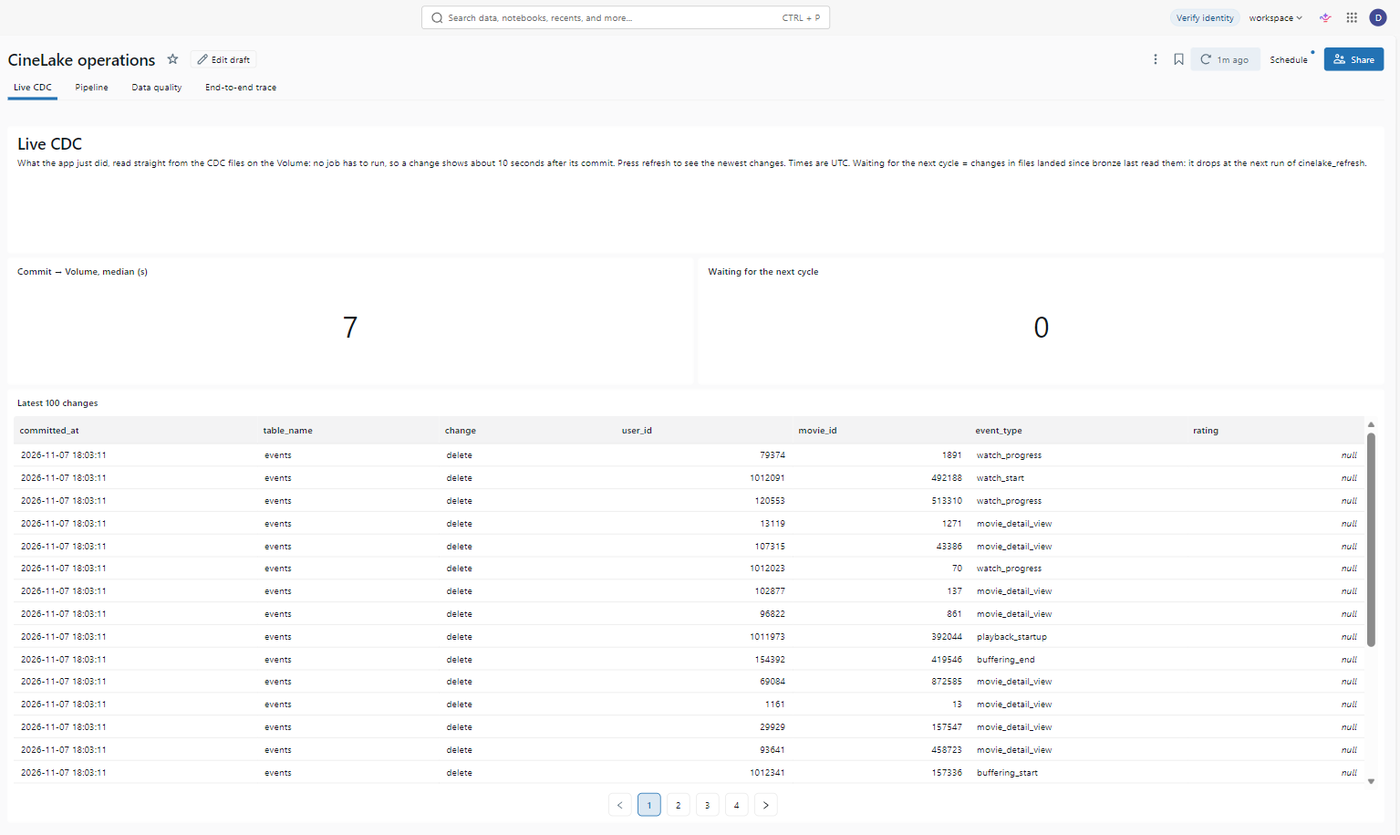
\includegraphics[width=\linewidth,height=0.84\textheight,keepaspectratio]{./images/hinh-05-live-cdc.png}
\caption[Dashboard vận hành, trang Live CDC (mục 3.7)]{Trang Live CDC (08/11/2026): thay đổi vừa xảy ra trên app và độ trễ từ lúc ghi tới lúc file lên Volume.}
\label{fig:05}
\end{figure}

\begin{figure}[H]
\centering
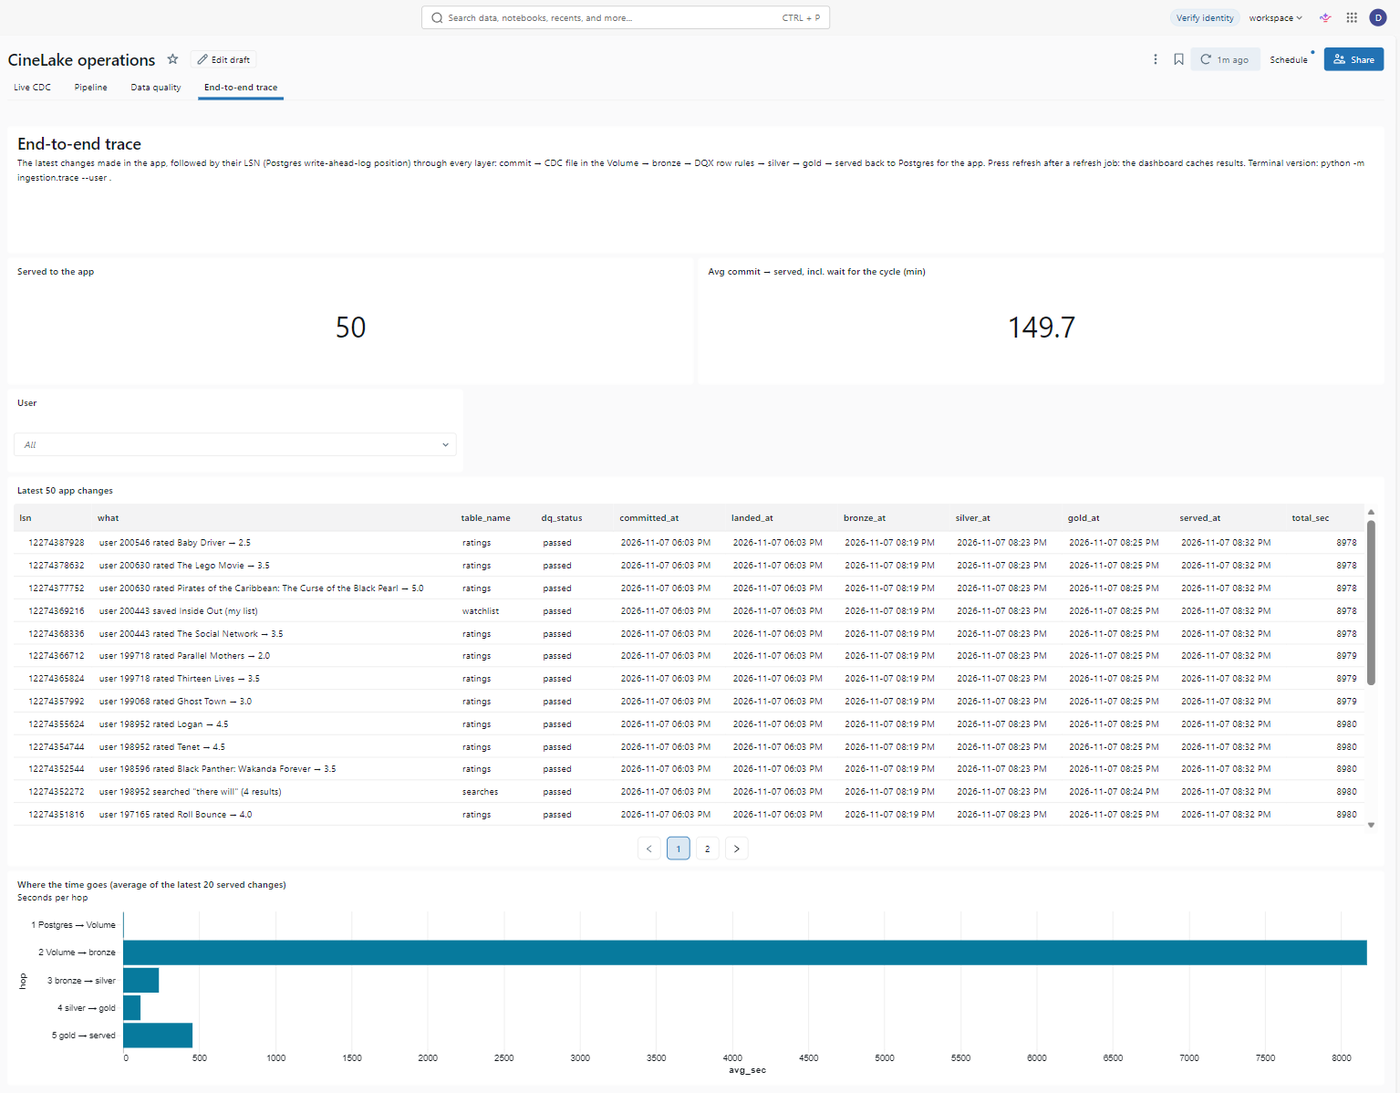
\includegraphics[width=\linewidth,height=0.84\textheight,keepaspectratio]{./images/hinh-06-end-to-end-trace.png}
\caption[Dashboard vận hành, trang End-to-end trace (mục 3.7)]{Trang End-to-end trace (08/11/2026): mỗi dòng là một thay đổi, kèm thời điểm qua từng tầng.}
\label{fig:06}
\end{figure}

\textbf{Xử lý lỗi.} Pipeline được thiết kế để các lỗi thường gặp không làm sai dữ liệu:

\begingroup
\small
\setstretch{1.12}
\setlength{\tabcolsep}{4pt}
\renewcommand{\arraystretch}{1.18}
\setlength{\reporttablewidth}{\dimexpr\linewidth-2\tabcolsep\relax}
\begin{longtable}{@{}L{0.30\reporttablewidth} L{0.70\reporttablewidth}@{}}
\caption[Tình huống lỗi và cách xử lý (mục 3.7)]{Tình huống lỗi và cách xử lý}\label{tab:14} \\
\toprule
\textbf{Tình huống} & \textbf{Cách xử lý} \\
\midrule
\endfirsthead
\toprule
\textbf{Tình huống} & \textbf{Cách xử lý} \\
\midrule
\endhead
\midrule
\endfoot
\bottomrule
\endlastfoot
Sink dừng giữa chừng, lần sau gửi lại một đoạn tin & MERGE theo LSN bỏ bản cũ, không đếm trùng (Bảng 10) \\
Debezium lỗi khi mất mạng tới database & Sink kiểm tra connector Debezium mỗi 60 giây và tự khởi động lại task bị lỗi; Neon giữ WAL nên không mất thay đổi \\
File đến lúc job đang chạy & Không chạy chồng; vòng sau xử lý, không mất file \\
Một DQ check mức error không đạt & Job dừng trước bước serving; web app giữ kết quả đúng gần nhất \\
\end{longtable}
\endgroup

\textbf{Bảo mật.} Database phân quyền theo vai trò: app chỉ ghi qua các hàm được cấp, Debezium dùng một tài khoản chỉ đọc các bảng được theo dõi, bước serving dùng một tài khoản riêng. Token và mật khẩu nằm trong secret của Databricks hoặc file cấu hình có quyền hạn chế trên server, không nằm trong code hay trong báo cáo này. Kafka chỉ mở cổng trong mạng riêng (Tailscale); web app ra Internet qua Cloudflare Tunnel.
\section{Ứng dụng}\label{sec:4}

\subsection{Thiết kế giao diện theo nhóm người dùng}\label{sec:4.1}

Do nhu cầu khác biệt giữa người xem và các các bộ phận nội bộ, ứng dụng được phân thành web app dành cho người xem và dashboard Databricks dành cho các các bộ phận nội bộ. Web app chỉ tương tác với PostgreSQL nên hoạt động độc lập với lakehouse; dashboard truy vấn trực tiếp tầng gold, không cần sao chép số liệu phân tích về ứng dụng. Tầng dữ liệu cung cấp cho web app các bảng kết quả trong schema serving và hàm gợi ý online (mục 3.6).

\begingroup
\small
\setstretch{1.12}
\setlength{\tabcolsep}{4pt}
\renewcommand{\arraystretch}{1.18}
\setlength{\reporttablewidth}{\dimexpr\linewidth-4\tabcolsep\relax}
\begin{longtable}{@{}L{0.22\reporttablewidth} L{0.38\reporttablewidth} L{0.40\reporttablewidth}@{}}
\caption[Thiết kế giao diện theo nhóm người dùng (mục 4.1)]{Thiết kế giao diện theo nhóm người dùng}\label{tab:15} \\
\toprule
 & \textbf{Web app (người xem)} & \textbf{Dashboard (các bộ phận nội bộ)} \\
\midrule
\endfirsthead
\toprule
 & \textbf{Web app (người xem)} & \textbf{Dashboard (các bộ phận nội bộ)} \\
\midrule
\endhead
\midrule
\endfoot
\bottomrule
\endlastfoot
Đặc điểm người dùng & không cần thông tin chuyên môn về dữ liệu, cần tìm phim nhanh và truy cập trên cả điện thoại & Ra quyết định dựa trên số liệu và cần nắm rõ phương pháp tính toán chỉ số \\
Nguyên tắc giao diện & Ưu tiên áp phích phim; cung cấp thao tác chấm điểm hoặc lưu phim trong một lần nhấn; mỗi gợi ý đi kèm lý do (\textquotedbl{}Because you liked X\textquotedbl{}) & Mỗi trang mở đầu bằng tên BR và định nghĩa chỉ số, đồng thời phân biệt rõ dữ liệu mô phỏng; KPI đặt ở đầu trang, biểu đồ ở giữa và bảng chi tiết ở cuối; hỗ trợ bộ lọc và tải danh sách \\
Trang & Home, Advanced Search, trang phim, Danh sách yêu thích (trang Bookmarks), Profile & Phân tích: Overview, Product, Marketing, Content, Playback. Vận hành: Live CDC, Pipeline, Data quality, End-to-end trace \\
Đọc và ghi & Ghi qua các hàm của app, đọc bảng kết quả do lakehouse trả về & Chỉ đọc tầng gold và các bảng vận hành, chất lượng \\
\end{longtable}
\endgroup

\textbf{Web app.} Trang Home gồm ô tìm kiếm, hàng \textquotedbl{}Top 10 this week\textquotedbl{} (BR2), hàng \textquotedbl{}Picked for you\textquotedbl{} (BR1) và các hàng phim theo thể loại. Trang phim hiển thị thông tin TMDB, điểm IMDb, đạo diễn và diễn viên từ IMDb, các nút chấm điểm và lưu phim, player, cùng hàng \textquotedbl{}More like X\textquotedbl{} (BR3). Mỗi thao tác được ghi nhận thành sự kiện kèm vị trí tương tác và thứ tự trong hàng, phục vụ đo lường discovery channel cho BR4.

\textbf{Dashboard phân tích} gồm trang Overview với bảng 8 BR (Hình 8) và bốn trang tương ứng với bốn internal team. Cả hai dashboard được định nghĩa bằng code và triển khai cùng job, cho phép tái tạo trên workspace mới. Các trang và bộ lọc gồm:

\begin{itemize}
  \item \textbf{Overview:} các chỉ số trong 30 ngày gần nhất (user hoạt động, lượt xem, giờ xem, rating, tìm kiếm và phản hồi), kèm thời điểm cập nhật dữ liệu; tổng catalog và tổng tài khoản được trình bày riêng để phân biệt với số liệu trong 30 ngày.
  \item \textbf{Product (BR4):} lọc theo ngày và discovery channel.
  \item \textbf{Marketing (BR5, BR8):} lọc theo phân khúc và thể loại yêu thích, tải danh sách user; tháng chưa chốt được đánh dấu và không hiển thị tỉ lệ.
  \item \textbf{Content (BR7):} các chuỗi tìm kiếm không có kết quả, được xếp theo số lượt tìm.
  \item \textbf{Playback (BR6):} lọc theo ngày, thiết bị và phiên bản player.
\end{itemize}

Các tỉ lệ không xác định do mẫu số bằng 0 được để trống, không hiển thị thành 0\%.

\begin{figure}[H]
\centering
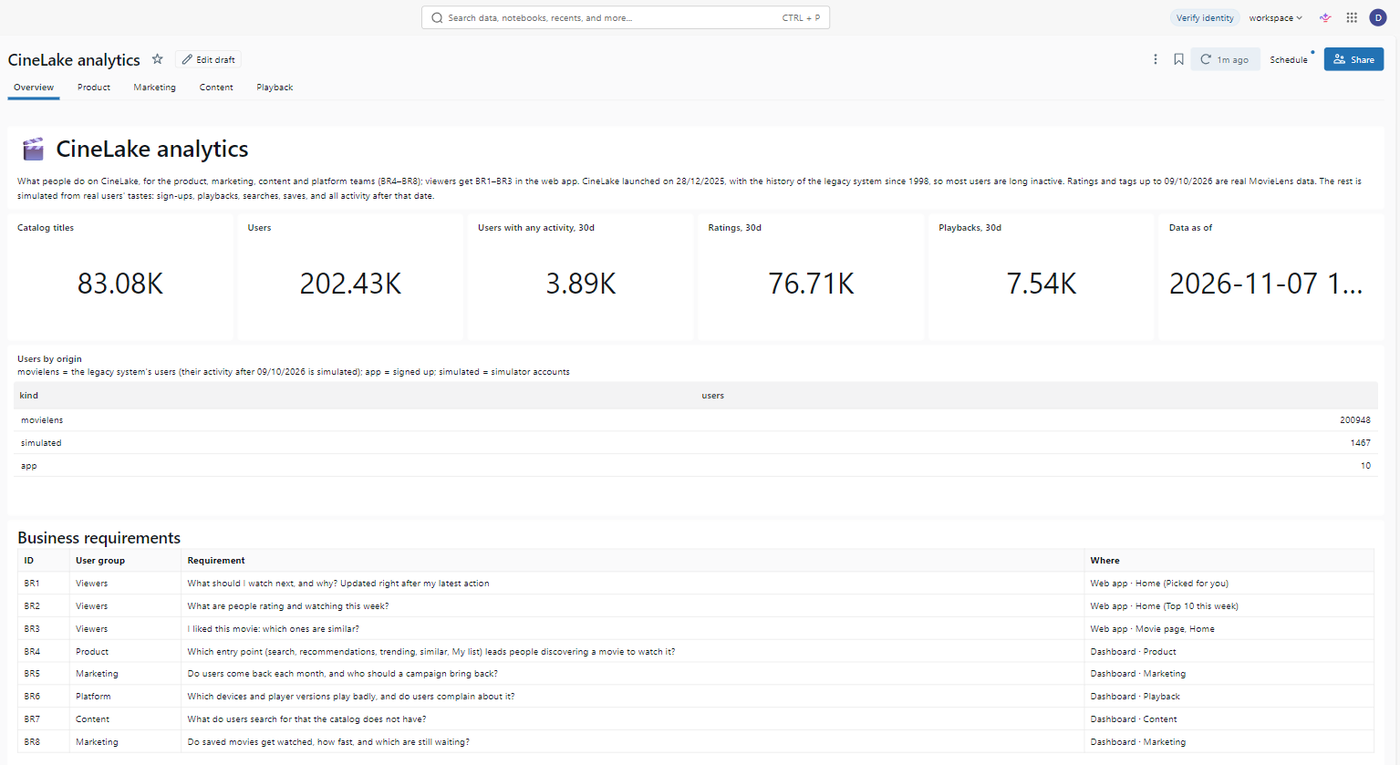
\includegraphics[width=\linewidth,height=0.84\textheight,keepaspectratio]{./images/hinh-07-overview.png}
\caption[Dashboard phân tích, trang Overview (mục 4.1)]{Dashboard phân tích, trang Overview: số liệu chung và bảng 8 BR, mỗi BR trả lời ở đâu.}
\label{fig:07}
\end{figure}

\subsection{Phân tích từng BR}\label{sec:4.2}

Phần này trình bày nhu cầu dữ liệu của từng BR, kết quả khai thác trên ứng dụng và cách đội liên quan sử dụng kết quả. Số liệu và hình ảnh được ghi nhận ngày 08/11/2026; web app được kiểm thử bằng tài khoản mới, còn dashboard được ghi nhận sau khi vòng daily kết thúc lúc 03:32.

\subsubsection*{BR1 \textperiodcentered{} Gợi ý cá nhân (Viewers, web app)}

BR1 đáp ứng nhu cầu xác định nội dung phù hợp để xem tiếp. Trong kịch bản kiểm thử, một tài khoản mới lọc thể loại Horror (Hình 9) và chấm 5 sao cho \textit{Hereditary}. Sau thao tác này, hàng \textquotedbl{}Picked for you\textquotedbl{} chuyển từ danh sách Top 10 phổ biến sang 10 phim kinh dị, giật gân, gồm \textit{Midsommar}, \textit{The Witch}, \textit{Get Out}, \textit{Us} và \textit{It Follows}. Năm phim đầu tiên hiển thị lý do \textquotedbl{}Because you liked Hereditary\textquotedbl{} (Hình 10). Gợi ý cá nhân được cập nhật ngay sau hành động đầu tiên, không phụ thuộc vào vòng cập nhật của lakehouse.

\begin{figure}[H]
\centering
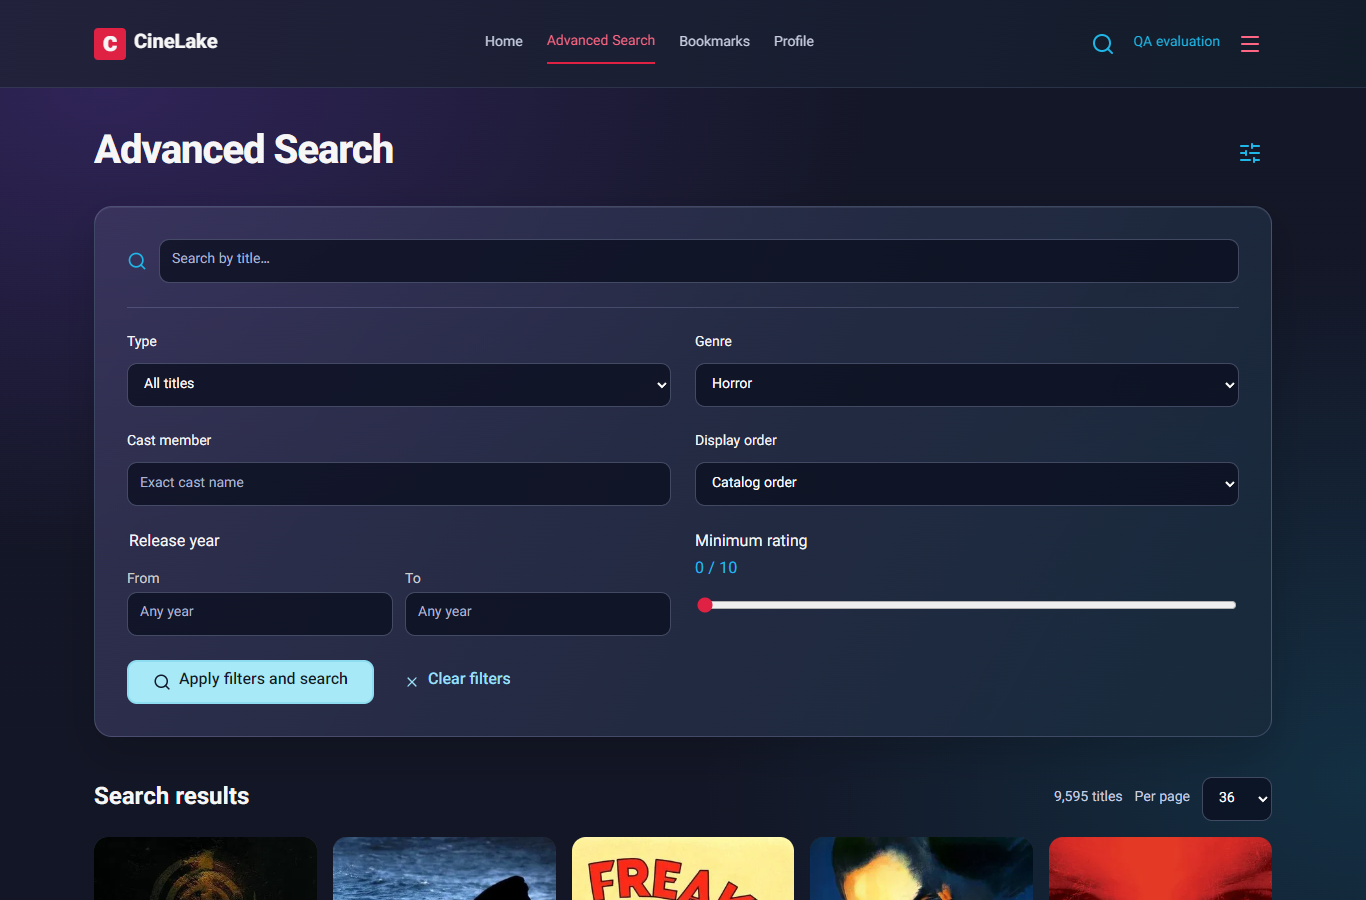
\includegraphics[width=\linewidth,height=0.84\textheight,keepaspectratio]{./images/hinh-08-br1-tim-phim-kinh-di.png}
\caption[BR1: lọc thể loại Horror trong Advanced Search (mục 4.2)]{BR1: tài khoản mới lọc thể loại Horror trong Advanced Search.}
\label{fig:08}
\end{figure}

\begin{figure}[H]
\centering
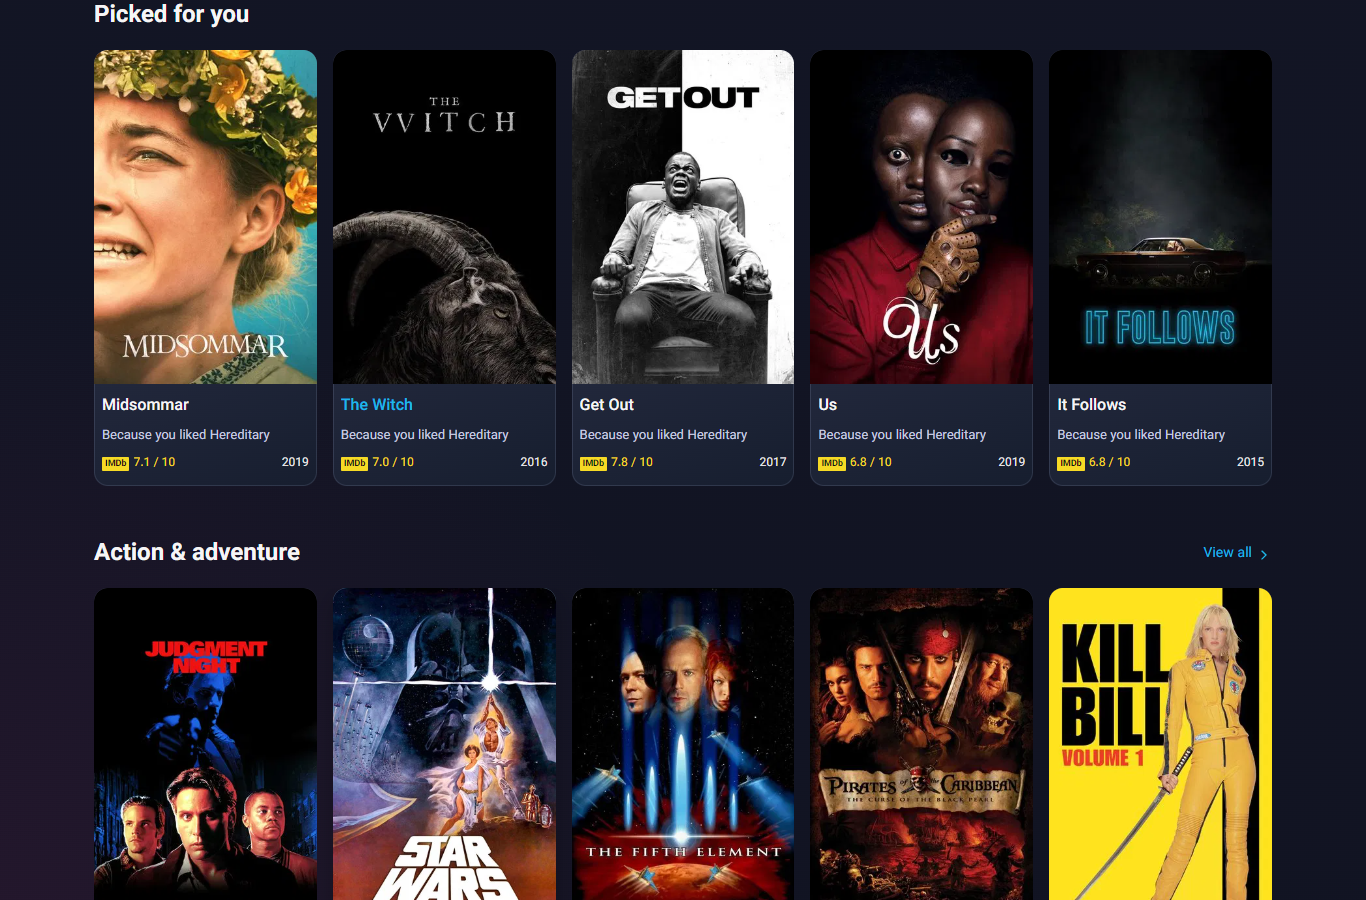
\includegraphics[width=\linewidth,height=0.84\textheight,keepaspectratio]{./images/hinh-09-br1-goi-y-ca-nhan.png}
\caption[BR1: \textquotedbl{}Picked for you\textquotedbl{} sau khi chấm 5 sao Hereditary (mục 4.2)]{BR1: \textquotedbl{}Picked for you\textquotedbl{} sau khi chấm 5 sao Hereditary.}
\label{fig:09}
\end{figure}

\subsubsection*{BR2 \textperiodcentered{} Xu hướng trong tuần (Viewers, web app)}

Đối với tài khoản chưa có lịch sử hoạt động, hàng \textquotedbl{}Top 10 this week\textquotedbl{} cung cấp danh sách khởi đầu. Tại thời điểm ghi nhận ngày 08/11, \textit{Cast Away} đứng hạng 1 với 60 người đã chấm điểm hoặc xem phim trong 7 ngày; tiếp theo là \textit{Spider-Man:} \textit{Across the Spider-Verse} (58) và \textit{Bullet Train} (57) (Hình 11). Bảng xếp hạng dựa trên số người dùng, không dựa trên số lượt rating, nên bao gồm cả người xem không chấm điểm. Sau hành động đầu tiên của người dùng, danh sách này được thay bằng gợi ý cá nhân của BR1.

\begin{figure}[H]
\centering
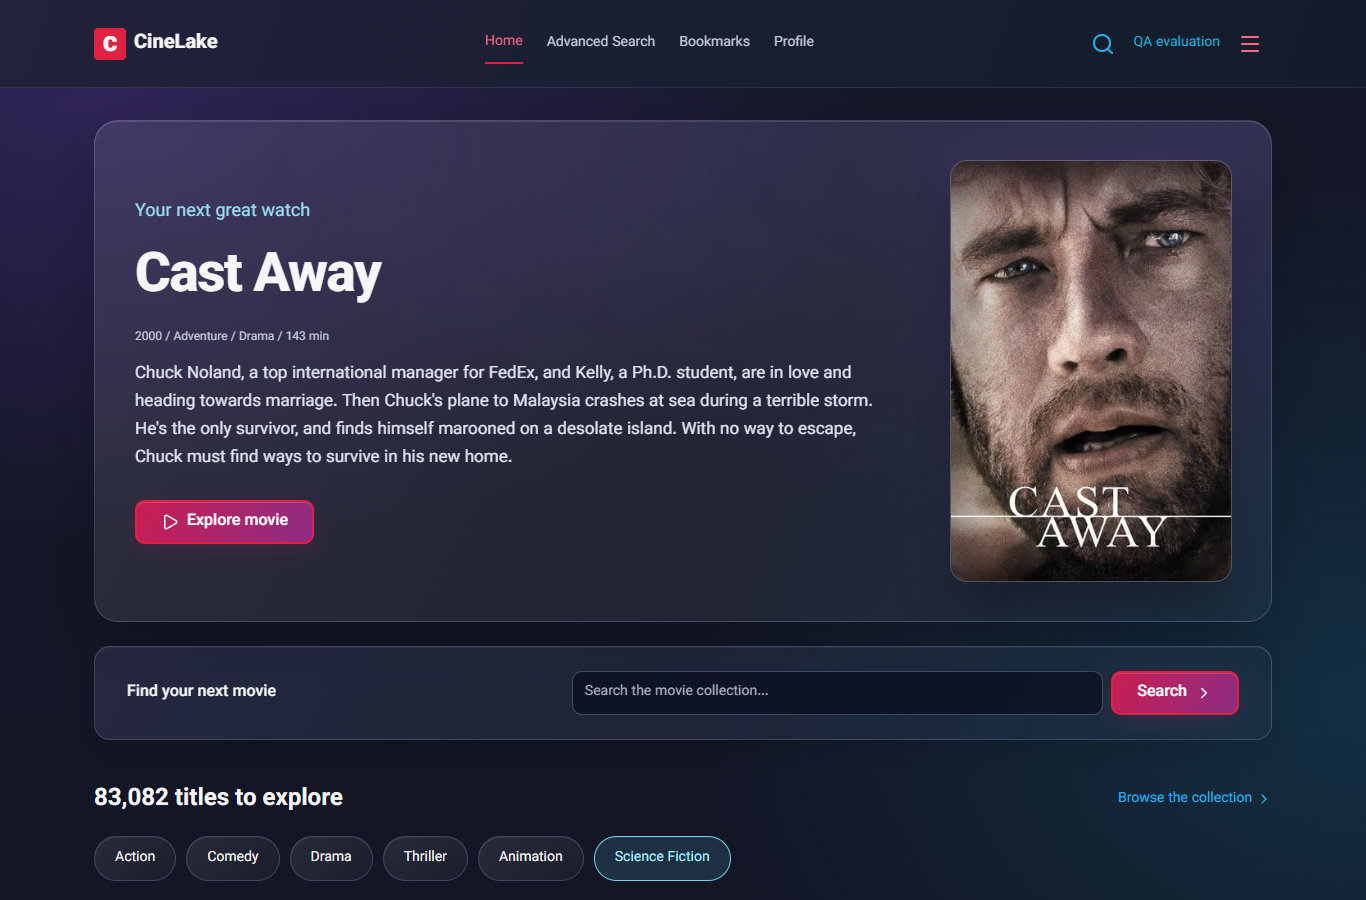
\includegraphics[width=\linewidth,height=0.84\textheight,keepaspectratio]{./images/hinh-10-br2-xu-huong.png}
\caption[BR2: trang Home và \textquotedbl{}Top 10 this week\textquotedbl{} (mục 4.2)]{BR2: trang Home của tài khoản mới; hạng 1 tuần này là Cast Away.}
\label{fig:10}
\end{figure}

\subsubsection*{BR3 \textperiodcentered{} Phim tương tự (Viewers, web app)}

BR3 giúp người xem tìm các phim có nội dung tương đồng với phim đang quan tâm. Trên trang \textit{Hereditary}, năm phim đầu tiên trong hàng \textquotedbl{}More like Hereditary\textquotedbl{} đều có ít nhất một thể loại chung; bốn phim thuộc thể loại kinh dị và \textit{Midsommar} có cùng đạo diễn Ari Aster (Hình 12). Đối với phim có ít lượt chấm điểm, hệ thống sử dụng độ tương đồng nội dung. Phương pháp này tạo được gợi ý cho 99,3\% catalog (mục 3.6).

\begin{figure}[H]
\centering
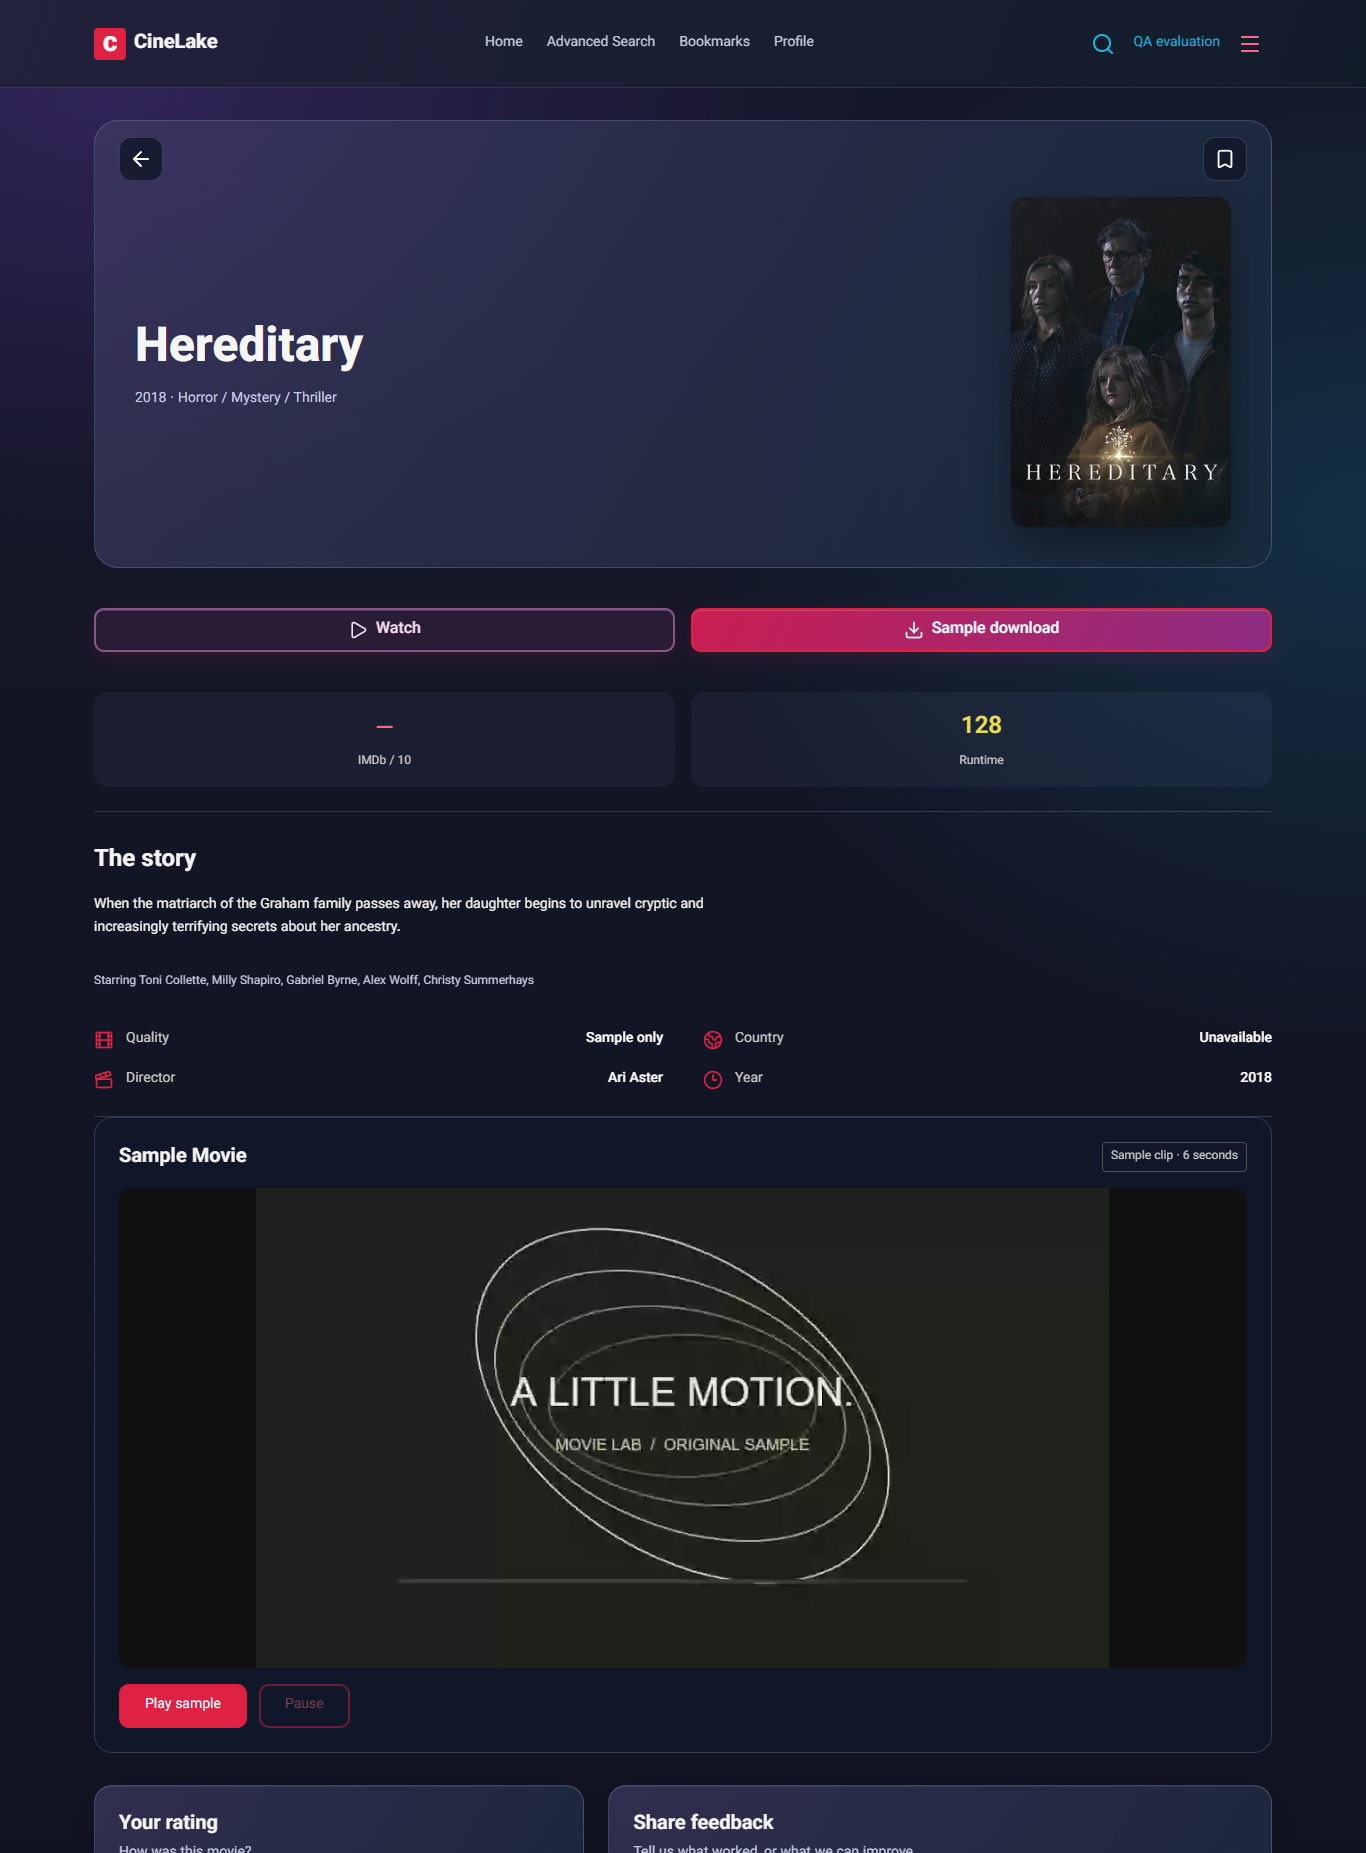
\includegraphics[width=\linewidth,height=0.88\textheight,keepaspectratio]{./images/hinh-11-br3-phim-tuong-tu-a.png}
\end{figure}
\clearpage
\begin{figure}[H]
\centering
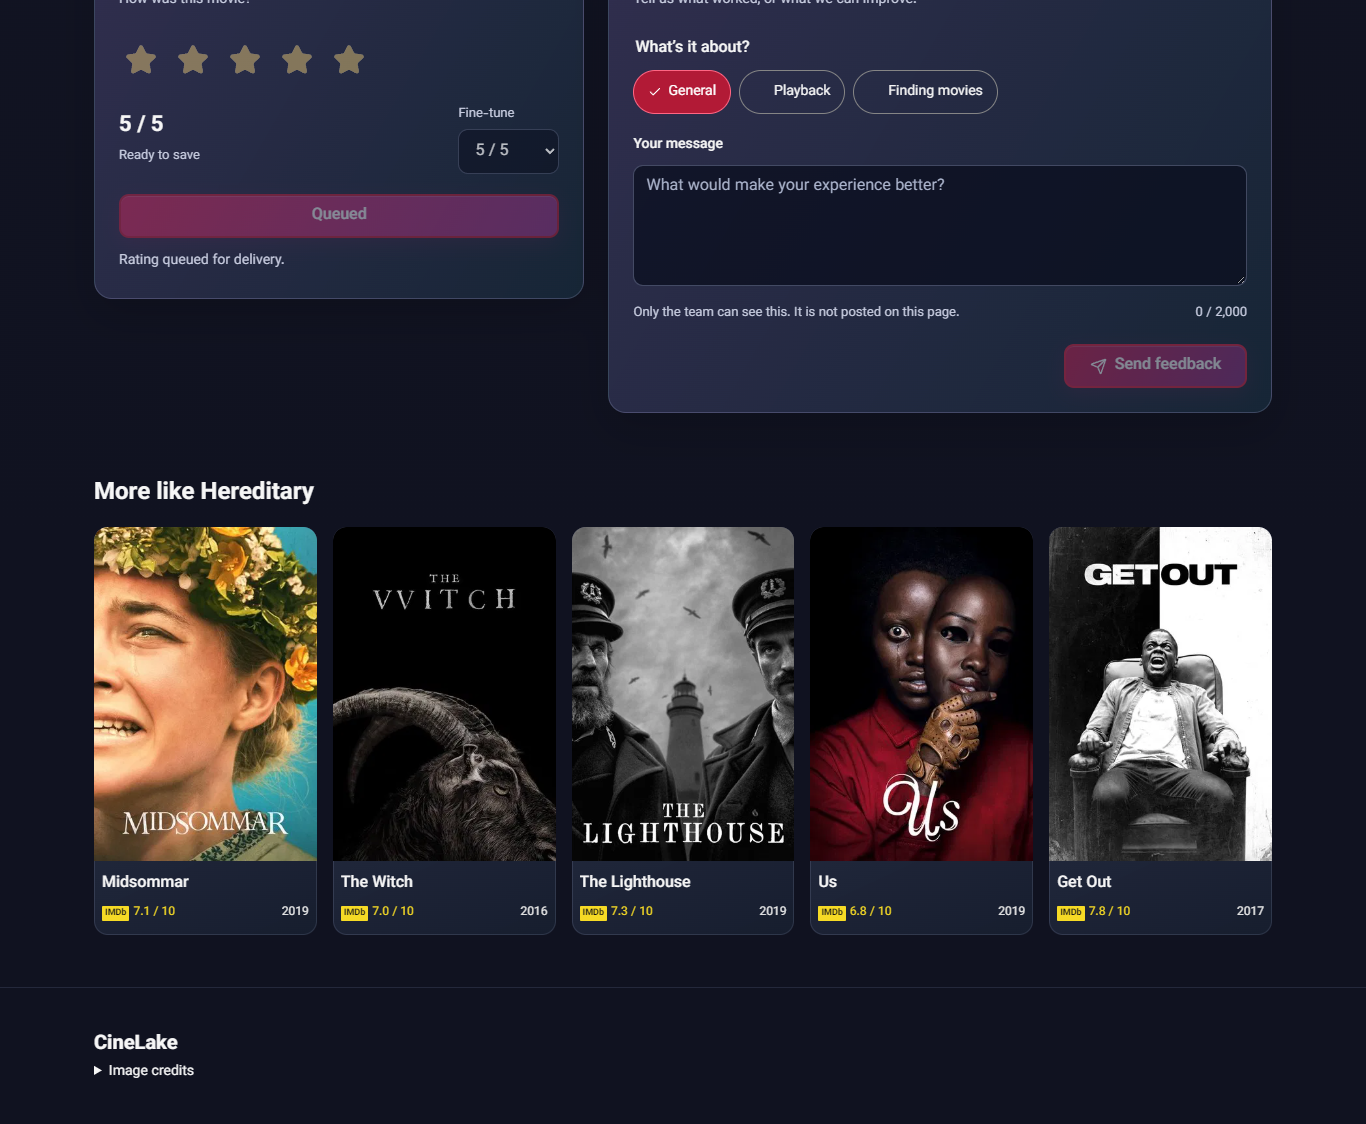
\includegraphics[width=\linewidth,height=0.84\textheight,keepaspectratio]{./images/hinh-11-br3-phim-tuong-tu-b.png}
\caption[BR3: trang phim Hereditary và \textquotedbl{}More like Hereditary\textquotedbl{} (mục 4.2)]{BR3: trang phim Hereditary và hàng \textquotedbl{}More like Hereditary\textquotedbl{}.}
\label{fig:11}
\end{figure}

\subsubsection*{BR4 \textperiodcentered{} Discovery channel dẫn tới xem phim (Product, dashboard)}

Trang dashboard của BR4 hỗ trợ đội Product xác định discovery channel nào chuyển đổi lượt khám phá phim thành lượt xem. Trong các lượt mở trang có mục đích khám phá, tìm kiếm dẫn tới xem với tỉ lệ 74,8\%, Danh sách yêu thích đạt 57,0\%, phim tương tự đạt 14,6\%, gợi ý đạt 12,5\% và trending đạt 7,1\% (Hình 13). Sau khi lượt xem bắt đầu, tỉ lệ xem hết giữa các discovery channel tương đương nhau, dao động từ 58\% đến 66\%. Kết quả cho thấy khác biệt chủ yếu nằm ở khả năng thúc đẩy người xem bắt đầu xem phim. Đội Product có thể sử dụng số liệu này để điều chỉnh thứ tự các hàng trên Home.

\begin{quote}
\textbf{Cần xét nguồn gốc dữ liệu khi diễn giải chỉ số.} Trong 75,3\% lượt mở từ gợi ý, phim tương tự và trending (839.967 lượt), mục đích là chấm điểm phim đã xem ở nơi khác, không phải khám phá nội dung. Nếu không phân loại các lượt này, hiệu quả của những channel đó sẽ bị đánh giá thấp. Pipeline gắn view intent cho từng lượt mở và chỉ đưa các lượt khám phá vào phép tính.
\end{quote}

\begin{figure}[H]
\centering
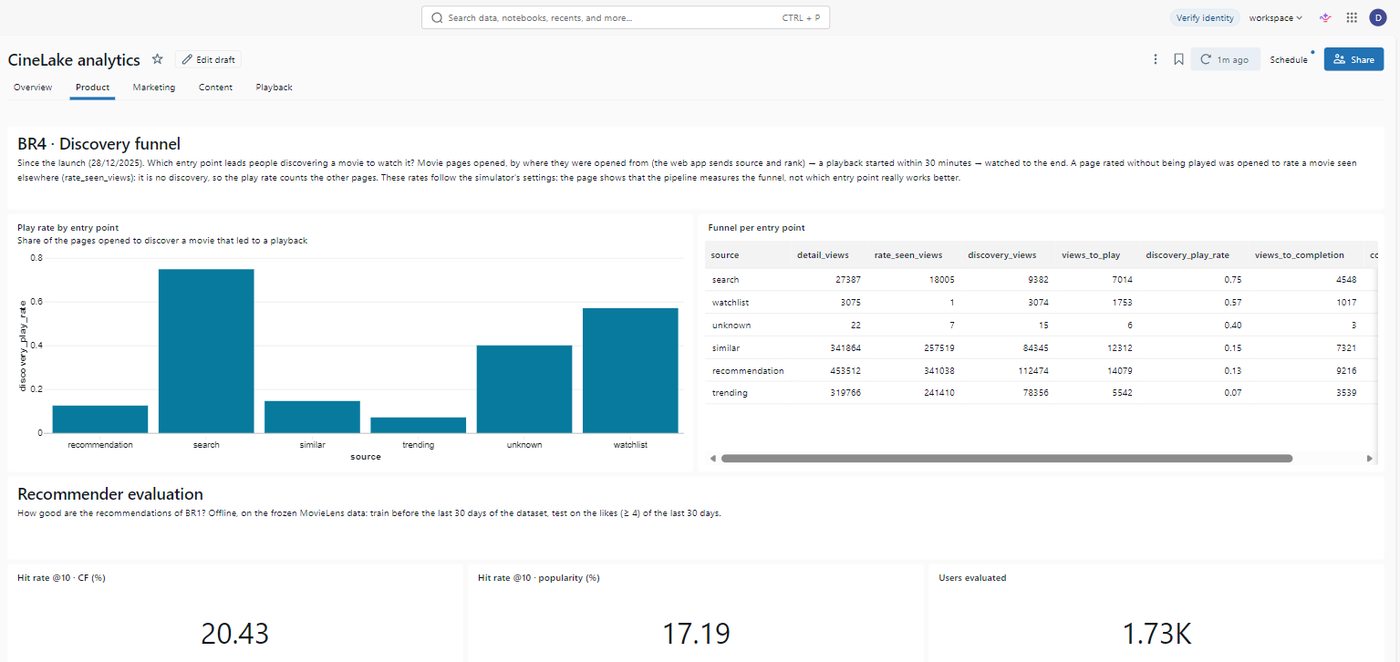
\includegraphics[width=\linewidth,height=0.84\textheight,keepaspectratio]{./images/hinh-12-br4-product.png}
\caption[BR4: dashboard, trang Product (mục 4.2)]{BR4, trang Product: tỉ lệ dẫn tới xem theo discovery channel; bên dưới là kết quả đánh giá hệ gợi ý (mục 5.3).}
\label{fig:12}
\end{figure}

\subsubsection*{BR5 \textperiodcentered{} Giữ chân user (Marketing, dashboard)}

Trang dashboard của BR5 cung cấp cho đội Marketing chỉ số giữ chân theo tháng và danh sách user cần được tiếp cận lại. Tháng 09/2026, tháng gần nhất đã chốt dữ liệu, có tỉ lệ giữ chân 64,4\% (2.048 trên 3.180 user hoạt động); tám tháng trước đó có tỉ lệ dao động từ 54,0\% đến 62,4\%. Có 3.892 user thuộc phân khúc Cooling, tức không hoạt động trong 30 ngày nhưng chưa quá 180 ngày; trong số này, 1.945 người có thể loại yêu thích là Drama (Hình 14). Danh sách kèm thể loại yêu thích có thể được tải trực tiếp từ dashboard để phục vụ chiến dịch tiếp cận lại. Khi triển khai trên nền tảng thực tế, quy trình có thể được tích hợp thêm với hệ thống email.

\begin{figure}[H]
\centering
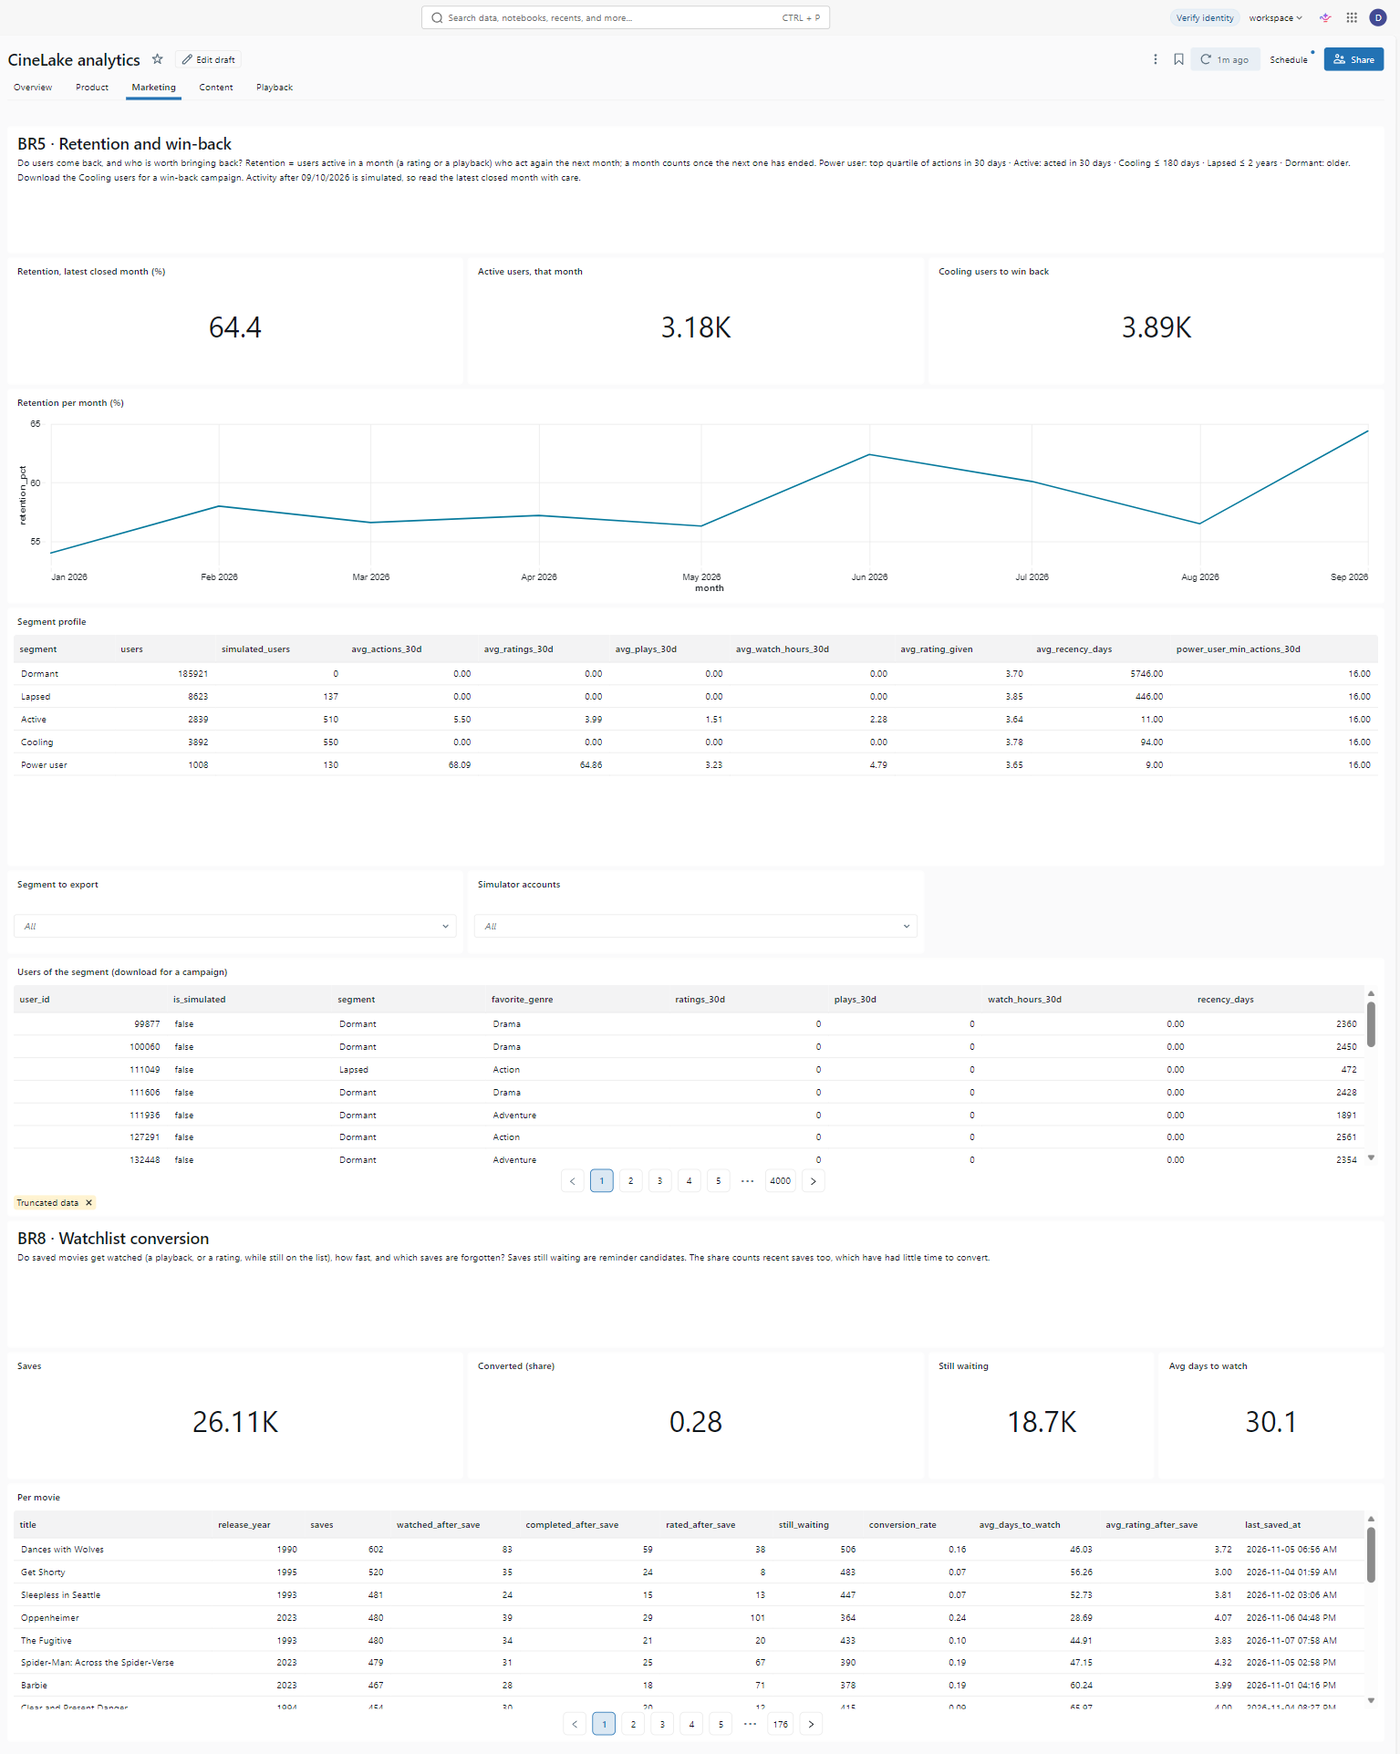
\includegraphics[width=\linewidth,height=0.84\textheight,keepaspectratio]{./images/hinh-13-br5-br8-marketing.png}
\caption[BR5 và BR8: dashboard, trang Marketing (mục 4.2)]{Trang Marketing: BR5 (giữ chân, danh sách user cần kéo lại) ở trên, BR8 (chuyển đổi từ Danh sách yêu thích) ở dưới.}
\label{fig:13}
\end{figure}

\subsubsection*{BR6 \textperiodcentered{} Chất lượng phát (Platform, dashboard)}

Trang dashboard của BR6 hỗ trợ đội phát triển Platform theo dõi chất lượng phát theo thiết bị và phiên bản player, đồng thời đối chiếu với phản hồi của người dùng. Trên mobile, phiên bản 4.0.7 có tỉ lệ lỗi 2,8\%, thời gian khởi động p95 cao nhất theo ngày là 8.933 ms và 72,7 phản hồi trên 1.000 lượt xem. Trong khi đó, phiên bản 4.1.2 trên cùng thiết bị có tỉ lệ lỗi 1,1\%, thời gian khởi động 4.227 ms và 26,9 phản hồi trên 1.000 lượt xem (Hình 15).

Nội dung phản hồi cũng cho thấy khác biệt giữa hai phiên bản: 81\% phản hồi gắn với phiên bản 4.0.7 liên quan đến lỗi phát (322/398), so với 59\% ở phiên bản 4.1.2 (461/782). Kết quả gợi ý ưu tiên yêu cầu cập nhật từ phiên bản 4.0.7 lên 4.1.2.

\begin{figure}[H]
\centering
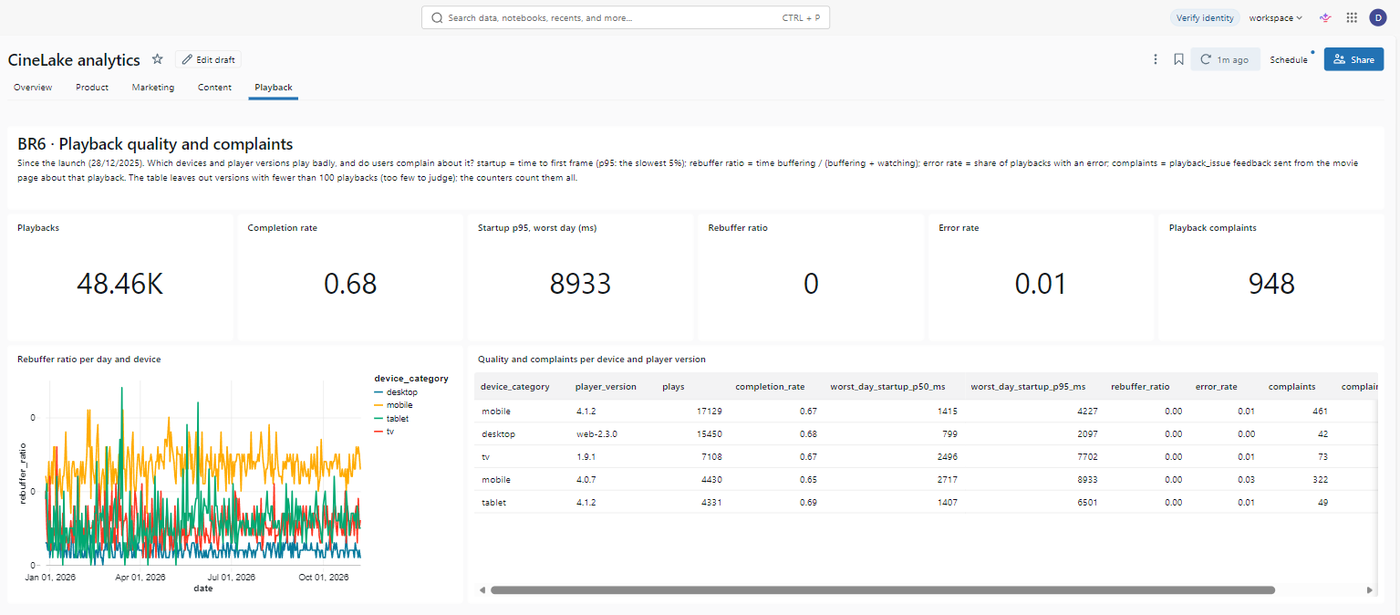
\includegraphics[width=\linewidth,height=0.84\textheight,keepaspectratio]{./images/hinh-14-br6-playback.png}
\caption[BR6: dashboard, trang Playback (mục 4.2)]{BR6, trang Playback: chất lượng phát và phàn nàn theo thiết bị và phiên bản player.}
\label{fig:14}
\end{figure}

\subsubsection*{BR7 \textperiodcentered{} Phim người dùng tìm mà catalog chưa có (Content, web app và dashboard)}

Trang dashboard của BR7 cung cấp cho đội Content thông tin về nhu cầu tìm kiếm đối với các phim chưa có trong catalog. Trong 50.233 lượt tìm kiếm bằng văn bản, 40,0\% không trả về kết quả (Hình 16).

Trong số lượt tìm kiếm không có kết quả, 57,8\% tập trung ở 125 chuỗi được lặp lại từ 5 người trở lên. Các chuỗi có tần suất cao nhất gồm tên phim phát hành sau năm 2023 (\textquotedbl{}wicked for good\textquotedbl{}: 1.252 lượt, \textquotedbl{}zootopia 2\textquotedbl{}: 730 lượt, \textquotedbl{}avatar fire and ash\textquotedbl{}: 630 lượt) và phim Việt (\textquotedbl{}mai tran thanh\textquotedbl{}: 442 lượt, \textquotedbl{}lat mat 7\textquotedbl{}: 430 lượt) (Hình 17). Danh sách này có thể được sử dụng để ưu tiên bổ sung phim vào catalog theo nhu cầu. Các chuỗi còn lại phần lớn là tên phim có sẵn nhưng bị nhập sai chính tả, cho thấy nhu cầu cải thiện khả năng xử lý lỗi chính tả của chức năng tìm kiếm.

Một chỉ số khác là tỉ lệ tìm kiếm có kết quả nhưng không có lượt nhấn. Sau ngày 09/10/2026, tỉ lệ này là 24,5\% (1.060/4.324). Tuy nhiên, các chuỗi có tần suất cao nhất là tên phim chính xác với chỉ 1--2 kết quả (\textquotedbl{}sleepless in seattle\textquotedbl{}, \textquotedbl{}the lion king\textquotedbl{}, \textquotedbl{}cast away\textquotedbl{}). Đây là hành vi tìm kiếm rồi không chọn kết quả được chủ đích mô phỏng, không phản ánh chất lượng xếp hạng tìm kiếm. Với dữ liệu thực tế, đội Product có thể sử dụng chỉ số này để phát hiện các vấn đề về thứ hạng kết quả.

\begin{figure}[H]
\centering
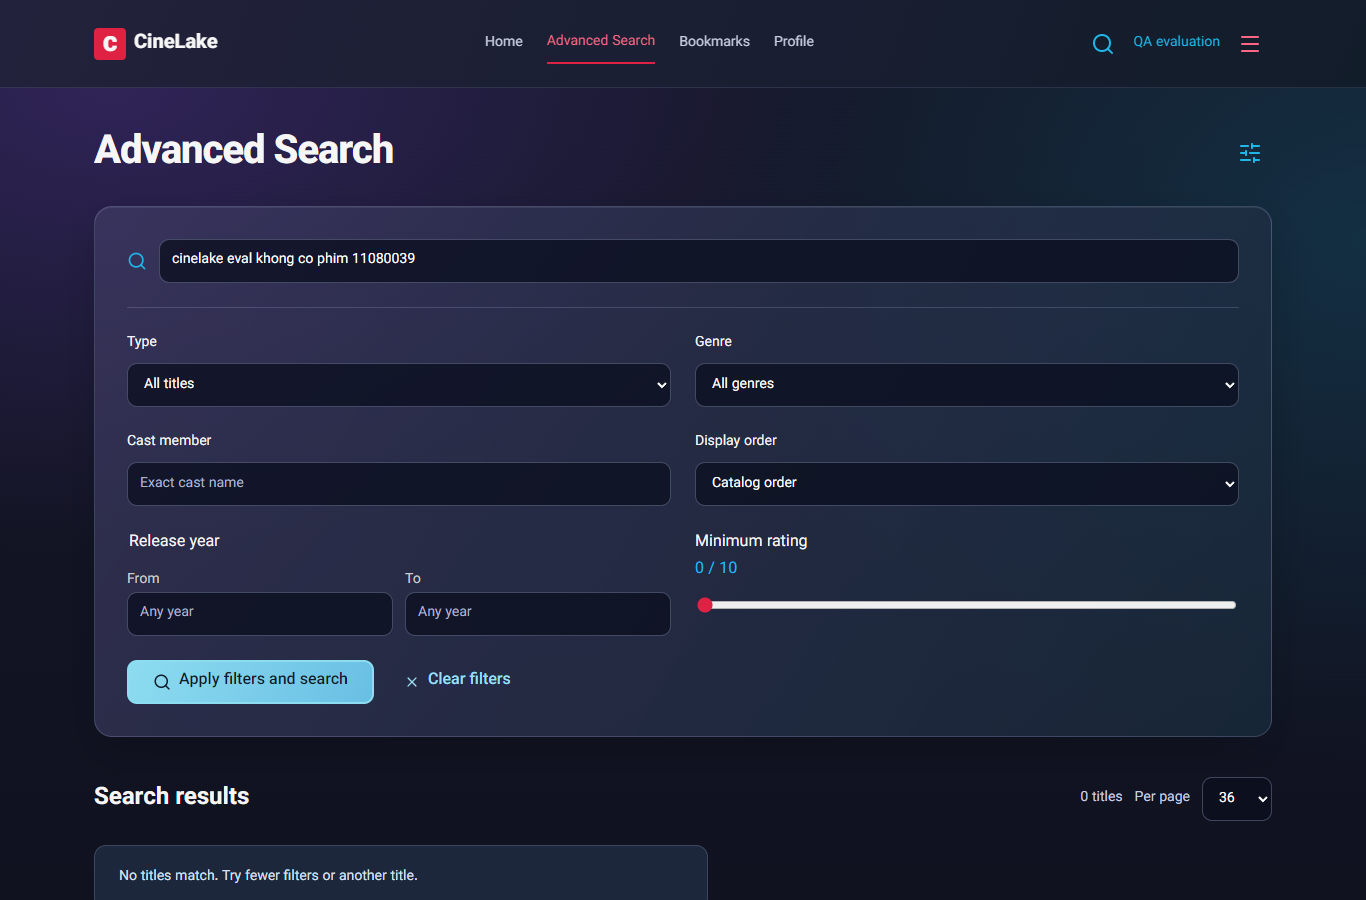
\includegraphics[width=\linewidth,height=0.84\textheight,keepaspectratio]{./images/hinh-15-br7-tim-kiem.png}
\caption[BR7 trên web: tìm phim không có trong catalog (mục 4.2)]{BR7 trên web: tìm một tên phim không có trong catalog, web trả 0 kết quả.}
\label{fig:15}
\end{figure}

\begin{figure}[H]
\centering
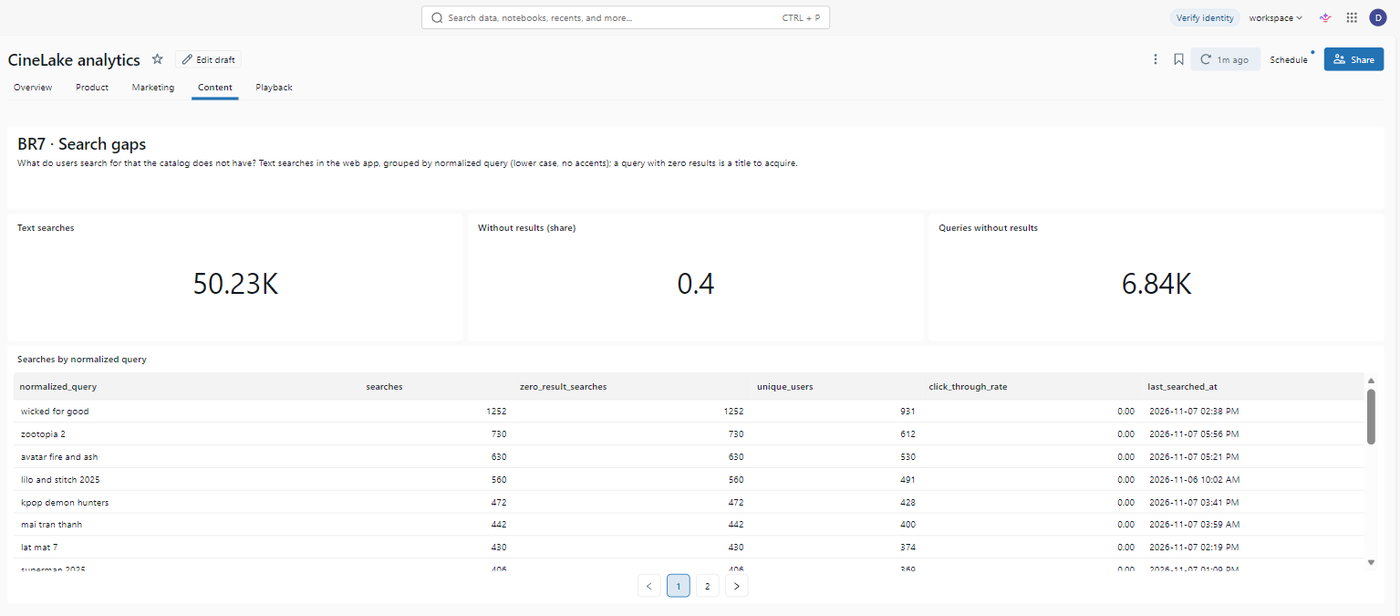
\includegraphics[width=\linewidth,height=0.84\textheight,keepaspectratio]{./images/hinh-16-br7-content.png}
\caption[BR7 trên dashboard, trang Content (mục 4.2)]{BR7 trên dashboard, trang Content: các từ khoá tìm không ra phim, xếp theo số lượt tìm.}
\label{fig:16}
\end{figure}

\subsubsection*{BR8 \textperiodcentered{} Phim đã lưu có được xem không (Marketing, dashboard)}

Trang dashboard của BR8 hỗ trợ đội Marketing theo dõi tỉ lệ chuyển đổi từ Danh sách yêu thích sang lượt xem. Trong 26.114 lần lưu, 28,4\% phim được xem hoặc chấm điểm khi vẫn còn trong danh sách; thời gian trung bình đến hành động là 30,1 ngày và trung vị là 16 ngày. Có 18.704 lần lưu vẫn đang chờ chuyển đổi (Hình 14). Danh sách phim này có thể được sử dụng làm đầu vào cho email hoặc thông báo nhắc xem. Trên web app, trang Bookmarks của tài khoản kiểm thử thể hiện hai trạng thái được Pipeline phân biệt: \textit{The} \textit{Dark Knight} chỉ được lưu, còn \textit{Pulp Fiction} được lưu rồi chấm 4 sao (Hình 18).

\begin{figure}[H]
\centering
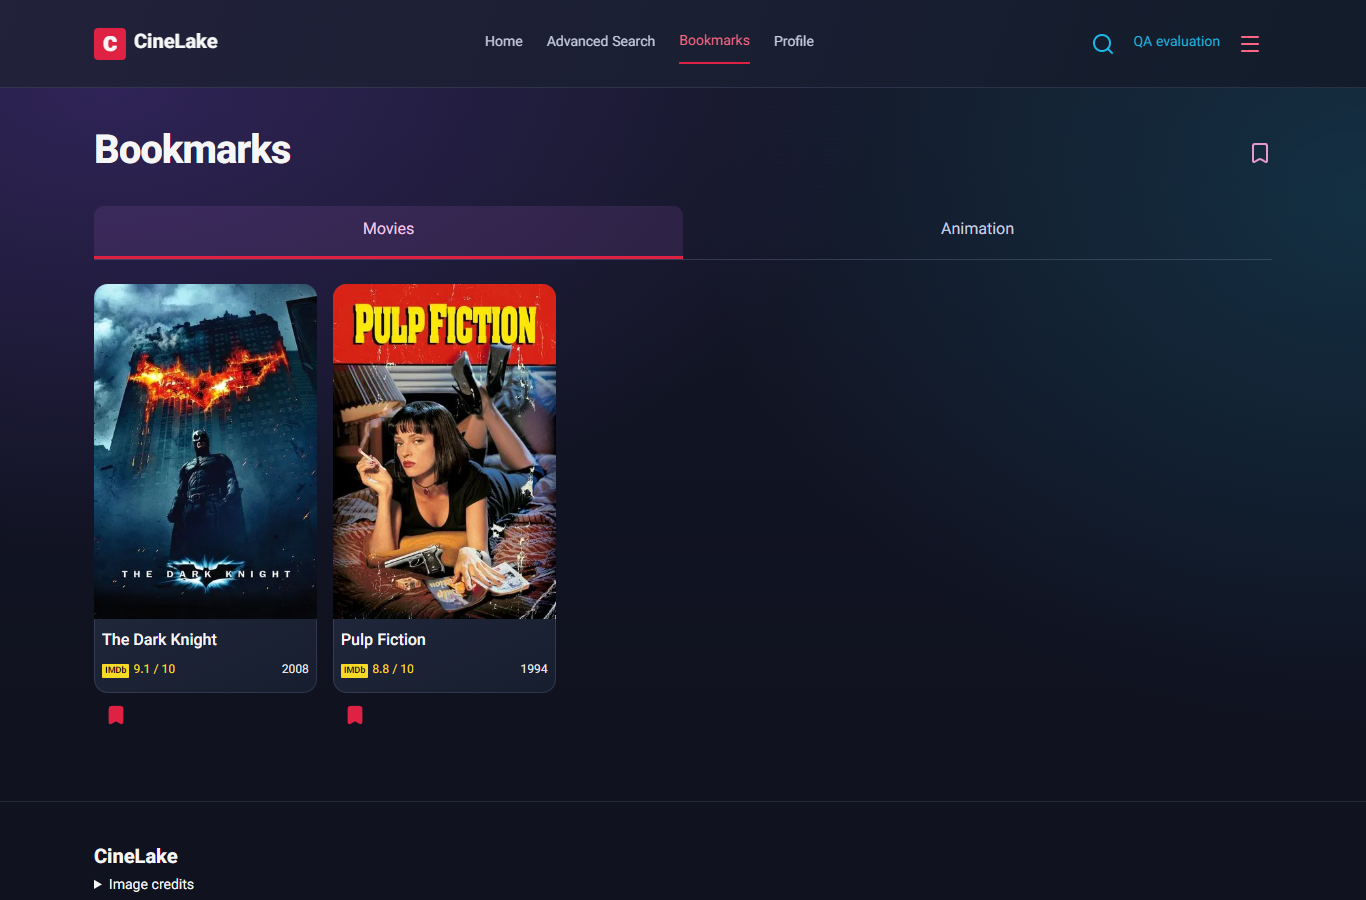
\includegraphics[width=\linewidth,height=0.84\textheight,keepaspectratio]{./images/hinh-17-br8-my-list.png}
\caption[BR8 trên web: Danh sách yêu thích (mục 4.2)]{BR8 trên web: Danh sách yêu thích (trang Bookmarks) có The Dark Knight (chỉ lưu) và Pulp Fiction (lưu rồi chấm 4 sao). Phần BR8 trên dashboard ở Hình 14.}
\label{fig:17}
\end{figure}

\section{Đánh giá}\label{sec:5}

Đề yêu cầu ba tiêu chí: độ đúng của dữ liệu (5.1), hiệu năng của giải pháp (5.2) và hiệu quả hỗ trợ khai thác dữ liệu qua ứng dụng (5.4); mục 5.3 đánh giá thêm hệ gợi ý, mục 5.5 trình bày giải pháp thay thế và đánh giá công nghệ. Mọi số liệu đo ngày 08/11/2026 (giờ Việt Nam) trên hệ thống đang chạy; số của lakehouse lấy sau vòng daily chạy từ 03:13 đến 03:32.

\subsection{Độ đúng của dữ liệu}\label{sec:5.1}

Cả 45 DQ check đạt trong vòng daily (kiểm từ 03:19 đến 03:31), không có thay đổi nào bị quarantine. Các check phủ đủ 6 chiều chất lượng của DAMA:

\begingroup
\small
\setstretch{1.12}
\setlength{\tabcolsep}{4pt}
\renewcommand{\arraystretch}{1.18}
\setlength{\reporttablewidth}{\dimexpr\linewidth-6\tabcolsep\relax}
\begin{longtable}{@{}L{0.17\reporttablewidth} L{0.24\reporttablewidth} L{0.47\reporttablewidth} L{0.12\reporttablewidth}@{}}
\caption[DQ check theo 6 chiều DAMA (mục 5.1)]{DQ check theo 6 chiều DAMA}\label{tab:16} \\
\toprule
\textbf{Chiều} & \textbf{Hỏi gì} & \textbf{Ví dụ trong CineLake} & \textbf{Số check} \\
\midrule
\endfirsthead
\toprule
\textbf{Chiều} & \textbf{Hỏi gì} & \textbf{Ví dụ trong CineLake} & \textbf{Số check} \\
\midrule
\endhead
\midrule
\endfoot
\bottomrule
\endlastfoot
Completeness & Có thiếu dữ liệu không? & Số dòng bronze bằng số dòng trong manifest & 22 \\
Validity & Giá trị có hợp lệ không? & Rating từ 0,5 đến 5, bước 0,5 & 7 \\
Consistency & Các bảng có khớp nhau không? & Mart cộng lại đúng bằng fact & 5 \\
Uniqueness & Có trùng không? & Mỗi người chỉ có một rating cho một phim & 5 \\
Integrity & Khoá có trỏ tới dòng có thật không? & Mọi rating trỏ tới một phim có trong danh mục phim & 4 \\
Accuracy & Dữ liệu có đúng với thực tế không? & Rating phát lại qua CDC khớp từng dòng với MovieLens & 2 \\
\end{longtable}
\endgroup

\begingroup
\small
\setstretch{1.12}
\setlength{\tabcolsep}{4pt}
\renewcommand{\arraystretch}{1.18}
\setlength{\reporttablewidth}{\dimexpr\linewidth-4\tabcolsep\relax}
\begin{longtable}{@{}L{0.25\reporttablewidth} L{0.39\reporttablewidth} L{0.36\reporttablewidth}@{}}
\caption[Các kiểm tra chính và kết quả (mục 5.1)]{Các kiểm tra chính và kết quả ngày 08/11/2026}\label{tab:17} \\
\toprule
\textbf{Câu hỏi} & \textbf{Kiểm tra} & \textbf{Kết quả ngày 08/11} \\
\midrule
\endfirsthead
\toprule
\textbf{Câu hỏi} & \textbf{Kiểm tra} & \textbf{Kết quả ngày 08/11} \\
\midrule
\endhead
\midrule
\endfoot
\bottomrule
\endlastfoot
File nguồn vào bronze có đủ không? & So số dòng bronze với manifest (10 bảng) & Khớp, ví dụ 32.000.204 rating, 102.643.022 dòng người tham gia phim của IMDb \\
Rating đi qua Neon, Kafka, Volume có giữ nguyên không? & So từng rating phát lại với file MovieLens gốc & 0 dòng lệch trên 789.359 dòng \\
Có rating trùng không? & Mỗi cặp user--phim chỉ có một rating & 0 trên 32.002.850 dòng \\
Gold có mất dòng so với silver không? & So số dòng fact với silver (6 bảng fact) & 0 dòng lệch ở cả 6 bảng \\
Fact có trỏ tới phim, user không tồn tại không? & Mã phim và mã user của fact có trong dimension & 0 trên 32.002.850 dòng \\
Mart cộng lại có bằng fact không? & Cộng 4 mart của BR4, BR6, BR7, BR8 rồi so với fact & Khớp cả 4 \\
Gợi ý có chứa phim đã chấm không? & Đối chiếu gợi ý với rating đã có & 0 vi phạm \\
\end{longtable}
\endgroup

Kiểm tra rating phát lại là bằng chứng mạnh nhất cho đường CDC: 789.359 rating được ghi vào PostgreSQL, đi qua WAL, Debezium, Kafka, sink, Volume, bronze rồi MERGE vào silver, và khi so từng dòng với file MovieLens gốc thì không lệch dòng nào.

\textbf{Rà soát thêm ngoài pipeline.} Ngoài các DQ check chạy trong pipeline, nhóm rà soát lại toàn bộ 21 bảng gold (số dòng, giá trị rỗng, khoá không trùng) bằng truy vấn viết riêng, không dùng code của pipeline, và tính lại tỉ lệ giữ chân của cả 9 tháng đã chốt (01-- 09/2026) từ số user quay lại và số user hoạt động. Kết quả khớp số trên dashboard, ví dụ tháng 09/2026: 2.048 / 3.180 = 64,4\%. Tháng 10 và 11 chưa chốt nên chưa có tỉ lệ.

\textbf{Unit test.} 83 unit test chạy trong container Spark trên bảng Delta thật (trong thư mục tạm), nên câu MERGE của CDC được chạy thật. Test phủ bronze, catalog, CDC, people, gold, gợi ý, data quality, simulator, dashboard và cấu trúc bundle. Lần chạy ngày 08/11: 83/83 đạt trong 39 phút 45 giây.

\begin{figure}[H]
\centering
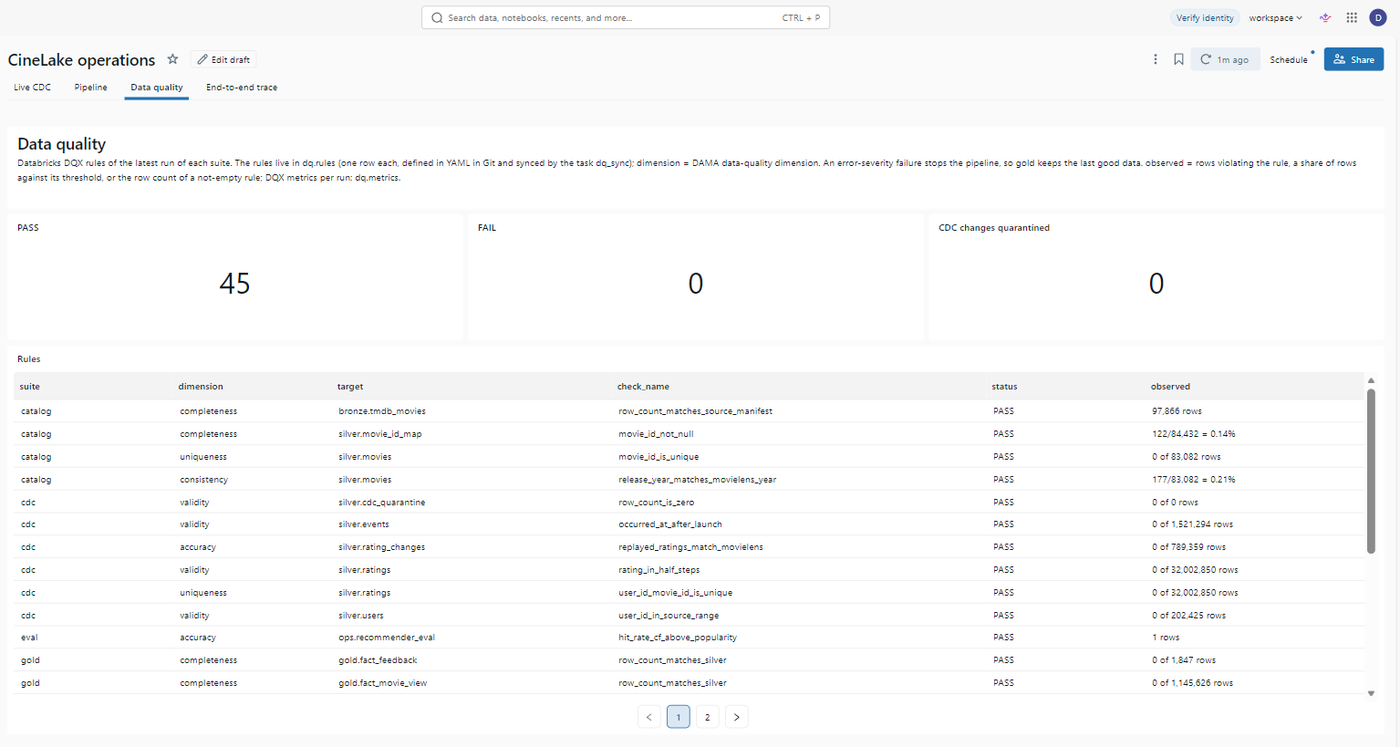
\includegraphics[width=\linewidth,height=0.84\textheight,keepaspectratio]{./images/hinh-18-data-quality.png}
\caption[Dashboard vận hành, trang Data quality (mục 5.1)]{Trang Data quality (08/11/2026): 45 DQ check PASS, 0 thay đổi bị quarantine.}
\label{fig:18}
\end{figure}

\subsection{Hiệu năng}\label{sec:5.2}

\textbf{Môi trường đánh giá.} Databricks Free Edition (compute serverless, một SQL warehouse nhỏ nhất); Neon PostgreSQL gói miễn phí; Kafka, Debezium, sink và web app trên một mini PC chạy Docker. Thời gian lấy từ nhật ký chạy của pipeline, thời điểm ghi của Kafka, lệnh EXPLAIN ANALYZE trên Neon, và trình duyệt tự động (Playwright).

\begingroup
\small
\setstretch{1.12}
\setlength{\tabcolsep}{4pt}
\renewcommand{\arraystretch}{1.18}
\setlength{\reporttablewidth}{\dimexpr\linewidth-4\tabcolsep\relax}
\begin{longtable}{@{}L{0.28\reporttablewidth} L{0.35\reporttablewidth} L{0.37\reporttablewidth}@{}}
\caption[Kết quả đánh giá hiệu năng (mục 5.2)]{Kết quả đánh giá hiệu năng ngày 08/11/2026}\label{tab:18} \\
\toprule
\textbf{Mục tiêu} & \textbf{Chi tiết đánh giá} & \textbf{Kết quả ngày 08/11/2026} \\
\midrule
\endfirsthead
\toprule
\textbf{Mục tiêu} & \textbf{Chi tiết đánh giá} & \textbf{Kết quả ngày 08/11/2026} \\
\midrule
\endhead
\midrule
\endfoot
\bottomrule
\endlastfoot
PostgreSQL \ensuremath{\rightarrow} Kafka & Từ lúc commit tới khi Kafka nhận tin (450 tin rating gần nhất) & Trung vị 0,85 giây, tối đa 1,32 giây \\
PostgreSQL \ensuremath{\rightarrow} Volume & Từ lúc commit tới khi file nằm trên Volume (giờ hoạt động gần nhất, Hình 6) & Trung vị 7 giây \\
Vòng refresh & Bronze \ensuremath{\rightarrow} silver \ensuremath{\rightarrow} gold \ensuremath{\rightarrow} Neon (vòng 00:58--01:05) & 7,6 phút, 35 bước \\
Vòng daily & Thêm nguồn ngoài, phim tương tự, đánh giá gợi ý & 19,3 phút, 66 bước \\
Web app đọc & API đọc bảng kết quả, gọi từ server & 0,24 giây; truy vấn trên Neon chỉ 0,04 ms \\
Gợi ý online & Hàm gợi ý online, đo trên Neon & 7--10 ms với user thông thường; 160--380 ms với user mô phỏng chấm khoảng 500 phim mỗi tuần \\
Web app ghi & Một sự kiện (chấm điểm, lưu phim) tới khi server xác nhận & 2,2--3,8 giây \\
Tải trang & Cả trang Home, gồm ảnh và các hàng phim & 1,4--4,9 giây \\
Dashboard & Một truy vấn trên SQL warehouse & 0,5--0,8 giây khi warehouse đang chạy; 8,7 giây cho truy vấn đầu tiên lúc warehouse khởi động \\
\end{longtable}
\endgroup

\textbf{Những điểm làm chậm quá trình xử lý dữ liệu}

\begin{itemize}
  \item \textbf{Vòng refresh tính bằng phút} chủ yếu do thời gian khởi động compute serverless cho từng job, không phải do khối lượng dữ liệu mỗi vòng.
  \item \textbf{Bước nặng nhất của vòng daily} là tính phim tương tự (193 giây, 2,38 triệu dòng), rồi đánh giá gợi ý (128 giây) và kéo TMDB (107 giây).
  \item \textbf{Web app chờ đường truyền, không chờ database.} Mỗi lượt đi về từ server tới Neon mất khoảng 0,24 giây; đọc cần một lượt, ghi một sự kiện cần 9--10 lượt nối tiếp. Giảm số lượt đi về là hướng sửa rẻ nhất (mục 6.4).
\end{itemize}

\begin{figure}[H]
\centering
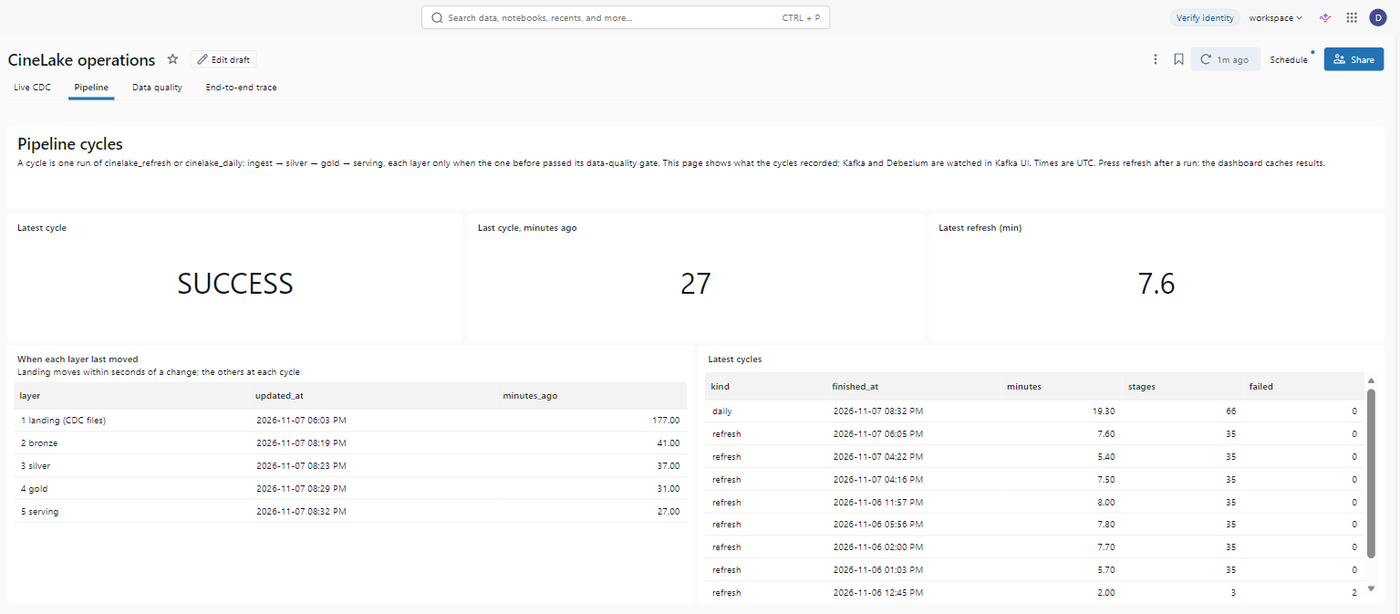
\includegraphics[width=\linewidth,height=0.84\textheight,keepaspectratio]{./images/hinh-19-pipeline.png}
\caption[Dashboard vận hành, trang Pipeline (mục 5.2)]{Trang Pipeline (08/11/2026): vòng daily 19,3 phút, vòng refresh 7,6 phút, thời điểm cập nhật của từng tầng.}
\label{fig:19}
\end{figure}

\subsection{Hệ gợi ý}\label{sec:5.3}

Gợi ý cá nhân bằng item-item CF tốt hơn gợi ý phim phổ biến trên cả ba chỉ số.

\textbf{Cách đo.} Dữ liệu MovieLens được chia theo thời gian, không chia ngẫu nhiên: học trên mọi rating trước 30 ngày cuối, kiểm tra trên 10.966 lượt thích (rating \ensuremath{\geq} 4) trong 30 ngày cuối của 1.728 user. Chia theo thời gian tránh để mô hình \textquotedbl{}nhìn trước tương lai\textquotedbl{}. Mỗi phương án gợi ý 10 phim.

\begin{itemize}
  \item \textbf{Hit rate of 10:} tỉ lệ user có ít nhất một phim trúng trong 10 gợi ý.
  \item \textbf{Precision of 10:} bao nhiêu phần gợi ý là đúng.
  \item \textbf{Recall of 10:} bao nhiêu phần phim user thật sự thích đã được gợi ý.
\end{itemize}

Kết quả vòng đánh giá ngày 08/11/2026 (Hình 21): Hit rate of 10 của CF là 20,43\% so với 17,19\% của phim phổ biến, Precision of 10 là 3,30\% so với 2,63\%, Recall of 10 là 5,21\% so với 4,15\%; tính tương đối, CF hơn 19--26\% trên cả ba chỉ số. Chênh lệch không lớn vì phim phổ biến vốn là baseline mạnh trên MovieLens, nhưng CF còn giải thích được lý do gợi ý cho từng người.

\begin{figure}[H]
\centering
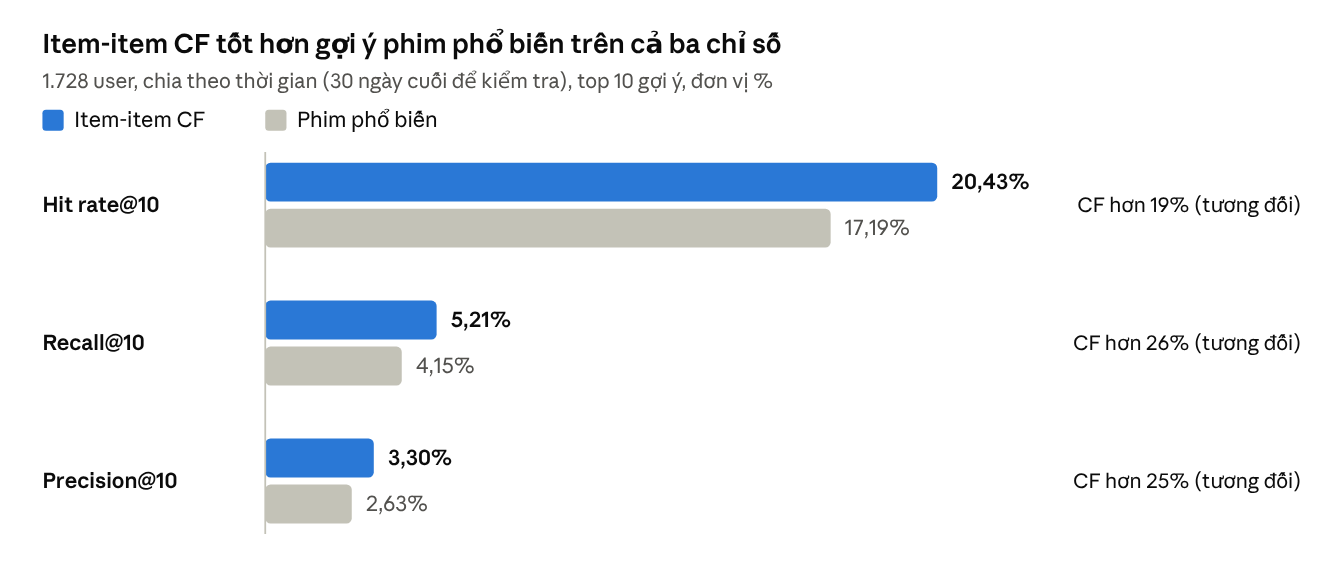
\includegraphics[width=\linewidth,height=0.84\textheight,keepaspectratio]{./images/hinh-20-danh-gia-he-goi-y.png}
{\small\itshape Đánh giá hệ gợi ý \textperiodcentered{} CF so với gợi ý phổ biến\par}
\caption[Kết quả đánh giá hệ gợi ý (mục 5.3)]{Kết quả đánh giá hệ gợi ý, vòng đánh giá ngày 08/11/2026.}
\label{fig:20}
\end{figure}

Một DQ check chặn pipeline nếu CF không còn tốt hơn phương án phổ biến, nên một thay đổi làm hỏng gợi ý sẽ không được đưa lên app. Trọng số của lớp online chưa đánh giá offline được, vì MovieLens không có lượt lưu phim, tìm kiếm hay phiên xem.

\subsection{Hiệu quả hỗ trợ khai thác dữ liệu qua ứng dụng}\label{sec:5.4}

Cả 8 BR đều được ứng dụng trả lời đúng trên hệ thống thật: trên web trong 1,4--4,9 giây, trên dashboard trong 0,5--0,8 giây khi warehouse đang chạy. Một hành động mới trên web xuất hiện trên dashboard sau một vòng cập nhật (7,6 phút).

\textbf{Cách đánh giá.} Mỗi BR thành một kịch bản có điều kiện \textquotedbl{}đạt\textquotedbl{} rõ ràng, chạy tự động ngày 08/11/2026: trình duyệt tự động (Playwright) thao tác trên web bằng một tài khoản mới; kết quả trên dashboard được kiểm bằng truy vấn trên đúng các bảng gold mà dashboard đọc. Kết quả có số và ảnh của từng BR nằm ở mục 4.2 (Hình 9--17).

\begingroup
\footnotesize
\setstretch{1.12}
\setlength{\tabcolsep}{4pt}
\renewcommand{\arraystretch}{1.18}
\setlength{\reporttablewidth}{\dimexpr\linewidth-8\tabcolsep\relax}
\begin{longtable}{@{}L{0.07\reporttablewidth} L{0.31\reporttablewidth} L{0.41\reporttablewidth} L{0.13\reporttablewidth} L{0.08\reporttablewidth}@{}}
\caption[Kịch bản kiểm thử 8 BR (mục 5.4)]{Kịch bản kiểm thử 8 BR}\label{tab:19} \\
\toprule
\textbf{BR} & \textbf{Kịch bản} & \textbf{Điều kiện đạt} & \textbf{Thời gian} & \textbf{Đạt} \\
\midrule
\endfirsthead
\toprule
\textbf{BR} & \textbf{Kịch bản} & \textbf{Điều kiện đạt} & \textbf{Thời gian} & \textbf{Đạt} \\
\midrule
\endhead
\midrule
\endfoot
\bottomrule
\endlastfoot
BR1 & Tài khoản mới lọc Horror, chấm 5 sao \textit{Hereditary}, quay về Home & \textquotedbl{}Picked for you\textquotedbl{} đổi ngay, kèm lý do & Home tải lại 4,9 giây & Đạt \\
BR2 & Mở Home & Hạng 1 của Top 10 trùng hạng 1 trong bảng do lakehouse tính & 1,4 giây & Đạt \\
BR3 & Mở trang \textit{Hereditary} & \textquotedbl{}More like\textquotedbl{} có phim cùng thể loại hoặc cùng đạo diễn & Hiện cùng trang phim & Đạt \\
BR4 & Đọc trang Product & Có tỉ lệ dẫn tới xem cho từng discovery channel, chỉ tính lượt khám phá & 0,8 giây & Đạt \\
BR5 & Đọc trang Marketing, lọc Cooling + Drama & Có tỉ lệ giữ chân tháng đã chốt và tải được danh sách & 0,7 và 0,5 giây & Đạt \\
BR6 & Đọc trang Playback & Chỉ ra phiên bản có tỉ lệ lỗi và phàn nàn cao nhất & 0,7 giây & Đạt \\
BR7 & Tìm một tên phim không có trong catalog, chờ một vòng cập nhật & Web trả 0 kết quả; từ khoá xuất hiện trên trang Content với 1 lượt tìm không ra phim & Vòng cập nhật 7,6 phút; đọc 0,6 giây & Đạt \\
BR8 & Lưu \textit{Pulp Fiction} rồi chấm 4 sao; lưu \textit{The Dark Knight} mà không chấm; chờ một vòng & Tầng gold ghi đúng \textquotedbl{}đã chấm\textquotedbl{} và \textquotedbl{}còn trong danh sách\textquotedbl{} cho từng phim & Web gửi xong 5,1 giây; vòng 7,6 phút; đọc 0,8 giây & Đạt \\
\end{longtable}
\endgroup

\begin{quote}
\textbf{Dữ liệu đi trọn một vòng.} BR7 và BR8 cho thấy một thao tác của người dùng trên web đi hết đường PostgreSQL \ensuremath{\rightarrow} Debezium \ensuremath{\rightarrow} Kafka \ensuremath{\rightarrow} Volume \ensuremath{\rightarrow} bronze \ensuremath{\rightarrow} silver \ensuremath{\rightarrow} gold rồi hiện trên dashboard của các bộ phận nội bộ. BR1 cho thấy gợi ý đổi ngay nhờ lớp online, không phải chờ vòng đó.
\end{quote}

\textbf{So với khi không có ứng dụng.} Không có dashboard, đội Marketing muốn có danh sách user Cooling thích Drama phải tự viết SQL nối rating, lượt xem, user và thể loại phim, rồi tự định nghĩa thế nào là \textquotedbl{}Cooling\textquotedbl{}. Với ứng dụng, phép tính đó đã nằm sẵn trong mart của BR5, người dùng chỉ lọc và tải về.

\textbf{Giới hạn của cách đánh giá.} Kịch bản do trình duyệt tự động thực hiện, nên chứng minh hệ thống trả đúng câu trả lời, chưa đo cảm nhận hay độ dễ dùng với người dùng mới.

\subsection{Giải pháp thay thế và đánh giá công nghệ}\label{sec:5.5}

Giải pháp thay thế là một stack mã nguồn mở tự vận hành trên server riêng. Đây là lựa chọn thực tế nhất nếu không dùng nền tảng có sẵn, và nó giữ nguyên luồng dữ liệu, nên hai phương án so được trên cùng bài toán. Phần thu thập (Debezium, Kafka) và phần phục vụ app (PostgreSQL) giữ nguyên; chỉ các thành phần Databricks được thay. Vì logic biến đổi là PySpark thuần, nó chạy được trên stack này mà không phải viết lại; riêng 65 rule chất lượng phải chuyển sang một công cụ mã nguồn mở như Great Expectations hoặc Soda Core, vì giấy phép của DQX chỉ cho dùng cùng Databricks.

\begin{figure}[H]
\centering
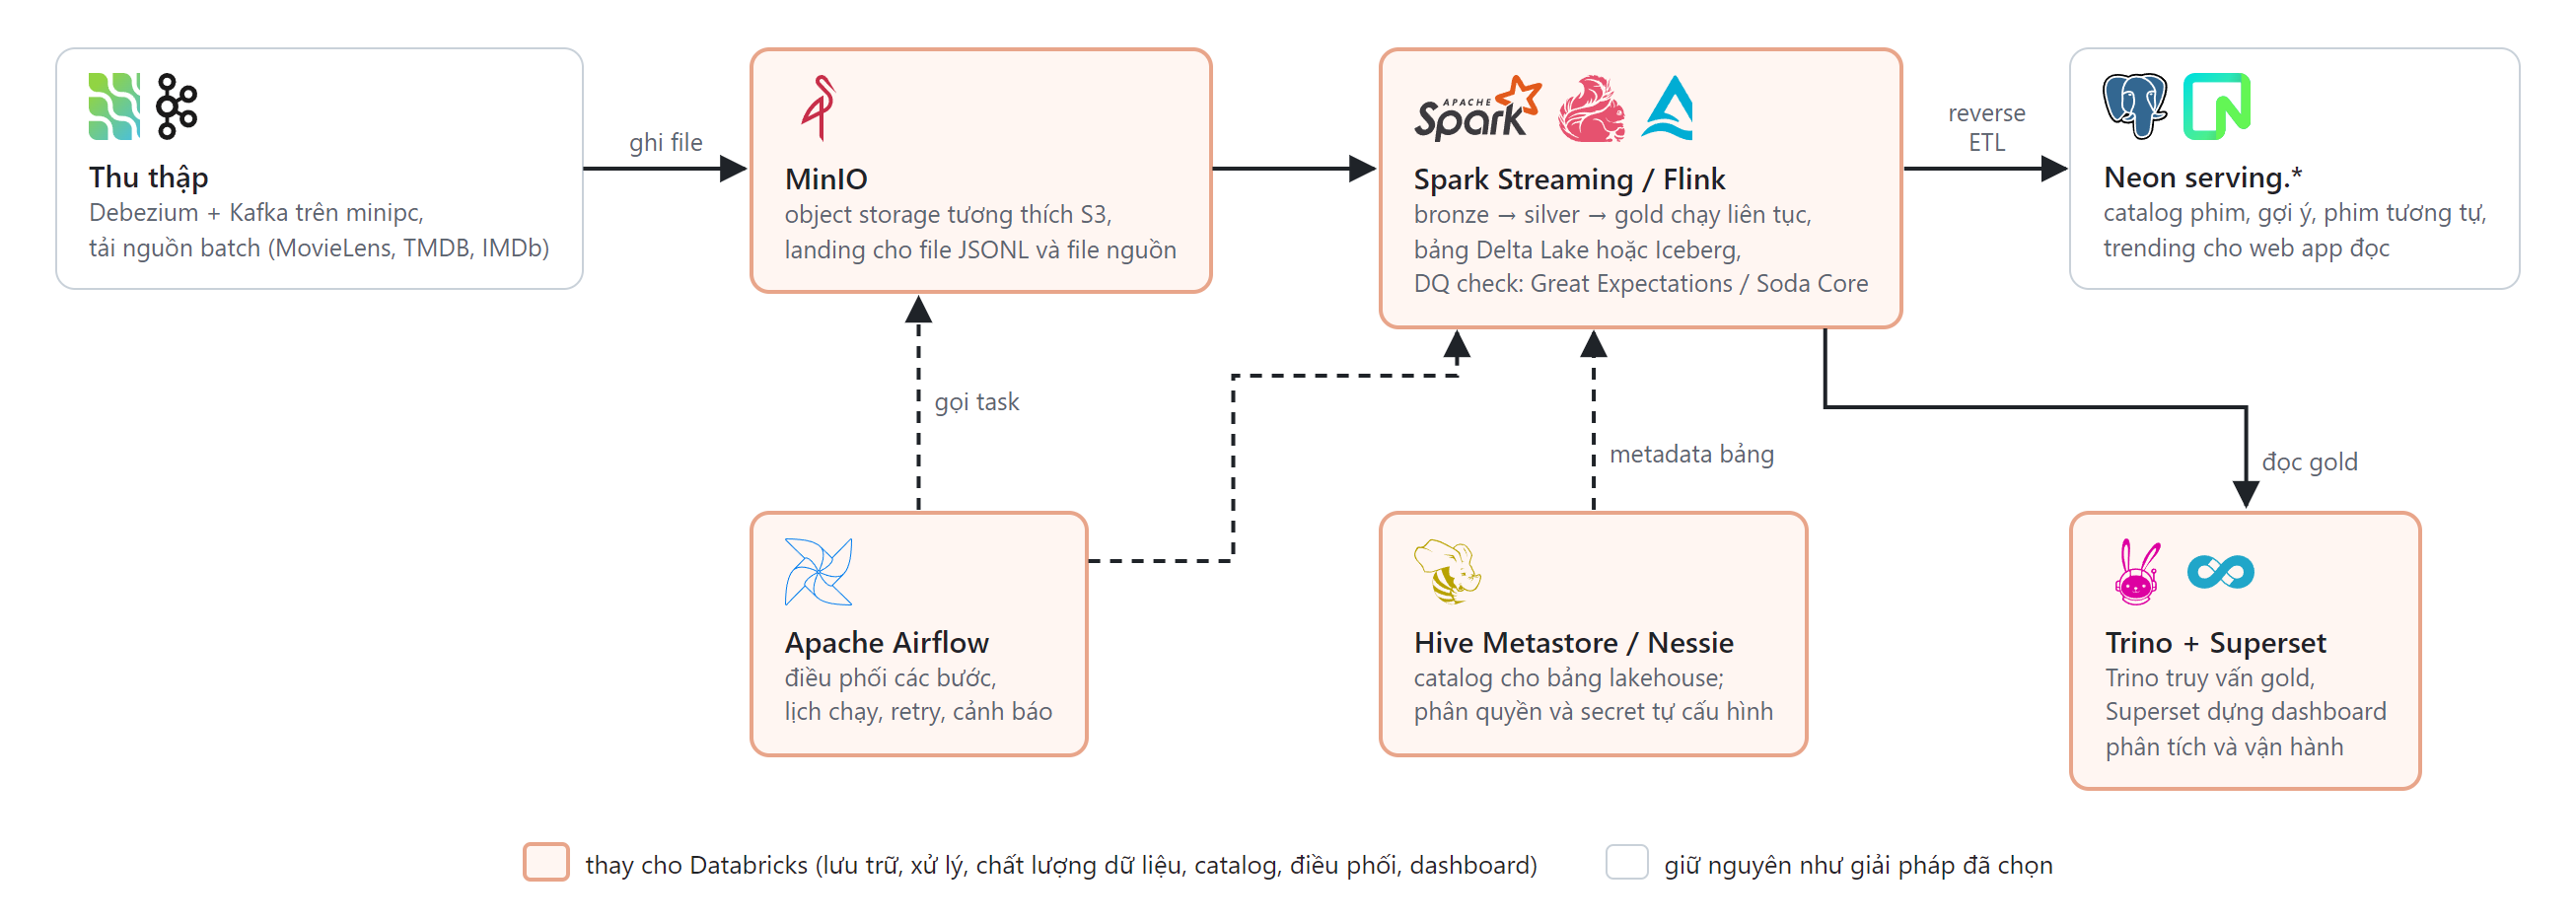
\includegraphics[width=\linewidth,height=0.84\textheight,keepaspectratio]{./images/hinh-21-kien-truc-thay-the.png}
\caption[Kiến trúc của giải pháp thay thế (mục 5.5)]{Giải pháp thay thế: stack mã nguồn mở tự vận hành; phần tô màu thay cho Databricks.}
\label{fig:21}
\end{figure}

\begingroup
\small
\setstretch{1.12}
\setlength{\tabcolsep}{4pt}
\renewcommand{\arraystretch}{1.18}
\setlength{\reporttablewidth}{\dimexpr\linewidth-4\tabcolsep\relax}
\begin{longtable}{@{}L{0.20\reporttablewidth} L{0.39\reporttablewidth} L{0.41\reporttablewidth}@{}}
\caption[Giải pháp đã chọn và giải pháp thay thế (mục 5.5)]{Giải pháp đã chọn và giải pháp thay thế}\label{tab:20} \\
\toprule
\textbf{Vai trò} & \textbf{Giải pháp đã chọn} & \textbf{Giải pháp thay thế} \\
\midrule
\endfirsthead
\toprule
\textbf{Vai trò} & \textbf{Giải pháp đã chọn} & \textbf{Giải pháp thay thế} \\
\midrule
\endhead
\midrule
\endfoot
\bottomrule
\endlastfoot
Lưu file thô & Unity Catalog Volume & MinIO (giao diện S3) \\
Định dạng bảng & Delta Lake & Delta Lake hoặc Apache Iceberg \\
Catalog, phân quyền, secret & Unity Catalog & Hive Metastore hoặc Nessie, tự cấu hình quyền \\
Xử lý & Spark trên serverless, chạy theo vòng & Spark chạy liên tục, hoặc Apache Flink \\
Chất lượng dữ liệu & DQX & Great Expectations hoặc Soda Core; phải viết lại 65 rule vì giấy phép DQX chỉ cho dùng cùng Databricks \\
Điều phối & Databricks Jobs & Apache Airflow \\
Dashboard & Databricks AI/BI & Apache Superset trên Trino \\
\end{longtable}
\endgroup

\begin{quote}
\textbf{Rủi ro hệ sinh thái.} Khi dựng thử stack này, MinIO đã ngừng phát hành Docker image cộng đồng. Nhóm thử SeaweedFS thay thế nhưng nó không tương thích với Delta, nên cuối cùng phải dùng một bản lưu trữ cũ của MinIO. Với nền tảng có sẵn, loại sự cố này do nhà cung cấp xử lý.
\end{quote}

Databricks Free Edition đáp ứng tốt 6 trên 9 tiêu chí; điểm yếu chính là quota theo ngày. Bảng dưới định nghĩa từng tiêu chí, ghi kết quả đo trên CineLake ngày 08/11/2026, và đặt cạnh stack mã nguồn mở tự vận hành ở trên và Databricks trả phí. Cột trả phí tách giới hạn của nền tảng khỏi giới hạn của gói miễn phí.

\begingroup
\footnotesize
\setstretch{1.12}
\setlength{\tabcolsep}{4pt}
\renewcommand{\arraystretch}{1.18}
\setlength{\reporttablewidth}{\dimexpr\linewidth-8\tabcolsep\relax}
\begin{longtable}{@{}L{0.16\reporttablewidth} L{0.22\reporttablewidth} L{0.23\reporttablewidth} L{0.24\reporttablewidth} L{0.15\reporttablewidth}@{}}
\caption[Đánh giá công nghệ theo 9 tiêu chí (mục 5.5)]{Đánh giá công nghệ theo 9 tiêu chí}\label{tab:21} \\
\toprule
\textbf{Tiêu chí} & \textbf{Định nghĩa và cách đo} & \textbf{Databricks Free (đo trên CineLake)} & \textbf{Stack mã nguồn mở tự vận hành} & \textbf{Databricks trả phí} \\
\midrule
\endfirsthead
\toprule
\textbf{Tiêu chí} & \textbf{Định nghĩa và cách đo} & \textbf{Databricks Free (đo trên CineLake)} & \textbf{Stack mã nguồn mở tự vận hành} & \textbf{Databricks trả phí} \\
\midrule
\endhead
\midrule
\endfoot
\bottomrule
\endlastfoot
Độ trễ & Thời gian xử lý một vòng từ landing tới khi kết quả dùng được; đo bằng thời gian vòng job & Vừa phải: vòng 7,6 phút, tự chạy khi có file mới; phần cần tươi do lớp online trong PostgreSQL đảm nhận & Giây, nhờ xử lý chạy liên tục & Giây, nhờ streaming liên tục \\
Giới hạn tài nguyên & Lượng tính toán dùng được mỗi ngày; đo bằng số vòng chạy được & Yếu: quota theo ngày giới hạn số vòng chạy mỗi ngày & Chỉ giới hạn bởi phần cứng & Theo ngân sách \\
Chi phí & Tiền phải trả để vận hành lakehouse & Tốt: 0 USD & Tiền server và công người vận hành & Trả theo mức dùng \\
Công sức vận hành & Số bước để triển khai, cập nhật, dựng lại & Tốt: triển khai job, code và dashboard bằng một lệnh; dựng môi trường mới bằng một job & Cao: tự cài đặt, nâng cấp, sao lưu, giám sát từng thành phần & Thấp \\
Độ tin cậy & Kết quả đúng khi lỗi, chạy lại hoặc dữ liệu đến trùng; đo bằng số dòng lệch và số vòng lỗi & Tốt: 0 dòng lệch trên 789.359; cả hai vòng ngày 08/11 không có bước lỗi; DQ chặn trước khi ghi ra Neon; không có SLA & Tự lo sao lưu, khôi phục và giám sát & Như bản miễn phí, thêm SLA \\
Quản trị và bảo mật & Phân quyền, secret, tổ chức dữ liệu; đo bằng phần phải tự dựng & Tốt: Unity Catalog, secret scope có sẵn; không mật khẩu nào trong code & Phải ghép thêm catalog và tự cấu hình quyền & Có sẵn \\
Mở rộng trong bối cảnh Big Data & Xử lý dữ liệu lớn mà không cấu hình hạ tầng; đo bằng khối lượng lớn nhất đã xử lý & Tốt: 233,1 triệu dòng bronze và 32 triệu rating trên serverless, không cấu hình cluster & Tự thêm node và cấu hình cluster & Tự co giãn \\
Phụ thuộc nền tảng & Phần phải viết lại nếu rời nền tảng & Trung bình: logic là PySpark và Delta thuần; Auto Loader, secret scope, dashboard AI/BI và DQX là riêng & Không & Có \\
Rủi ro hệ sinh thái & Rủi ro một thành phần ngừng hỗ trợ; đo bằng sự cố gặp thật & Tốt: không gặp sự cố phía nền tảng & Nhóm tự gánh, ví dụ sự cố MinIO (khung ở trên) & Do nhà cung cấp gánh \\
\end{longtable}
\endgroup

\textbf{Vì sao stack thay thế không có số đo hiệu năng.} Nhóm đã thử chạy stack thay thế trên laptop với cùng code pipeline. Nó cho kết quả đúng, nhưng laptop không đủ bộ nhớ để chạy hết pipeline trên toàn bộ dữ liệu. Để đo công bằng, cần tự vận hành đủ Kafka, Spark, object store và Airflow trên một server riêng đủ mạnh, nằm ngoài nguồn lực của nhóm. Vì vậy phần so sánh dừng ở mức tiêu chí, và chính nhu cầu tài nguyên này là một lý do chọn nền tảng có sẵn.

\textbf{Lựa chọn của nhóm.} Nhóm chọn Databricks Free Edition vì ba điều kiện của đồ án: không có server đủ mạnh để tự vận hành đủ stack; nhóm 4 sinh viên không có người chuyên vận hành nên cần triển khai và giám sát có sẵn; và cần quản trị, bảo mật ngay từ đầu vì có dữ liệu người dùng và thông tin đăng nhập.

\textbf{Kết luận về công nghệ.} Với một nhóm sinh viên không có server mạnh và không có người chuyên vận hành, Databricks Free Edition cho phép dựng một lakehouse đầy đủ (CDC, medallion, DQ, điều phối, dashboard) chạy trên dữ liệu thật hàng trăm triệu dòng. Điểm trừ chính là độ trễ tính bằng phút; kiến trúc của CineLake tránh nó bằng cách để phần cần tươi chạy trong PostgreSQL.

\section{Kết luận}\label{sec:6}

\subsection{Kết quả đạt được}\label{sec:6.1}

Nhóm đã xây và vận hành thật một hệ thống dữ liệu khép kín: dữ liệu từ bốn nguồn vào lakehouse, qua ba tầng và 45 DQ check, rồi quay về web app và hai dashboard. Cả 8 BR được demo thành công kèm kết quả có số, đủ để mỗi đội ra một quyết định cụ thể.

\begingroup
\small
\setstretch{1.12}
\setlength{\tabcolsep}{4pt}
\renewcommand{\arraystretch}{1.18}
\setlength{\reporttablewidth}{\dimexpr\linewidth-4\tabcolsep\relax}
\begin{longtable}{@{}L{0.25\reporttablewidth} L{0.14\reporttablewidth} L{0.61\reporttablewidth}@{}}
\caption[Kết quả theo yêu cầu nghiệp vụ (mục 6.1)]{Kết quả theo yêu cầu nghiệp vụ}\label{tab:22} \\
\toprule
\textbf{Mục tiêu} & \textbf{BR} & \textbf{Kết quả để ra quyết định (08/11/2026)} \\
\midrule
\endfirsthead
\toprule
\textbf{Mục tiêu} & \textbf{BR} & \textbf{Kết quả để ra quyết định (08/11/2026)} \\
\midrule
\endhead
\midrule
\endfoot
\bottomrule
\endlastfoot
O1 Tăng tương tác & BR1, BR2, BR3, BR4, BR8 & Gợi ý đổi ngay sau một lần chấm, hit rate 20,43\% so với 17,19\%; tìm kiếm là discovery channel dẫn tới xem nhiều nhất (74,8\%) \\
O2 Giữ chân & BR5, BR8 & Giữ được 64,4\% user tháng 09/2026; danh sách 1.945 user Cooling thích Drama và 18.704 lần lưu đang chờ để nhắc \\
O3 Đầu tư nội dung & BR7 & 40,0\% lượt tìm không ra kết quả; 125 chuỗi tìm lặp lại là danh sách phim cần mua \\
O4 Trải nghiệm xem & BR6 & Mobile 4.0.7 lỗi 2,8\% và 72,7 phàn nàn trên 1.000 lượt xem \ensuremath{\rightarrow} buộc cập nhật \\
\end{longtable}
\endgroup

\subsection{Bài học}\label{sec:6.2}

\begin{itemize}
  \item \textbf{Hiểu cách dữ liệu sinh ra quan trọng ngang cách tính.} BR4 sẽ cho kết luận sai nếu không tách lượt mở trang để chấm phim đã xem khỏi lượt khám phá.
  \item \textbf{Đo trên hệ thống thật làm lộ điểm nghẽn thật.} Khi đo, đường truyền tới Neon (0,24 giây mỗi lượt đi về) chiếm gần hết thời gian phản hồi của web app, chứ không phải truy vấn.
\end{itemize}

\subsection{Hạn chế}\label{sec:6.3}

\begin{itemize}
  \item BR4, BR6, BR7, BR8 dựa hoàn toàn trên hành vi mô phỏng, BR2 và BR5 dựa một phần, phần sau 09/10/2026 (mục 2.3).
  \item Lakehouse xử lý theo vòng micro-batch (7,6 phút mỗi vòng), nên số liệu trên dashboard không real-time; quota Free Edition giới hạn số vòng chạy mỗi ngày.
  \item Neon miễn phí giới hạn 100 CU-giờ mỗi tháng; Debezium giữ compute bật liên tục nên chỉ đủ khoảng 17 ngày.
  \item Web app chờ đường truyền tới Neon: đọc mất 0,24 giây, ghi một sự kiện mất 2,2--3,8 giây vì nhiều truy vấn nối tiếp.
  \item Trọng số lớp online là heuristic, chưa được học từ dữ liệu; với user hoạt động rất dày, hàm mất 160--380 ms.
  \item Chưa có cảnh báo tự động cho Debezium và sink; Databricks chỉ gửi email khi job lỗi.
  \item Chưa kiểm thử với người dùng thật, và giải pháp thay thế chưa có số đo hiệu năng.
\end{itemize}

\subsection{Hướng phát triển}\label{sec:6.4}

\begin{itemize}
  \item \textbf{Tầng nearline:} một consumer đọc thẳng Kafka (ví dụ bằng Flink) để cập nhật trending theo giờ, thay vì chờ vòng lakehouse.
  \item \textbf{Gợi ý:} thử ALS hoặc embedding; học trọng số lớp online từ dữ liệu thật; giới hạn số tín hiệu đọc mỗi user để hàm online luôn dưới 10 ms.
  \item \textbf{Backend:} gộp các bước ghi sự kiện vào một hàm SQL để còn một lượt đi về; đặt server gần vùng của Neon để giảm 0,24 giây mỗi lượt.
  \item \textbf{Quy mô lớn:} sink gom file theo khoảng 1--5 phút, và app gửi sự kiện thẳng vào Kafka thay vì ghi qua PostgreSQL.
  \item \textbf{Định dạng mở:} thử Apache Iceberg để giảm phụ thuộc nền tảng.
  \item \textbf{Giám sát:} cảnh báo khi Debezium dừng hoặc sink không ghi file trong một khoảng thời gian.
\end{itemize}

\section*{Phụ lục}
\addcontentsline{toc}{section}{Phụ lục}

\subsection*{Phụ lục A. Phân công công việc}
\addcontentsline{toc}{subsection}{A. Phân công công việc}

\begingroup
\small
\setstretch{1.12}
\setlength{\tabcolsep}{4pt}
\renewcommand{\arraystretch}{1.18}
\setlength{\reporttablewidth}{\dimexpr\linewidth-6\tabcolsep\relax}
\begin{longtable}{@{}L{0.23\reporttablewidth} L{0.43\reporttablewidth} L{0.20\reporttablewidth} L{0.14\reporttablewidth}@{}}
\caption[Phân công công việc (Phụ lục A)]{Phân công công việc}\label{tab:23} \\
\toprule
\textbf{Thành viên (MSSV)} & \textbf{Phần kỹ thuật} & \textbf{Phần trình bày} & \textbf{Mức đóng góp} \\
\midrule
\endfirsthead
\toprule
\textbf{Thành viên (MSSV)} & \textbf{Phần kỹ thuật} & \textbf{Phần trình bày} & \textbf{Mức đóng góp} \\
\midrule
\endhead
\midrule
\endfoot
\bottomrule
\endlastfoot
Nguyễn Đình Tuấn (2670389) & Bronze, silver, kiểm soát chất lượng dữ liệu; đo và tổng hợp số liệu đánh giá; tìm hiểu giải pháp thay thế & Mục 3.4, 3.5 và mục 5 & 100\% \\
Lê Tuấn Hưng (2670289) & Thu thập dữ liệu: MovieLens, TMDB, IMDb; Debezium, Kafka, sink, simulator; vận hành server & Mục 3.3; BR6, BR7 & 100\% \\
Trần Anh Khoa (2670309) & Tầng gold, hệ gợi ý, serving, dashboard & BR4, BR5, BR8 & 100\% \\
Nguyễn Tấn Dũng (2670272) & Xây dựng Web app;  thiết kế và deploy app database & BR1, BR2, BR3 & 100\% \\
\end{longtable}
\endgroup

\subsection*{Phụ lục B. Truy cập và kiểm tra sản phẩm}
\addcontentsline{toc}{subsection}{B. Truy cập và kiểm tra sản phẩm}

\begingroup
\small
\setstretch{1.12}
\setlength{\tabcolsep}{4pt}
\renewcommand{\arraystretch}{1.18}
\setlength{\reporttablewidth}{\dimexpr\linewidth-2\tabcolsep\relax}
\begin{longtable}{@{}L{0.35\reporttablewidth} L{0.65\reporttablewidth}@{}}
\caption[Địa chỉ truy cập sản phẩm (Phụ lục B)]{Địa chỉ truy cập sản phẩm}\label{tab:24} \\
\toprule
\textbf{Thành phần} & \textbf{Địa chỉ} \\
\midrule
\endfirsthead
\toprule
\textbf{Thành phần} & \textbf{Địa chỉ} \\
\midrule
\endhead
\midrule
\endfoot
\bottomrule
\endlastfoot
Web app & \url{https://cinelake.hunglechpro.id.vn} \\
Dashboard CineLake analytics & \href{https://dbc-13f9afb0-c92a.cloud.databricks.com/dashboardsv3/01f1d877b4ec15d7afa5ef27a6e02488/published?w=7474654576685354}{Mở dashboard} \\
Dashboard CineLake operations & \href{https://dbc-13f9afb0-c92a.cloud.databricks.com/dashboardsv3/01f1d95897841fa0bbcda3781d1a6aad/published?w=7474654576685354}{Mở dashboard} \\
Mã nguồn & Repo \texttt{movie-lakehouse} (pipeline, CDC, simulator, dashboard) và repo web app riêng \\
\end{longtable}
\endgroup

\textbf{Kiểm tra một vòng dữ liệu trọn vẹn:}

\begin{enumerate}
  \item Tạo tài khoản trên web app, chấm 5 sao một phim: hàng \textquotedbl{}Picked for you\textquotedbl{} ở Home đổi ngay (BR1).
  \item Mở dashboard operations, trang Live CDC: thay đổi vừa làm xuất hiện sau vài giây (trung vị 7 giây ngày 08/11/2026).
  \item Đợi một vòng xử lý lakehouse (khoảng 8 phút).
  \item Mở trang End-to-end trace: thay đổi đã đi qua bronze và silver; trang Data quality hiện 45/45 PASS.
  \item Bấm refresh trên dashboard analytics: số liệu BR4--BR8 đã gồm hành động mới.
\end{enumerate}

\subsection*{Phụ lục C. Từ viết tắt và thuật ngữ}
\addcontentsline{toc}{subsection}{C. Từ viết tắt và thuật ngữ}

\begingroup
\small
\setstretch{1.12}
\setlength{\tabcolsep}{4pt}
\renewcommand{\arraystretch}{1.18}
\setlength{\reporttablewidth}{\dimexpr\linewidth-2\tabcolsep\relax}
\begin{longtable}{@{}L{0.29\reporttablewidth} L{0.71\reporttablewidth}@{}}
\caption[Từ viết tắt và thuật ngữ (Phụ lục C)]{Từ viết tắt và thuật ngữ}\label{tab:25} \\
\toprule
\textbf{Từ} & \textbf{Nghĩa} \\
\midrule
\endfirsthead
\toprule
\textbf{Từ} & \textbf{Nghĩa} \\
\midrule
\endhead
\midrule
\endfoot
\bottomrule
\endlastfoot
BR & Business requirement, yêu cầu nghiệp vụ \\
CDC & Change Data Capture, ghi lại mọi thay đổi của database để hệ thống khác đọc \\
WAL & Write-Ahead Log, nhật ký PostgreSQL ghi mọi thay đổi trước khi lưu \\
LSN & Log Sequence Number, vị trí của một thay đổi trong WAL, chỉ tăng dần \\
CF & Collaborative filtering, gợi ý dựa trên những người có cùng sở thích \\
DQ & Data quality, chất lượng dữ liệu \\
DAMA & Hiệp hội quản lý dữ liệu quốc tế; ở đây là 6 chiều chất lượng của họ \\
Medallion & Kiến trúc ba tầng bronze, silver, gold \\
Reverse ETL & Chép kết quả từ kho phân tích về database của ứng dụng \\
Idempotent & Chạy lại nhiều lần vẫn ra cùng kết quả \\
Write-audit-publish & Ghi, kiểm tra, rồi mới công bố dữ liệu \\
Accumulating snapshot & Bảng fact mỗi dòng là một quá trình, được cập nhật dần khi các mốc xảy ra \\
Hit rate of 10 & Tỉ lệ user có ít nhất một phim trúng trong 10 gợi ý \\
Quarantine & Tách dòng dữ liệu sai sang một bảng riêng, dòng đúng đi tiếp \\
Record linkage & Ghép các bản ghi của cùng một đối tượng (ở đây là một phim) từ nhiều nguồn khác nhau \\
Mart & Bảng tổng hợp sẵn cho một câu hỏi hoặc một nhóm người dùng, đọc từ các bảng fact \\
Discovery channel & Nơi người xem bấm vào để mở trang phim: tìm kiếm, gợi ý, trending, phim tương tự, Danh sách yêu thích \\
Offline / online layer & Lớp gợi ý tính trước theo vòng trên lakehouse / lớp tính ngay lúc app hỏi trong PostgreSQL \\
Manifest & Bản ghi số dòng của từng file nguồn, dùng để kiểm tra dữ liệu có bị thiếu khi nạp không \\
View intent & Mục đích của một lượt mở trang phim: để khám phá hay chỉ để chấm phim đã xem \\
\end{longtable}
\endgroup

\subsection*{Phụ lục D. Tài liệu tham khảo}
\addcontentsline{toc}{subsection}{D. Tài liệu tham khảo}

\begin{enumerate}
  \item F. Maxwell Harper, Joseph A. Konstan. The MovieLens Datasets: History and Context. ACM Transactions on Interactive Intelligent Systems, 2015. Bộ dữ liệu MovieLens 32M: \url{https://grouplens.org/datasets/movielens/}
  \item The Movie Database (TMDB) API: \url{https://developer.themoviedb.org/}
  \item IMDb Non-Commercial Datasets: \url{https://developer.imdb.com/non-commercial-datasets/}
  \item Debezium Connector for PostgreSQL: \url{https://debezium.io/documentation/}
  \item Apache Kafka: \url{https://kafka.apache.org/documentation/}
  \item Delta Lake: \url{https://docs.delta.io/}
  \item Databricks Labs DQX: \url{https://databrickslabs.github.io/dqx/}
  \item Databricks, File arrival triggers: \url{https://docs.databricks.com/aws/en/jobs/file-arrival-triggers}
  \item DAMA International. DAMA-DMBOK: Data Management Body of Knowledge, 2nd ed., 2017.
  \item Xavier Amatriain, Justin Basilico. System Architectures for Personalization and Recommendation. Netflix Technology Blog, 2013.
  \item Michael Armbrust, Ali Ghodsi, Reynold Xin, Matei Zaharia. Lakehouse: A New Generation of Open Platforms that Unify Data Warehousing and Advanced Analytics. CIDR, 2021.
  \item Ralph Kimball, Margy Ross. The Data Warehouse Toolkit, 3rd ed. Wiley, 2013.
  \item Apache Spark, Structured Streaming Programming Guide: \url{https://spark.apache.org/docs/latest/streaming/}
  \item Databricks, Unity Catalog: \url{https://docs.databricks.com/aws/en/data-governance/unity-catalog/}
  \item Databricks, Asset Bundles: \url{https://docs.databricks.com/aws/en/dev-tools/bundles/}
  \item Neon Serverless Postgres: \url{https://neon.com/docs/}
\end{enumerate}

\subsection*{Phụ lục E. Thiết kế dữ liệu chi tiết}
\addcontentsline{toc}{subsection}{E. Thiết kế dữ liệu chi tiết}

Phụ lục này liệt kê các bảng của ba tầng bronze, silver, gold, các bảng serving mà web app đọc, và các bảng vận hành, chất lượng dữ liệu. Database của app trên Neon, nguồn của đường CDC, đã được mô tả ở mục 3.3 (Bảng 8, Hình 3); mô hình thực thể của silver ở mục 3.4 (Hình 4).

\textbf{Các bảng của tầng bronze.} Mọi bảng đều có \texttt{\dbsep{}source\dbsep{}file} và \texttt{\dbsep{}ingested\dbsep{}at} .

\begingroup
\small
\setstretch{1.12}
\setlength{\tabcolsep}{4pt}
\renewcommand{\arraystretch}{1.18}
\setlength{\reporttablewidth}{\dimexpr\linewidth-4\tabcolsep\relax}
\begin{longtable}{@{}L{0.32\reporttablewidth} L{0.51\reporttablewidth} L{0.17\reporttablewidth}@{}}
\caption[Các bảng bronze (Phụ lục E)]{Các bảng bronze (08/11/2026)}\label{tab:26} \\
\toprule
\textbf{Bảng} & \textbf{Chức năng} & \textbf{Số dòng} \\
\midrule
\endfirsthead
\toprule
\textbf{Bảng} & \textbf{Chức năng} & \textbf{Số dòng} \\
\midrule
\endhead
\midrule
\endfoot
\bottomrule
\endlastfoot
\texttt{movielens\dbsep{}movies} & Danh sách phim, tên và thể loại & 87.585 \\
\texttt{movielens\dbsep{}ratings} & Điểm của người dùng & 32.000.204 \\
\texttt{movielens\dbsep{}tags} & Nhãn người dùng gắn & 2.000.072 \\
\texttt{movielens\dbsep{}links} & Nối mã MovieLens với mã TMDB và IMDb & 87.585 \\
\texttt{tmdb\dbsep{}movies} & Phản hồi API của TMDB cho từng phim, giữ nguyên JSON & 97.866 \\
\texttt{imdb\dbsep{}ratings} & Điểm IMDb, giữ 2 snapshot & 1.728.431 \\
\texttt{imdb\dbsep{}titles} & Thông tin phim IMDb & 12.921.360 \\
\texttt{imdb\dbsep{}principals} & Ai tham gia phim nào, vai gì & 102.643.022 \\
\texttt{imdb\dbsep{}names} & Thông tin người & 15.785.079 \\
\texttt{imdb\dbsep{}akas} & Tên phim theo quốc gia & 60.125.602 \\
\texttt{app\dbsep{}cdc\dbsep{}changes} & Mọi thay đổi của 6 bảng schema app & 5.620.096 \\
\end{longtable}
\endgroup

\textbf{Các bảng của tầng silver.}

\begingroup
\small
\setstretch{1.12}
\setlength{\tabcolsep}{4pt}
\renewcommand{\arraystretch}{1.18}
\setlength{\reporttablewidth}{\dimexpr\linewidth-6\tabcolsep\relax}
\begin{longtable}{@{}L{0.29\reporttablewidth} L{0.23\reporttablewidth} L{0.32\reporttablewidth} L{0.16\reporttablewidth}@{}}
\caption[Các bảng silver (Phụ lục E)]{Các bảng silver (08/11/2026)}\label{tab:27} \\
\toprule
\textbf{Bảng} & \textbf{Mỗi dòng là} & \textbf{Chức năng} & \textbf{Số dòng} \\
\midrule
\endfirsthead
\toprule
\textbf{Bảng} & \textbf{Mỗi dòng là} & \textbf{Chức năng} & \textbf{Số dòng} \\
\midrule
\endhead
\midrule
\endfoot
\bottomrule
\endlastfoot
\texttt{movie\dbsep{}id\dbsep{}map} & Một phim MovieLens & Nối mã MovieLens với movie\_id, ghi lý do phim bị loại & 87.585 \\
\texttt{movies} & Một phim trong catalog & Thông tin phim đầy đủ & 83.082 \\
\texttt{movie\dbsep{}people} & Một người tham gia một phim & Đạo diễn, diễn viên của từng phim & 1.511.790 \\
\texttt{people} & Một người & Tên, năm sinh, nghề nghiệp & 489.757 \\
\texttt{movie\dbsep{}titles} & Một tên của phim & Cho ra tên tiếng Việt & 1.628.224 \\
\texttt{users} & Một user & Trạng thái hiện tại của người dùng & 202.425 \\
\texttt{ratings} & Một cặp user và phim & Rating hiện tại & 32.002.850 \\
\texttt{tags} & Một tag & Tag hiện tại & 1.972.972 \\
\texttt{watchlist} & Một cặp user và phim & Phim đang được lưu & 26.082 \\
\texttt{searches} & Một lần tìm kiếm & Lịch sử tìm kiếm & 51.289 \\
\texttt{events} & Một hành động & Mọi hành động, không bị xoá sau 60 ngày & 1.521.294 \\
\texttt{rating\dbsep{}changes} & Một lần đổi rating & Lịch sử từng lần chấm, phục vụ kiểm tra & 883.046 \\
\texttt{watchlist\dbsep{}changes} & Một lần thêm hoặc bỏ phim & Lịch sử lưu phim, phục vụ BR8 & 26.146 \\
\texttt{cdc\dbsep{}quarantine} & Một thay đổi lỗi & Thay đổi CDC không qua quarantine rule & 0 \\
\end{longtable}
\endgroup

\textbf{Các bảng mart và bảng gợi ý của tầng gold.} Bảng dưới liệt kê 11 bảng còn lại của gold (ngoài 3 dimension và 7 fact ở Bảng 11). Cột Đọc từ lấy từ code của job gold; số dòng đo ngày 08/11/2026.

\begingroup
\small
\setstretch{1.12}
\setlength{\tabcolsep}{4pt}
\renewcommand{\arraystretch}{1.18}
\setlength{\reporttablewidth}{\dimexpr\linewidth-6\tabcolsep\relax}
\begin{longtable}{@{}L{0.37\reporttablewidth} L{0.12\reporttablewidth} L{0.35\reporttablewidth} L{0.16\reporttablewidth}@{}}
\caption[Các bảng mart và gợi ý của tầng gold (Phụ lục E)]{Các bảng mart và gợi ý của tầng gold}\label{tab:28} \\
\toprule
\textbf{Bảng} & \textbf{Phục vụ} & \textbf{Đọc từ} & \textbf{Số dòng} \\
\midrule
\endfirsthead
\toprule
\textbf{Bảng} & \textbf{Phục vụ} & \textbf{Đọc từ} & \textbf{Số dòng} \\
\midrule
\endhead
\midrule
\endfoot
\bottomrule
\endlastfoot
\texttt{mart\dbsep{}discovery\dbsep{}funnel} & BR4 & Mở trang phim & 1.553 \\
\texttt{mart\dbsep{}user\dbsep{}engagement} & BR5 & Rating, Xem phim, dimension user, \texttt{mart\dbsep{}movie\dbsep{}catalog} (thể loại yêu thích) & 202.283 \\
\texttt{mart\dbsep{}user\dbsep{}retention} & BR5 & Rating, Xem phim & 11 \\
\texttt{mart\dbsep{}playback\dbsep{}quality} & BR6 & Xem phim, Phản hồi & 1.577 \\
\texttt{mart\dbsep{}search\dbsep{}gaps} & BR7 & Tìm kiếm (số kết quả đã ghi trong từng lượt tìm) & 14.748 \\
\texttt{mart\dbsep{}watchlist\dbsep{}conversion} & BR8 & Lưu phim, \texttt{mart\dbsep{}movie\dbsep{}catalog} & 4.390 \\
\texttt{mart\dbsep{}trending\dbsep{}movies} & Top 10 tuần trên web (BR2) & Rating, Xem phim, \texttt{mart\dbsep{}movie\dbsep{}catalog} & 150 \\
\texttt{mart\dbsep{}movie\dbsep{}catalog} & Catalog phim kèm điểm, lượt xem và tag nổi bật; nguồn catalog của web app và của các mart khác & Dimension phim, Rating, Tag, Xem phim & 83.083 \\
\texttt{mart\dbsep{}platform\dbsep{}kpis} & Chỉ số 30 ngày của trang Overview & Rating, Xem phim, Tìm kiếm, Mở trang phim, Phản hồi, dimension user, \texttt{mart\dbsep{}movie\dbsep{}catalog} & 1 \\
\texttt{rec\dbsep{}user\dbsep{}movies} & BR1, 10 gợi ý cho mỗi tài khoản trên app đã có phim yêu thích (chấm từ 4 sao hoặc xem hết) & Rating, Xem phim, \texttt{rec\dbsep{}similar\dbsep{}movies} , \texttt{mart\dbsep{}movie\dbsep{}catalog} , dimension user & 80 \\
\texttt{rec\dbsep{}similar\dbsep{}movies} & BR3, tối đa 30 phim tương tự cho mỗi phim & Rating, Xem phim, dimension user, \texttt{mart\dbsep{}movie\dbsep{}catalog} (thể loại, từ khoá, người tham gia, tag) & 2.381.849 \\
\end{longtable}
\endgroup

\textbf{Các bảng serving trên Neon.} Đây là nơi web app đọc kết quả của lakehouse. Bước serving chép từng bảng từ gold sang, chỉ khi bảng gold có phiên bản mới (mục 3.6).

\begingroup
\footnotesize
\setstretch{1.12}
\setlength{\tabcolsep}{4pt}
\renewcommand{\arraystretch}{1.18}
\setlength{\reporttablewidth}{\dimexpr\linewidth-8\tabcolsep\relax}
\begin{longtable}{@{}L{0.24\reporttablewidth} L{0.16\reporttablewidth} L{0.27\reporttablewidth} L{0.17\reporttablewidth} L{0.16\reporttablewidth}@{}}
\caption[Các bảng serving trên Neon (Phụ lục E)]{Các bảng serving trên Neon}\label{tab:29} \\
\toprule
\textbf{Bảng} & \textbf{Mỗi dòng là} & \textbf{Lấy từ gold} & \textbf{Web app dùng ở} & \textbf{Số dòng (08/11)} \\
\midrule
\endfirsthead
\toprule
\textbf{Bảng} & \textbf{Mỗi dòng là} & \textbf{Lấy từ gold} & \textbf{Web app dùng ở} & \textbf{Số dòng (08/11)} \\
\midrule
\endhead
\midrule
\endfoot
\bottomrule
\endlastfoot
\texttt{serving.\allowbreak{}movies} & Một phim trong catalog & \texttt{mart\dbsep{}movie\dbsep{}catalog} (chỉ phim còn trong catalog) & Tìm kiếm, trang phim & 83.082 \\
\texttt{serving.\allowbreak{}recommendations} & Một gợi ý của một tài khoản (top 10, kèm lý do) & \texttt{rec\dbsep{}user\dbsep{}movies} & \textquotedbl{}Picked for you\textquotedbl{} (BR1) & 80 (10 gợi ý \ensuremath{\times} 8 tài khoản đã có phim yêu thích) \\
\texttt{serving.\allowbreak{}similar\dbsep{}movies} & Một phim tương tự của một phim (top 12) & \texttt{rec\dbsep{}similar\dbsep{}movies} & \textquotedbl{}More like X\textquotedbl{} (BR3) & 965.005 (82.496 phim) \\
\texttt{serving.\allowbreak{}trending} & Một phim trong bảng xếp hạng theo cửa sổ 1, 7, 30 ngày (50 phim mỗi cửa sổ) & \texttt{mart\dbsep{}trending\dbsep{}movies} & \textquotedbl{}Top 10 this week\textquotedbl{} (BR2) & 150 \\
\texttt{serving.\allowbreak{}rating\dbsep{}history} & Một rating trước ngày ra mắt của tài khoản & \texttt{fact\dbsep{}rating} & Hiện lại điểm người dùng từng chấm & 0: cả 10 tài khoản đều mới, chưa có rating trước ngày ra mắt \\
\end{longtable}
\endgroup

\textbf{Các bảng vận hành và chất lượng dữ liệu.} Hai schema \texttt{ops} và \texttt{dq} trên Databricks không chứa dữ liệu nghiệp vụ mà ghi lại pipeline đã chạy ra sao; dashboard vận hành và mục 5 đọc từ đây.

\begingroup
\small
\setstretch{1.12}
\setlength{\tabcolsep}{4pt}
\renewcommand{\arraystretch}{1.18}
\setlength{\reporttablewidth}{\dimexpr\linewidth-6\tabcolsep\relax}
\begin{longtable}{@{}L{0.24\reporttablewidth} L{0.34\reporttablewidth} L{0.26\reporttablewidth} L{0.16\reporttablewidth}@{}}
\caption[Các bảng vận hành và chất lượng dữ liệu (Phụ lục E)]{Các bảng vận hành và chất lượng dữ liệu}\label{tab:30} \\
\toprule
\textbf{Bảng} & \textbf{Mỗi dòng là} & \textbf{Áp dụng} & \textbf{Số dòng (08/11)} \\
\midrule
\endfirsthead
\toprule
\textbf{Bảng} & \textbf{Mỗi dòng là} & \textbf{Áp dụng} & \textbf{Số dòng (08/11)} \\
\midrule
\endhead
\midrule
\endfoot
\bottomrule
\endlastfoot
\texttt{ops.\allowbreak{}pipeline\dbsep{}runs} & Một bước của một lần chạy: trạng thái, số dòng ghi, thời gian & Trang Pipeline, đo hiệu năng (mục 5.2) & 1.897 \\
\texttt{ops.\allowbreak{}recommender\dbsep{}eval} & Một lần đánh giá hệ gợi ý: hit rate, precision, recall của CF và của gợi ý phổ biến & Mục 5.3 & 8 \\
\texttt{dq.\allowbreak{}rules} & Một rule, đồng bộ từ file YAML trong Git & Chạy DQ check và quarantine rule & 65 (45 DQ check, 20 quarantine rule) \\
\texttt{dq.\allowbreak{}vw\dbsep{}rules} & View: một rule đang bật, ở đúng định dạng mà DQX đọc & Pipeline nạp rule trước mỗi lần kiểm tra & 65 \\
\texttt{dq.\allowbreak{}datasets} & Một bảng được kiểm tra, kèm chế độ monitor, flag hoặc quarantine & Cấu hình DQ & 43 (36 monitor, 1 flag, 6 quarantine) \\
\texttt{dq.\allowbreak{}metrics} & Một số đo của một lần kiểm tra (số dòng, số dòng vi phạm) & Theo dõi chất lượng theo thời gian & 6.840 \\
\texttt{dq.\allowbreak{}results} & Kết luận của một DQ check trong một lần chạy: PASS, FAIL hoặc SKIP, kèm chiều DAMA & Trang Data quality (mục 5.1) & 1.555 \\
\end{longtable}
\endgroup

\end{document} 
